% !TEX root = ./multilinear.tex
%% bare_conf.tex
%% V1.4b
%% 2015/08/26
%% by Michael Shell
%% See:
%% http://www.michaelshell.org/
%% for current contact information.
%%
%% This is a skeleton file demonstrating the use of IEEEtran.cls
%% (requires IEEEtran.cls version 1.8b or later) with an IEEE
%% conference paper.
%%
%% Support sites:
%% http://www.michaelshell.org/tex/ieeetran/
%% http://www.ctan.org/pkg/ieeetran
%% and
%% http://www.ieee.org/

%%*************************************************************************
%% Legal Notice:
%% This code is offered as-is without any warranty either expressed or
%% implied; without even the implied warranty of MERCHANTABILITY or
%% FITNESS FOR A PARTICULAR PURPOSE! 
%% User assumes all risk.
%% In no event shall the IEEE or any contributor to this code be liable for
%% any damages or losses, including, but not limited to, incidental,
%% consequential, or any other damages, resulting from the use or misuse
%% of any information contained here.
%%
%% All comments are the opinions of their respective authors and are not
%% necessarily endorsed by the IEEE.
%%
%% This work is distributed under the LaTeX Project Public License (LPPL)
%% ( http://www.latex-project.org/ ) version 1.3, and may be freely used,
%% distributed and modified. A copy of the LPPL, version 1.3, is included
%% in the base LaTeX documentation of all distributions of LaTeX released
%% 2003/12/01 or later.
%% Retain all contribution notices and credits.
%% ** Modified files should be clearly indicated as such, including  **
%% ** renaming them and changing author support contact information. **
%%*************************************************************************


% *** Authors should verify (and, if needed, correct) their LaTeX system  ***
% *** with the testflow diagnostic prior to trusting their LaTeX platform ***
% *** with production work. The IEEE's font choices and paper sizes can   ***
% *** trigger bugs that do not appear when using other class files.       ***
% The testflow support page is at:
% http://www.michaelshell.org/tex/testflow/



\documentclass[conference]{IEEEtran}
% Some Computer Society conferences also require the compsoc mode option,
% but others use the standard conference format.
%
% If IEEEtran.cls has not been installed into the LaTeX system files,
% manually specify the path to it like:
% \documentclass[conference]{../sty/IEEEtran}





% Some very useful LaTeX packages include:
% (uncomment the ones you want to load)


% *** MISC UTILITY PACKAGES ***
%
%\usepackage{ifpdf}
% Heiko Oberdiek's ifpdf.sty is very useful if you need conditional
% compilation based on whether the output is pdf or dvi.
% usage:
% \ifpdf
%   % pdf code
% \else
%   % dvi code
% \fi
% The latest version of ifpdf.sty can be obtained from:
% http://www.ctan.org/pkg/ifpdf
% Also, note that IEEEtran.cls V1.7 and later provides a builtin
% \ifCLASSINFOpdf conditional that works the same way.
% When switching from latex to pdflatex and vice-versa, the compiler may
% have to be run twice to clear warning/error messages.






% *** CITATION PACKAGES ***
%
%\usepackage{cite}
% cite.sty was written by Donald Arseneau
% V1.6 and later of IEEEtran pre-defines the format of the cite.sty package
% \cite{} output to follow that of the IEEE. Loading the cite package will
% result in citation numbers being automatically sorted and properly
% "compressed/ranged". e.g., [1], [9], [2], [7], [5], [6] without using
% cite.sty will become [1], [2], [5]--[7], [9] using cite.sty. cite.sty's
% \cite will automatically add leading space, if needed. Use cite.sty's
% noadjust option (cite.sty V3.8 and later) if you want to turn this off
% such as if a citation ever needs to be enclosed in parenthesis.
% cite.sty is already installed on most LaTeX systems. Be sure and use
% version 5.0 (2009-03-20) and later if using hyperref.sty.
% The latest version can be obtained at:
% http://www.ctan.org/pkg/cite
% The documentation is contained in the cite.sty file itself.






% *** GRAPHICS RELATED PACKAGES ***
%
\ifCLASSINFOpdf
  % \usepackage[pdftex]{graphicx}
  % declare the path(s) where your graphic files are
  % \graphicspath{{../pdf/}{../jpeg/}}
  % and their extensions so you won't have to specify these with
  % every instance of \includegraphics
  % \DeclareGraphicsExtensions{.pdf,.jpeg,.png}
\else
  % or other class option (dvipsone, dvipdf, if not using dvips). graphicx
  % will default to the driver specified in the system graphics.cfg if no
  % driver is specified.
  % \usepackage[dvips]{graphicx}
  % declare the path(s) where your graphic files are
  % \graphicspath{{../eps/}}
  % and their extensions so you won't have to specify these with
  % every instance of \includegraphics
  % \DeclareGraphicsExtensions{.eps}
\fi
% graphicx was written by David Carlisle and Sebastian Rahtz. It is
% required if you want graphics, photos, etc. graphicx.sty is already
% installed on most LaTeX systems. The latest version and documentation
% can be obtained at: 
% http://www.ctan.org/pkg/graphicx
% Another good source of documentation is "Using Imported Graphics in
% LaTeX2e" by Keith Reckdahl which can be found at:
% http://www.ctan.org/pkg/epslatex
%
% latex, and pdflatex in dvi mode, support graphics in encapsulated
% postscript (.eps) format. pdflatex in pdf mode supports graphics
% in .pdf, .jpeg, .png and .mps (metapost) formats. Users should ensure
% that all non-photo figures use a vector format (.eps, .pdf, .mps) and
% not a bitmapped formats (.jpeg, .png). The IEEE frowns on bitmapped formats
% which can result in "jaggedy"/blurry rendering of lines and letters as
% well as large increases in file sizes.
%
% You can find documentation about the pdfTeX application at:
% http://www.tug.org/applications/pdftex





% *** MATH PACKAGES ***
%
%\usepackage{amsmath}
% A popular package from the American Mathematical Society that provides
% many useful and powerful commands for dealing with mathematics.
%
% Note that the amsmath package sets \interdisplaylinepenalty to 10000
% thus preventing page breaks from occurring within multiline equations. Use:
%\interdisplaylinepenalty=2500
% after loading amsmath to restore such page breaks as IEEEtran.cls normally
% does. amsmath.sty is already installed on most LaTeX systems. The latest
% version and documentation can be obtained at:
% http://www.ctan.org/pkg/amsmath





% *** SPECIALIZED LIST PACKAGES ***
%
%\usepackage{algorithmic}
% algorithmic.sty was written by Peter Williams and Rogerio Brito.
% This package provides an algorithmic environment fo describing algorithms.
% You can use the algorithmic environment in-text or within a figure
% environment to provide for a floating algorithm. Do NOT use the algorithm
% floating environment provided by algorithm.sty (by the same authors) or
% algorithm2e.sty (by Christophe Fiorio) as the IEEE does not use dedicated
% algorithm float types and packages that provide these will not provide
% correct IEEE style captions. The latest version and documentation of
% algorithmic.sty can be obtained at:
% http://www.ctan.org/pkg/algorithms
% Also of interest may be the (relatively newer and more customizable)
% algorithmicx.sty package by Szasz Janos:
% http://www.ctan.org/pkg/algorithmicx




% *** ALIGNMENT PACKAGES ***
%
%\usepackage{array}
% Frank Mittelbach's and David Carlisle's array.sty patches and improves
% the standard LaTeX2e array and tabular environments to provide better
% appearance and additional user controls. As the default LaTeX2e table
% generation code is lacking to the point of almost being broken with
% respect to the quality of the end results, all users are strongly
% advised to use an enhanced (at the very least that provided by array.sty)
% set of table tools. array.sty is already installed on most systems. The
% latest version and documentation can be obtained at:
% http://www.ctan.org/pkg/array


% IEEEtran contains the IEEEeqnarray family of commands that can be used to
% generate multiline equations as well as matrices, tables, etc., of high
% quality.




% *** SUBFIGURE PACKAGES ***
%\ifCLASSOPTIONcompsoc
%  \usepackage[caption=false,font=normalsize,labelfont=sf,textfont=sf]{subfig}
%\else
%  \usepackage[caption=false,font=footnotesize]{subfig}
%\fi
% subfig.sty, written by Steven Douglas Cochran, is the modern replacement
% for subfigure.sty, the latter of which is no longer maintained and is
% incompatible with some LaTeX packages including fixltx2e. However,
% subfig.sty requires and automatically loads Axel Sommerfeldt's caption.sty
% which will override IEEEtran.cls' handling of captions and this will result
% in non-IEEE style figure/table captions. To prevent this problem, be sure
% and invoke subfig.sty's "caption=false" package option (available since
% subfig.sty version 1.3, 2005/06/28) as this is will preserve IEEEtran.cls
% handling of captions.
% Note that the Computer Society format requires a larger sans serif font
% than the serif footnote size font used in traditional IEEE formatting
% and thus the need to invoke different subfig.sty package options depending
% on whether compsoc mode has been enabled.
%
% The latest version and documentation of subfig.sty can be obtained at:
% http://www.ctan.org/pkg/subfig




% *** FLOAT PACKAGES ***
%
%\usepackage{fixltx2e}
% fixltx2e, the successor to the earlier fix2col.sty, was written by
% Frank Mittelbach and David Carlisle. This package corrects a few problems
% in the LaTeX2e kernel, the most notable of which is that in current
% LaTeX2e releases, the ordering of single and double column floats is not
% guaranteed to be preserved. Thus, an unpatched LaTeX2e can allow a
% single column figure to be placed prior to an earlier double column
% figure.
% Be aware that LaTeX2e kernels dated 2015 and later have fixltx2e.sty's
% corrections already built into the system in which case a warning will
% be issued if an attempt is made to load fixltx2e.sty as it is no longer
% needed.
% The latest version and documentation can be found at:
% http://www.ctan.org/pkg/fixltx2e


%\usepackage{stfloats}
% stfloats.sty was written by Sigitas Tolusis. This package gives LaTeX2e
% the ability to do double column floats at the bottom of the page as well
% as the top. (e.g., "\begin{figure*}[!b]" is not normally possible in
% LaTeX2e). It also provides a command:
%\fnbelowfloat
% to enable the placement of footnotes below bottom floats (the standard
% LaTeX2e kernel puts them above bottom floats). This is an invasive package
% which rewrites many portions of the LaTeX2e float routines. It may not work
% with other packages that modify the LaTeX2e float routines. The latest
% version and documentation can be obtained at:
% http://www.ctan.org/pkg/stfloats
% Do not use the stfloats baselinefloat ability as the IEEE does not allow
% \baselineskip to stretch. Authors submitting work to the IEEE should note
% that the IEEE rarely uses double column equations and that authors should try
% to avoid such use. Do not be tempted to use the cuted.sty or midfloat.sty
% packages (also by Sigitas Tolusis) as the IEEE does not format its papers in
% such ways.
% Do not attempt to use stfloats with fixltx2e as they are incompatible.
% Instead, use Morten Hogholm'a dblfloatfix which combines the features
% of both fixltx2e and stfloats:
%
% \usepackage{dblfloatfix}
% The latest version can be found at:
% http://www.ctan.org/pkg/dblfloatfix




% *** PDF, URL AND HYPERLINK PACKAGES ***
%
%\usepackage{url}
% url.sty was written by Donald Arseneau. It provides better support for
% handling and breaking URLs. url.sty is already installed on most LaTeX
% systems. The latest version and documentation can be obtained at:
% http://www.ctan.org/pkg/url
% Basically, \url{my_url_here}.




% *** Do not adjust lengths that control margins, column widths, etc. ***
% *** Do not use packages that alter fonts (such as pslatex).         ***
% There should be no need to do such things with IEEEtran.cls V1.6 and later.
% (Unless specifically asked to do so by the journal or conference you plan
% to submit to, of course. )



% correct bad hyphenation here
\hyphenation{op-tical net-works semi-conduc-tor}

\usepackage{etoolbox}
\newtoggle{refsfull}
\usepackage{flushend}
%\toggletrue{refsfull} % comment this if you want to hide the references in the short version

% added by Jose
\usepackage{graphicx}
\usepackage{amsmath}
\usepackage{amsfonts}
\usepackage{multirow}
\usepackage{amssymb}% http://ctan.org/pkg/amssymb
\usepackage{pifont}% http://ctan.org/pkg/pifont
\usepackage{algorithm}
\usepackage{algorithmic}
\usepackage{mdframed}
\usepackage{caption}
\usepackage{subcaption}
\usepackage{url}
\newcommand{\cmark}{\ding{51}}%
\newcommand{\xmark}{\ding{55}}%

\newtheorem{problem}{Problem}
\newtheorem{theorem}{Theorem}
\newtheorem{lemma}{Lemma}
\newcommand{\lemmachar}{{\unskip\nobreak\hfil\penalty50\hskip1em\hbox{}%
\nobreak\hfil\rule{1.2ex}{1.4ex}\hfil%
\parfillskip=0pt \finalhyphendemerits=0 \par}}
\newenvironment{proof}{{\bf Proof:}}{\lemmachar\par}
\newcommand\mc[1]{\multicolumn{1}{c}{#1}} % handy shortcut macro
\def\comment#1{{\color{red}[#1]}}
\makeatletter
\renewcommand*{\@opargbegintheorem}[3]{\trivlist
      \item[\hskip \labelsep{\bfseries #1\ #2}] \textbf{(#3)}\ \itshape}
\makeatother
\renewcommand{\arraystretch}{1.3}
\newcommand{\cmt}[1]{{\color{red}{#1}}}
\newcommand{\maxwt}{\textsc{MultilinearDetect}}
\newcommand{\parmaxwt}{\textsc{ParMultilinearDetect}}
\newcommand{\mastercompute}{\textsc{MCompute}}
\newcommand{\vertexcompute}{\textsc{VCompute}}
\newcommand{\algcircuit}{\textsc{EvaluatePolynomial}}
\newcommand{\parcircuit}{\textsc{ParEvaluatePolynomial}}
\newcommand{\algpregel}{\textsc{EvaluateNode}}
\newcommand{\ouralgo}{\textsc{ParMuD}}
\newcommand{\pred}{\textsc{pred}}
\renewcommand{\succ}{\textsc{succ}}
\newcommand{\val}{\textsc{val}}
\newcommand{\rootsum}{\textsc{sum}}
\newcommand{\dagroot}{\textsc{root}}
\newcommand{\op}{\textsc{op}}
\newcommand{\maxload}{\textsc{maxload}}
\newcommand{\maxdeg}{\textsc{maxdeg}}
\newcommand{\nbr}{\textsc{Nbr}}
\newcommand{\myroot}{\textsc{root}}

\newcommand{\uswick}[2]{} %comment by udayanga

\definecolor{comment-red}{rgb}{0.8,0,0}
\newcommand{\Red}[2]{{\color{comment-red}{#1}}}

\begin{document}
%
% paper title
% Titles are generally capitalized except for words such as a, an, and, as,
% at, but, by, for, in, nor, of, on, or, the, to and up, which are usually
% not capitalized unless they are the first or last word of the title.
% Linebreaks \\ can be used within to get better formatting as desired.
% Do not put math or special symbols in the title.
%\title{Parallel Multilinear Detection and Applications}
\title{ParMud: High Performance Parallel Multilinear Detection}

% author names and affiliations
% use a multiple column layout for up to three different
% affiliations
\author{\IEEEauthorblockN{Saliya Ekanayake}
\IEEEauthorblockA{Network Dynamics and \\
Simulation Science Laboratory (NDSSL)\\
Virginia Tech}
\and
\IEEEauthorblockN{Jose Cadena}
\IEEEauthorblockA{Department of Computer Science and\\Biocomplexity Institute\\
Virginia Tech}
\and
\IEEEauthorblockN{Anil Kumar Vullikanti}
\IEEEauthorblockA{Department of Computer Science and\\Biocomplexity Institute\\
Virginia Tech}
}

% conference papers do not typically use \thanks and this command
% is locked out in conference mode. If really needed, such as for
% the acknowledgment of grants, issue a \IEEEoverridecommandlockouts
% after \documentclass

% for over three affiliations, or if they all won't fit within the width
% of the page, use this alternative format:
% 
%\IEEEspecialpapernotice{(Blind for Review)}


% make the title area
\maketitle

% As a general rule, do not put math, special symbols or citations
% in the abstract
\begin{abstract}
We focus on two classes of problems in graph mining here: (1) finding trees and 
(2) anomaly detection using network scan statistics in complex networks, which
involves finding connected subgraphs that maximize a suitable anomaly score depending on the underlying application.
These are fundamental problems in a broad class of applications.
Most of the parallel algorithms for such problems are either based on heuristics,
which do not scale very well, or use techniques like color coding, which have a high memory overhead.
In this paper, we develop a novel approach for parallelizing both these classes of problems,
using algebraic representations for
such problems---this involves detecting multilinear terms in multivariate polynomials.
Our algorithms show good scaling over a large regime, and run on networks with close
to half a billion edges. 
The resulting parallel algorithm for trees is able to scale to subgraphs of size $18$,
which has not been shown before, and significantly outperforms the best prior
color coding based method (FASCIA) by more than two orders of magnitude.
Our algorithm for network scan statistics is the first such parallelization,
and is able to handle a broad class of scan statistics (both parametric and non-parametric),
with the same approach.
\end{abstract}

% no keywords

% For peer review papers, you can put extra information on the cover
% page as needed:
% \ifCLASSOPTIONpeerreview
% \begin{center} \bfseries EDICS Category: 3-BBND \end{center}
% \fi
%
% For peerreview papers, this IEEEtran command inserts a page break and
% creates the second title. It will be ignored for other modes.
\IEEEpeerreviewmaketitle

{
\color{red}
\textbf{TODO:}
\begin{itemize}
\item Remove discussion about DAGs in Section III and replace with general dynamic programming algorithm
\item Be upfront about the challenges of parallelizing the algorithm and that the serial implementation is amenable to parallelization.
\item Experimental results for k-tree and the PULP partitioner.
\end{itemize}
}

% !TEX root = ./multilinear.tex
\section{Introduction}

Many problems in graph mining and social network analysis can be reduced to questions
about different kinds of subgraphs; two important classes of such problems, which 
are the focus of our paper, are:
(1) \emph{Detecting and counting subgraphs}, such as paths and trees, of a given size $k$---these are used
for characterizing different kinds of networks, especially in biological models
\cite{alon2008biomolecular, huffner2008algorithm}.
(2) \emph{Anomaly detection in networked data using graph scan statistics}, which involves finding
connected subgraphs of size $k$, optimizing different kinds of objectives \cite{Speakman-14,leiserson2015pan,
hansen2016finding, \iftoggle{refsfull}{neil2013scan,} chen2014non}---this
arises in a number of applications, such as social network analysis, 
epidemiology, finance, and bio-surveillance (see \cite{akoglu2014graph} for a survey).

These problems are computationally very challenging. For instance, exact detection of
paths is NP-hard and the corresponding counting problem is \#P-hard. Development
of parallel algorithms for these problems has been an active area of research.
Many parallel algorithms exist for counting local subgraphs, such as triangles, 
e.g., \cite{arif:cikm13, schmidt2009scalable, aparicio:ispa14, du:mcd09}. 
Finding trees is much harder, and a number of heuristics have been developed. One
of the few techniques that gives rigorous approximation guarantees is
\emph{color coding} \cite{alon2008biomolecular, alon1995color, huffner2008algorithm}.
Parallel adaptations have been developed using MapReduce \cite{zhao2012sahad} and
MPI \cite{slota:icpp13, slota:ipdps14}. The MPI based 
FASCIA algorithm \cite{slota:icpp13, slota:ipdps14} is the state-of-the-art in terms of 
counting trees in massive networks---it is able to scale to trees with up to 12 vertices,
and billion edges. However, it seems very hard to scale the color coding
method to larger subgraphs, even on smaller networks. The main reason is that the
time and space complexity of the color coding technique 
both scale as $2^k$, where $k$ denotes the subgraph size.
In this paper, we take the first steps towards beating this bound,
which has remained a significant open problem since \cite{slota:ipdps14}.
We approach involves parallelization of a powerful algebraic technique for
detecting multilinear terms in a multivariate polynomial, developed by
Koutis \cite{koutis:icalp08} and Williams \cite{williams2009finding}.

Optimizing network scan statistics leads to challenging optimization problems.
Color coding has also been used to develop the first method with rigorous approximation
guarantees \cite{cadena:sdm17}; however, this has not been parallelized because of
its high memory overhead. In \cite{cadena:bigdata17}, we have developed a
parallel adaptation of the multilinear detection technique using Giraph. However,
this does not scale beyond networks with 40 million edges.

In this paper, we develop a distributed algorithm for multilinear detection,
which immediately leads to highly scalable algorithms for both paths and trees,
and network scan statistics.
Our contributions are:

\noindent
\textbf{1. \ouralgo{}: Distributed algorithm for multilinear detection
and applications to subgraph analysis.}
We develop \ouralgo{}, a distributed MPI based algorithm for finding
paths and trees through detection of
multilinear terms with $k$ variables of the form $x_{i_1}x_{i_2}\ldots x_{i_k}$ (i.e., a term in
which all variables have exponent 1) in a multivariate polynomial
$P(x_1,\ldots,x_n)$ (which is referred to as the $k$-Multilinear Detection (\textsc{$k$-MLD}) problem
\cite{koutis:icalp08, williams2009finding}). The sequential algorithm uses a matrix representation
of a group algebra (as will be described later), and its structure lends itself to a natural
parallelization.  We give rigorous bounds on the performance in terms of the time and
space complexity, which scale as
$O(2^k)$ and $O(k)$, respectively, compared with $O(2^ke^k)$ and $O(2^k)$ for
color coding, respectively \cite{zhao2012sahad, slota:icpp13, slota:ipdps14}.
For random graphs, we show a rigorous scaling with $N$, the number of processors for $N\leq 2^k$. 

Our algorithm partitions the graph $G$ into $N_1$ parts. The computation involves $2^k$
iterations, and $N_1$ processors together perform one iteration---this allows us to schedule
$N/N_1$ such computations to occur in parallel. The total compute time exhibits good weak scaling.
Additionally, our data structures for supporting Galois field operations
during the iterations support a temporal cache locality, which actually leads to a reduction
in the compute time as $N_1$ increases. On the other hand, the communication cost increases
with $N_1$, leading to an optimal value of $N_1$ for the best performance.


\noindent
\textbf{2. Experimental results}. We evaluate our results on a number of real and synthetic networks 
with up to 250 million edges and subgraph sizes up to $k=18$. The reduced memory footprint
allows us to scale to paths of size 18, which has not been done before.  Our algorithms for
both problems show reasonable scaling up to 512 processors, supporting our theoretical analysis. 
The running time grows linearly with the network size and as $2^k$ for the subgraph size $k$.

\noindent
\textbf{3. Comparison with prior methods.}
Our algorithm for finding paths gives over two orders of magnitude improvement in time
compared to FASCIA, the state of the art method based on color coding \cite{slota:icpp13, slota:ipdps14}.
Our algorithm for scan statistics improves on the Giraph based implementation
\cite{cadena:bigdata17} by over an order of magnitude, and scales to significantly larger networks.



%%%%%%%%%%%%%%%%%%%%%%%%%%%%%%%%%%%%%

%%Many problems in graph mining and social network analysis can be reduced to questions
%%about different kinds of subgraphs; two important classes of such problems, which 
%%are the focus of our paper, are:
%%(1) \emph{Detecting subgraphs}, such as paths and trees, of a given size $k$---these are used
%%for characterizing different kinds of networks, especially in biological models
%%\cite{alon2008biomolecular, huffner2008algorithm}.
%%(2) \emph{Anomaly detection in networked data using graph scan statistics}, which involves finding
%%connected subgraphs of size $k$, optimizing different kinds of objectives \cite{Speakman-14,leiserson2015pan,
%%hansen2016finding, \iftoggle{refsfull}{neil2013scan,} chen2014non}.
%%This problem arises in a number of applications, such as social network analysis, 
%%epidemiology, finance, and bio-surveillance. We refer to the survey by 
%%Akoglu et al. \cite{akoglu2014graph} for a detailed discussion on different approaches 
%%to graph anomaly detection.
%%
%%The problems of subgraph detection and scan statistics are NP-hard, in general, making them 
%%computationally very challenging. Various sequential heuristics have been proposed for
%%both these problem classes, e.g.,
%%\cite{alon2008biomolecular, huffner2008algorithm, Speakman-14,leiserson2015pan,
%%hansen2016finding, \iftoggle{refsfull}{neil2013scan,} chen2014non, cheng:kdd12}. However, these
%%do not scale to large instances, motivating the need for parallel implementations.
%%There has been a fair amount of work on parallel algorithms for various kinds of subgraph
%%problems, e.g., \cite{zhao2012sahad, slota:icpp13, slota:ipdps14, arif:cikm13, 
%%schmidt2009scalable, zhao2016parallel, aparicio:ispa14, du:mcd09}, but very little for
%%anomaly detection using graph scan statistics \cite{zhao2016parallel}.
%%
%%
%%Most of these parallel algorithms involve heuristics based on partitioning, pruning, and 
%%enumeration for speeding up the computations to fairly large graphs---e.g., for 
%%maximal cliques \cite{schmidt2009scalable, zhao2016parallel, aparicio:ispa14, cheng:kdd12, du:mcd09}.
%%One of the few rigorous approaches for subgraph counting that has been used for
%%developing parallel algorithms is based on the ``color coding'' technique
%%\cite{alon2008biomolecular, alon1995color}, which gives a rigorous \emph{fixed parameter tractable} algorithm\footnote{This means the running time is $O(f(k)n^c)$, where
%%$n$ is the number of nodes, $c$ is a constant, and $f(\cdot)$ is a function of some other
%%parameter---in this case, it is the size of the subgraph \cite{downey}.}
%%for finding and counting subgraphs. Color coding is a dynamic programming algorithm,
%%and multiple approaches have been developed for parallelizing it 
%%\cite{zhao2012sahad, slota:icpp13, slota:ipdps14}; the FASCIA algorithm of \cite{slota:icpp13, slota:ipdps14}
%%which is implemented in MPI is the state-of-the-art, and can handle trees
%%of size up to 12 in graphs with millions of nodes. 
%%%%Color coding has also been used to develop a
%%%%sequential algorithm for graph scan statistics \cite{cadena:sdm17}, but no parallel
%%%%adaptations exist so far.
%%A big challenge of the color coding technique is the memory overhead, since
%%it scales as $2^k$, where $k$ denotes the subgraph size, which limits further
%%scaling to larger graphs or subgraphs.  
%%
%%In this paper, we develop a novel approach for designing highly scalable parallel
%%algorithms for both the problem classes mentioned above, by adapting
%%powerful algebraic techniques for
%%detecting multilinear terms in a multivariate polynomial developed by 
%%Koutis \cite{koutis:icalp08} and Williams \cite{williams2009finding}.
%%Our contributions are:
%%
%%\noindent
%%\textbf{1. Efficient algorithms for parallel multilinear detection
%%and applications to subgraph analysis.}
%%We develop a distributed MPI based algorithm for detecting 
%%multilinear terms with $k$ variables of the form $x_{i_1}x_{i_2}\ldots x_{i_k}$ (i.e., a term in
%%which all variables have exponent 1) in a multivariate polynomial
%%$P(x_1,\ldots,x_n)$---this is referred to as the $k$-Multilinear Detection (\textsc{$k$-MLD}) problem
%%\cite{koutis:icalp08, williams2009finding}. The problem of finding paths and trees can
%%be reduced to the \textsc{$k$-MLD} problem \cite{koutis:icalp08}. We also show that the
%%network scan statistics problem can also be reduced to the \textsc{$k$-MLD} problem.
%%Consequently, our parallel multilinear detection algorithm leads to parallel algorithms
%%for both these problems. Our methods provably
%%have better space and running time complexity compared to the color coding technique.
%%The space complexity is $O(kn)$ compared to $O(2^kn)$, whereas the running time complexity is proportional to $O(2^k)$, compared to $O(2^ke^k)$
%%\cite{zhao2012sahad, slota:icpp13, slota:ipdps14}.
%%
%%\noindent
%%\textbf{2. Experimental results}. We evaluate our results on a number of real and synthetic networks 
%%with up to 250 million edges and subgraph sizes up to $k=18$. The reduced memory footprint
%%allows us to scale to paths of size 18, which has not been done before.  Our algorithms for
%%both problems show reasonable scaling up to 512 processors. The running time grows linearly
%%with the network size and as $2^k$ for the subgraph size $k$.
%%
%%\noindent
%%\textbf{3. Comparison with prior methods.}
%%Our algorithm for finding paths gives over two orders of magnitude improvement in time
%%compared to FASCIA, the state of the art method based on color coding \cite{slota:icpp13, slota:ipdps14}.
%%There is only one parallel algorithm for network scan statistics, which is based on pruning heuristics,
%%and our method gives several order of magnitude improvement over it.
%%
%%\noindent
%%\textbf{4. Comparison with Giraph.}
%%We compare our methods with recent parallel graph programming models, Giraph and Spark.
%%Our results show that neither of these models scale well for these problems; further,
%%Spark has worse performance than Giraph.


%we study a novel approach for a broad class of subgraph analysis problems
%in massive networks based on powerful algebraic techniques. This involves formalizing these
%problems in terms of detecting multilinear terms in a multivariate polynomial, based on 
%very powerful techniques developed by Koutis \cite{koutis:icalp08} and Williams \cite{williams2009finding}.
%However, only sequential algorithms have been developed so far \cite{bjorklund:esa14}, which do not
%scale beyond networks with $\sim 10^3-10^4$ nodes.
%We develop a novel approach for parallel multilinear detection, which allows us to
%solve a broad class of subgraph analysis and anomaly detection problems with the same tools.
%
%Both multilinear detection and subgraph counting using color coding are examples of
%\emph{fixed parameter tractable} algorithms, which run in time $O(f(k)n^c)$, where
%$n$ is the number of nodes, $c$ is a constant, and $f(\cdot)$ is a function of some other
%parameter---in this case, it is the size of the subgraph. Most of these problems are
%NP-complete, in general, and such algorithms are one way to handle the hardness; this is
%referred to as \emph{parameterized complexity} (see \cite{downey} for an excellent discussion
%of such methods for many fundamental NP-hard problems).
%
%In this paper, we study parallel algorithms for multilinear detection and their applications
%to different subgraph analysis problems, using multiple models of parallel graph computation.
%Our contributions are:


% !TEX root = ./multilinear.tex
\section{Preliminaries}
\label{sec:prelim}

\subsection{Problem Formulation and Notation}
We will focus primarily on the following two classes of problems in this paper; our
approach can be extended more broadly.

\noindent
%\textbf{Finding Paths and Trees}
\subsubsection{Finding Paths and Trees}
Given a graph $G=(V, E)$ with $n=|V|$, $m=|E|$, and a subgraph $H=(V_H, E_H)$, with $k=|V_H|$, the problem of finding a non-induced embedding involves finding a mapping $f:V_H\rightarrow V$,
such that $(i, j)\in E_H$ if $(f(i), f(j))\in E$.

\begin{problem} ($k$-Tree)
\label{prob:trees}
Given a weighted graph $G=(V, E)$ with a weight vector $\mathbf{w}$, and a tree
denoted by $H=(V^H, E^H)$ with $|V^H|=k$, the objective is to determine if there exists
an embedding of $H$ in $G$.
\end{problem}

The $k$-Tree problem is hard to solve exactly. Therefore, we study an \emph{approximate} version, where the goal is to determine if an embedding exists with probability at least $1-\delta$, where $\delta\in(0, 1)$ is a parameter.
Other common variants of this problem are: (1) counting all embeddings, and (2) finding a maximum
weight embedding in a weighted version of the graph; our approach can be extended to all
these variants.


\noindent
%\textbf{Anomaly Detection Using Graph Scan Statistics}
\subsubsection{Anomaly Detection Using Graph Scan Statistics}
We use the notation of \cite{cadena:sdm17} here. We assume each node $v\in V$ has two associated values,
which vary with time (we will not show the time to avoid complicating the notation):
(1) a \emph{baseline count}, $b(v)$, which indicates the count that we
expect to see at the node $v$---e.g., the number of people in a county corresponding to node $v$---and
(2) an \emph{event count} or \emph{weight}, $w(v)$, which indicates how many occurrences of an event
of interest are seen at the node---e.g., the number of cases of a disease in a county.

Graph scan statistics are among the most commonly used methods for detecting anomalies or ``hotspots" in
networked data \cite{Speakman-14,leiserson2015pan, hansen2016finding, neil2013scan, chen2014non}.
Informally, this approach formalizes anomaly detection as a hypothesis testing problem.
Under the null hypothesis $H_0$, it is \emph{business as usual}, and the event counts for all nodes are generated proportionally to their baseline counts. Under the alternative hypothesis $H_1(S)$, counts of a majority of
the vertices are generated (again) with rate proportional to the baseline counts, but there exists a small connected subset
$S \subseteq V$ of vertices for which the counts are generated at a higher rate than expected.
Then, the goal is to find a set of vertices $S$ that maximizes an appropriate scan statistic function $F(S)$, typically a log-likelihood ratio that compares event counts to baseline counts. We define a scan statistic in terms of the event and baseline counts of a node set:
$$
F(S) = F(W(S), B(S), \mathbf{\theta}),
$$
where $W(S) = \sum_{v \in S} w(v)$ is the total event count or \emph{weight} of $S$, $B(S) = \sum_{v \in S} b(v)$ is the baseline count of the set, and $\theta$ represents possible additional arguments to $F$.

The graph anomaly detection problem can be posed as the following constrained optimization problem.

\begin{problem}
\label{prob:macs}
Given a graph $G=(V, E)$, a scan statistic $F(\cdot)$, the associated counts for vertices---$\mathbf{w}$ and $\mathbf{b}$---and a parameter $k$, find a connected subset $S\subseteq V$ that maximizes $F(S) = F(W(S), B(S), \theta)$ with $B(S) \leq k$.
\end{problem}

Problem \ref{prob:macs} is NP-hard, in general, as shown in \cite{cadena:sdm17}. Therefore, we focus on the problem of finding a subgraph $S$ such that $F(S)$ is the optimum value with probability at least $1-\delta$, for a parameter $\delta\in(0, 1)$.

% \noindent
% \textbf{Our approach.} Problems \ref{prob:trees} and \ref{prob:macs} are seemingly very different,
% and they are computationally very challenging. Problem \ref{prob:macs}
% has been shown to be NP-hard in general \cite{cadena:sdm17}. Finding paths of length at least $k$
% is NP-hard when $k$ is large. We will focus on the setting where $k$ is small, e.g., $O(\log{n})$.
% The only prior approach that has given parallel algorithms with rigorous bounds for these two problems involves the use of the technique called \emph{color coding} (\cite{alon2008biomolecular, huffner2008algorithm,
% alon1995color} for Problem \ref{prob:trees} and \cite{cadena:sdm17} for Problem \ref{prob:macs}).
% However, color coding has a significant memory overhead, and we propose a new approach
% based on an algebraic technique that involves detecting multilinear terms in multivariate polynomials.
% We first discuss the basic theoretical concepts needed for this approach, and then the seminal
% algorithm of \cite{DBLP:journals/talg/KoutisW16, williams2009finding} for multilinear detection.
% Our approach involves two steps:
% \begin{itemize}
% \item
% We develop an MPI-based parallel algorithm for multilinear detection of any multivariate
% polynomial.%, represented as a directed acyclic graph (DAG) (Section \ref{sec:proposed}).
% \item
% We show that both our problems can be reduced to multilinear detection for suitably defined
% polynomials, and thus can be solved in parallel. %The parallel algorithm in Section \ref{sec:proposed} is described for any multivariate polynomial, represented as a DAG, and serves as an abstraction.% for describing both algorithms. 
% We discuss how the specific
% polynomials are constructed for our problems.
% \end{itemize}


\section{$k$-Multilinear Detection and Sequential Algorithms}
Let $X = x_1, \ldots,x_n$ be a set of variables, and let $P(X)$ be a polynomial, which is a sum 
of monomials on $X$. We will denote $P(X)=\sum_S \Pi_{i\in S} x_i$ as a monomial, where
the sum is over multisets $S$.  An example of a polynomial on six variables is 
$P(x_1,x_2,x_3,x_4, x_5, x_6) = x_1^2x_2 + x_2x_3x_4 + x_3x_4x_5 + x_5x_6$. 
A monomial is called \emph{multilinear} or \emph{square-free} if all its variables 
have exponent 1, and its \emph{degree} is the sum of the exponents of all its variables. 
For instance, in the example above, $x_2x_3x_4$, $x_3x_4x_5$, and $x_5x_6$ are multilinear monomials, but $x_1^2x_2$ is not multilinear. 
Given variables $X = x_1, \ldots ,x_n$ and a polynomial $P(X)$, the goal in 
the $k$-Multilinear Detection (\textsc{$k$-MLD}) problem
is to decide whether or not $P(X)$ has a multilinear monomial of degree exactly $k$. 

We note that the polynomial $P(X)$ may have an arbitrary number of terms---i.e., exponential on the size of $n$---therefore, the problem is not as simple as writing the polynomial explicitely and checking each term. Rather, we assume that $P(X)$ is given succintly in a recursive form, and the ``yes"/``no" decision has to be made without unrolling this recursion.
%Figure \ref{fig:dag} illustrates a circuit representation of the polynomial $P(\cdot)$ above.
In general, we also have a weight $w_S$ for each multinomial $\Pi_{i\in S} x_i$. Our focus in this paper will be the following problem.

%\begin{figure}[h]
%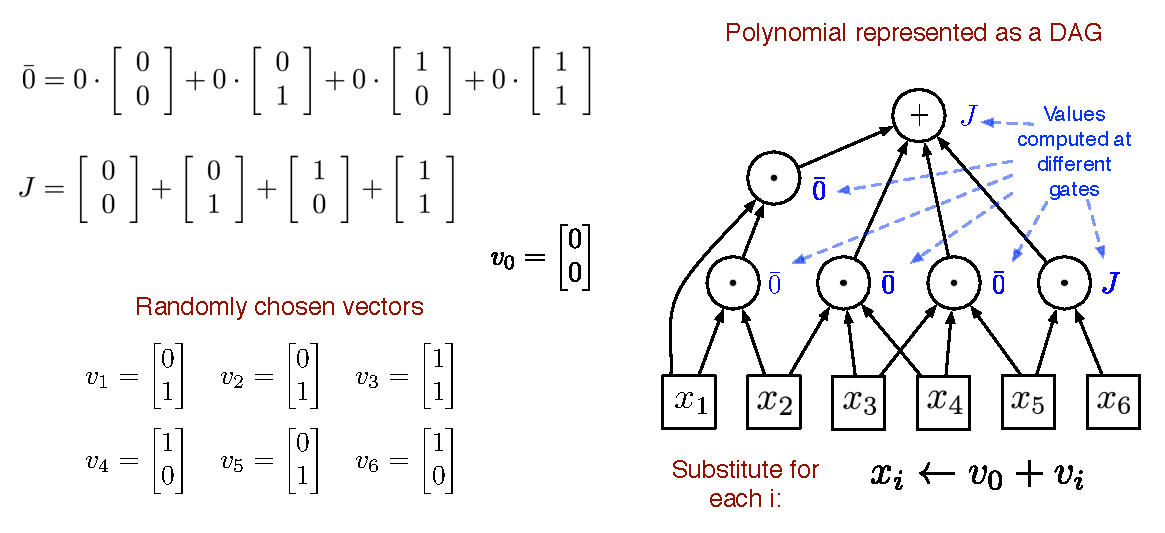
\includegraphics[width=0.5\textwidth]{img/dag3_fixed.pdf}
%\caption{
%\small
%The polynomial $P(x_1,x_2,x_3,x_4, x_5, x_6) = x_1^2x_2 + x_2x_3x_4 + x_3x_4x_5 + x_5x_6$
%represented as a circuit with multiplication ($\cdot$) and addition ($+$) gates, which is a DAG. 
%Each variable $x_i$ is assigned the element $v_0+v_i\in\mathbb{Z}_2[\mathbb{Z}_2^2]$,
%for randomly chosen $v_i\in \mathbb{Z}_2^2$. The computations at each gate
%are in the group algebra, and are shown in blue. The circuit evaluates to the element $J$.
%\vspace{-0.2in}
%}
%\label{fig:dag}
%\end{figure}

\begin{problem} (\textsc{$k$-MLD} problem)
Given a polynomial $P(\cdot)$ defined recursively,
%represented by a DAG $G=(V, E)$, 
in which each monomial
has degree at most $k$ and weight weight $w_S$, determine:
(1) if $P(\cdot)$ has a multilinear term of degree $k$, and 
(2) the maximum weight of any multilinear term, if one exists.
\end{problem}

\subsection{Group Algebras}
\label{sec:grpalgebra}
We discuss some notation from group algebras that is crucial for the paper. 
Let $\mathbb{Z}_2^k$ be the group formed by all the $k$-dimensional binary vectors, and define the group multiplication operation as entry-wise XOR. For example, $\mathbb{Z}_2^2$ consists of the vectors $v_0 = (0, 0), v_1 = (0, 1), v_2 = (1, 0), v_3 = (1, 1)$. We note that $v_0$ is the multiplicative identity of the group, and each element is its own multiplicative inverse: $v_i \cdot v_i = v_0$. Now, we define a group algebra $\mathbb{Z}_2[\mathbb{Z}_2^k]$. Each element in the group algebra is a sum of elements from $\mathbb{Z}_2^k$ with coefficients from $\mathbb{Z}_2$ (i.e., either 1 or 0):
$
\sum_{v\in \mathbb{Z}_2^k} a_v v,
$
where $a_v \in \{0,1\}$. The addition operator of the group algebra is
{\scriptsize
$$
\sum_{v\in \mathbb{Z}_2^k} a_v v + \sum_{v\in \mathbb{Z}_2^k} b_v v = \sum_{v\in \mathbb{Z}_2^k} (a_v + b_v) v,
$$}
where the addition of the coefficients is modulo 2, and the multiplication is defined as
{\scriptsize
$$
\left(\sum_{v\in \mathbb{Z}_2^k} a_v v\right)\left(\sum_{u\in \mathbb{Z}_2^k} b_u u\right) = \sum_{v\in \mathbb{Z}_2^k} (a_v \cdot b_u) (v\cdot u).
$$}


\begin{mdframed}
\scriptsize{
\noindent
\textbf{Example.} For $k=2$, the group algebra $\mathbb{Z}_2[\mathbb{Z}_2^k]$ has
$2^{2^2}=16$ elements, such as
\[
x_1=
0\cdot
\begin{bmatrix}
0\\
0
\end{bmatrix}
+ 1\cdot
\begin{bmatrix}
0\\
1
\end{bmatrix}
+
1\cdot
\begin{bmatrix}
1\\
0
\end{bmatrix}
+ 0\cdot
\begin{bmatrix}
1\\
1
\end{bmatrix}
, \mbox{ which we also write as }
\begin{bmatrix}
0\\
1
\end{bmatrix}
+
\begin{bmatrix}
1\\
0
\end{bmatrix}
\]


\[
x_2 =
\begin{bmatrix}
0\\
0
\end{bmatrix}
+
\begin{bmatrix}
1\\
0
\end{bmatrix}
\]

We have 
\[
x_1 + x_2 = 
\begin{bmatrix}
0\\
0
\end{bmatrix}
+
\begin{bmatrix}
0\\
1
\end{bmatrix}
+ 2
\begin{bmatrix}
1\\
0
\end{bmatrix}
=
\begin{bmatrix}
0\\
0
\end{bmatrix}
+
\begin{bmatrix}
0\\
1
\end{bmatrix}
\]

\[
x_1x_2 = 
\left(
\begin{bmatrix}
0\\
1
\end{bmatrix}
+ 
\begin{bmatrix}
1\\
0
\end{bmatrix}
\right)\cdot 
\left(
\begin{bmatrix}
0\\
0
\end{bmatrix}
+
\begin{bmatrix}
1\\
0
\end{bmatrix}
\right) =
\begin{bmatrix}
0\\
0
\end{bmatrix}
+
\begin{bmatrix}
0\\
1
\end{bmatrix}
+
\begin{bmatrix}
1\\
0
\end{bmatrix}
+
\begin{bmatrix}
1\\
1
\end{bmatrix}
\]
It is easy to check that
\[
x_1^2x_2 = 
0\cdot
\begin{bmatrix}
0\\
0
\end{bmatrix}
+ 0\cdot
\begin{bmatrix}
0\\
1
\end{bmatrix}
+ 0\cdot
\begin{bmatrix}
1\\
0
\end{bmatrix}
+ 0\cdot
\begin{bmatrix}
1\\
1
\end{bmatrix}
= \mathbf{\bar{0}} \text{ (additive identify)}
\]
}
\end{mdframed}

\subsection{Sequential algorithm for Multilinear Detection} 
\label{sec:seq}
We briefly discuss the algorithm of Koutis \cite{koutis:icalp08}, which forms the basis of our paper. An important property is that for any $v_i \in \mathbb{Z}_2^k$, the square of the term $(v_0 + v_i) \in \mathbb{Z}_2[\mathbb{Z}_2^k]$ evaluates to 0:
{\small
$$
(v_0 + v_i)^2 = v_0^2 + 2(v_0\cdot v_i) + v_i^2 = v_0 + (0\mod 2)v_i + v_0 = 2v_0 = 0.
$$}

The main idea in the algorithm of \cite{koutis:icalp08} is that, if we evaluate a polynomial 
over the ``right" algebra, monomials that have square terms evaluate to 0, and the remaining terms,
which are multilinear, do not cancel out, with some probability.
Then, a polynomial $P(X)$ has a $k$ multilinear term if $P(X) \neq 0$. 

We can show that, if we choose a $v_i \in \mathbb{Z}_2^k$ uniformly at random and set $x_i = v_0 + v_i$, then a multilinear monomial does \textbf{not} evaluate to $\bar 0$ with high probability, whereas a monomial with squares is always $\bar 0$ (as in the box above).
The algorithm was later refined in \cite{williams2009finding} by evaluating the polynomial over the group algebra $GF(2^{3 + \log_2k})[\mathbb{Z}_2^k]$, where $GF(p)$ is the finite field of order $p$ \cite{mullen2007finite}. A polynomial $P(x_1,\ldots,x_n)$ with variables from $GF(2^{3 + \log_2k})[\mathbb{Z}_2^k]$ can be evaluated in time $O(2^k poly(n))$ and space $O(kpoly(n))$, resulting in Theorem \ref{theorem:kmld}.

\begin{theorem}[Koutis \cite{koutis:icalp08} and Williams \cite{williams2009finding}]
\label{theorem:kmld}
There exists an algorithm that, given an instance $P(x_1,\ldots,x_n)$ of the \textsc{$k$-MLD} problem, correctly returns ``no" if $P(X)$ does not contain a $k$ multilinear term. Otherwise, if $P(X)$ has a $k$ multilinear term, it returns ``yes" with probability at least 1/5. 
The algorithm has time complexity $O(2^k poly(n))$ and space complexity $O(2^k poly(n))$.
\end{theorem}

At a high level, the algorithm of \cite{koutis:icalp08} involves the following steps.
\begin{enumerate}
\item For each variable $x_i$, sample a vector $v_i$ uniformly at random from $\mathbb{Z}_2^k$ and assign $x_i = (v_0 + v_i) \in \mathbb{Z}_2[\mathbb{Z}_2^k]$.
\item Evaluate the polynomial $P(x_1,\ldots,x_n)$ on this random assignment.
\item If $P(x_1,\ldots,x_n) \neq \bar{0}$ return ``yes"; otherwise, return ``no",
where $\bar{0}$ is the additive identity of the group algebra.
\end{enumerate}

%For the case when a multilinear monomial appears an odd number of times in $P(X)$, Koutis proposed a randomized algorithm that runs in $O(2^k poly(n))$ time and returns an affirmative answer with probability at least $1/4$ \cite{koutis:icalp08}. This algorithm was later extended by Williams \cite{williams2009finding} to allow even repetitions.

%It has been shown that many parameterized graph problems reduce to \textsc{$k$-MLD} \cite{koutis:icalp08,williams2009finding,guillemot2013finding,koutis2012constrained} by efficiently encoding subgraphs of interests as monomials. For example, in the $k$-path problem\footnote{In the $k$-path problem, we are given an unweighted graph $G(V,E)$, and the goal is to decide whether or not there is a simple path containing exactly $k$ nodes in $G$.}, it is possible to recursively construct a polynomial in which each term represents a walk of length $k$, and only multilinear terms correspond to simple paths. Our algorithms in Section \ref{sec:proposed} are based on this methodology: we encode subgraphs of a given size and weight as polynomials, and only connected subgraphs of size at most $k$ where all the nodes are different are multilinear terms.



%Now, we define a group algebra $\mathbb{Z}_2[\mathbb{Z}_2^k]$. Each element in the group algebra is a sum of elements from $\mathbb{Z}_2^k$ with coefficients from $\mathbb{Z}_2$ (i.e., either 1 or 0):
%$$
%\sum_{v\in \mathbb{Z}_2^k} a_v v,
%$$
%where $a_v \in \{0,1\}$. Such element may also be interpreted as a subset of $\mathbb{Z}_2^k$---because of the binary coefficients. The addition operator of the group algebra is
%$$
%\sum_{v\in \mathbb{Z}_2^k} a_v v + \sum_{v\in \mathbb{Z}_2^k} b_v v = \sum_{v\in \mathbb{Z}_2^k} (a_v + b_v) v,
%$$
%where the addition of the coefficients is modulo 2. The multiplication is defined as
%$$
%\left(\sum_{v\in \mathbb{Z}_2^k} a_v v\right)\left(\sum_{u\in \mathbb{Z}_2^k} b_u u\right) = \sum_{v\in \mathbb{Z}_2^k} (a_v \cdot b_u) (v\cdot u).
%$$
%

%The key insight in \cite{koutis:icalp08} is that, for any $v_i \in \mathbb{Z}_2^k$,
%{\small
%$$
%(v_0 + v_i)^2 = v_0^2 + 2(v_0\cdot v_i) + v_i^2 = v_0 + (0\mod 2)v_i + v_0 = 2v_0 = 0 \mod 2.
%$$}
%If we are given a polynomial $P(X)$, and we assign uniformly at random an element $(v_0 + v_i)$ from $\mathbb{Z}_2[\mathbb{Z}_2^k]$ to each $x_i$ variable, then, any monomial with a square term will evaluate to 0. This is called the \emph{annihilation} property. The second key idea is that, under this random assignment, a multilinear monomial does not evaluate to 0 with high probability. This is called the \emph{survival} property. Finally, Koutis shows that a polynomial $P(x_1,\ldots,x_n)$, where the variables are elements from $\mathbb{Z}_2[\mathbb{Z}_2^k]$, can be evaluated in time $O(2^k poly(n))$ and space $O(kpoly(n))$.

%Because of the choice of binary coefficients in the group algebra and the modulo 2 addition operation, any monomial that appears an even number of times in $P(X)$ will evaluate to $0$. In \cite{williams2009finding}, Williams proposes working with the group algebra $GF(2^{3 + \log_2k})[\mathbb{Z}_2^k]$, where $GF(p)$ is the finite field of order $p$ \cite{mullen2007finite}. By using this group algebra, it is unlikely that multilinear monomials evaluate to 0 merely due to repetition, and, at the same time, the annihilation property of \cite{koutis:icalp08} is preserved. We have the following theorem.

%\comment{add sequential algorithm in supplementary and refer to it here}

\subsection{Implementation Using a Matrix Representation $\mathbb{Z}_2[\mathbb{Z}_2^k]$}
Theorem \ref{theorem:kmld} performs operations in the group algebra $\mathbb{Z}_2[\mathbb{Z}_2^k]$,
which takes $O(2^k poly(n))$ space. Koutis \cite{koutis:icalp08} showed that, in fact, the space
complexity can be reduced to $O(k poly(n))$ by using the idea of matrix representations.
%We describe this approach here and then the sequential algorithm \maxwt{} for $k$-MLD. We will develop the parallel version of this algorithm in Section \ref{sec:proposed}.
We use the notation from \cite{koutis:icalp08} and describe it here for completeness.
Let $\rho:\mathbb{Z}_2^k\rightarrow M^{2^k\times 2^k}$ be a matrix representation of
$\mathbb{Z}_2^k$ satisfying $\rho(uv)=\rho(u)\rho(v)$ for all $u, v\in \mathbb{Z}_2^k$.
For $k=1$, the map $\rho:\mathbb{Z}_2\rightarrow M^{2\times 2}$ is defined as
\[
\rho(0) = 
\begin{bmatrix}
1 & 0\\
0 & 1
\end{bmatrix}
\mbox{ and }
\rho(1) = 
\begin{bmatrix}
0 & 1\\
1 & 0
\end{bmatrix}
\]

In general, $\rho(\mathbb{Z}_2^k)$ can be defined recursively. We will use a
simultaneous diagonalization, which allows $\rho(v)$ to be represented as
$\rho(v) = U^{-1}\Lambda_v U$, for each $v\in \mathbb{Z}_2^k$, where $\Lambda_v$ is
a diagonal matrix with its $t$th element equal to $(-1)^{v^T t_{bin}}$,
where $t_{\text{bin}}$ is the $k$-bit binary representation of $t$.
Since the algorithm substitutes $v_0+v_i$ for each variable $x_i$, the $t$th element of the diagonal element in the corresponding
representation for $\rho(v_0+v)$ is $1+(-1)^{v^T t_{bin}}$.

We now describe the sequential algorithm \maxwt{} for the $k$-MLD problem (Algorithm \ref{alg:maxwt}). We are given a graph $G(V,E)$ and a parameter $k$, and the algorithm decides whether or not a polynomial $P$ evaluates to $\bar 0$ in the group algebra. With the matrix representation, the polynomial is evaluated over $2^k$ iterations (lines 6---12). In each iteration, we first initialize $P(i, 1)$, which represents the value of a monomial of degree 1 corresponding to variable $x_i$ (lines 7--8). From there, we compute recursively $P(i,j)$, a polynomial where each term contains $x_i$ and has degree $j$ (lines 9--11). The computation of$P(i,j)$ for a node $i$ uses data from the immediate neighbors of $i$ and all the polynomials of degree $j-1$, which have already been computed at this point. The applications that we consider in Section \ref{sec:applications} have this structure.

\begin{algorithm}{}
\small
\caption{\small \maxwt{}$(G(V, E), k)$.}
\label{alg:maxwt}
\begin{algorithmic}[1]
\STATE \textbf{Input}: Graph $G(V, E)$ and parameter $k$
\STATE\textbf{Output}: ``Yes" if $P$ is non-zero, ``No" otherwise.
\STATE
\STATE For each node $i$, pick a random vector $x_i \in \mathbb{Z}_{2}^k$
\STATE $P = \bar 0$
\STATE \textbf{for} $t = 0$ to $2^{k-1}$
\STATE \quad \textbf{for} $i \in V$ \textbf{do} (base case)
\STATE \quad \quad $P(i, 1) = 1 + (-1)^{x_i^T \cdot t_{\text{bin}}}$
\STATE \quad \textbf{for} $i \in V$, $j = 2$ to $k$ \textbf{do} (recursive step)
\STATE \quad \quad
$P(i,j) = \sum_{u \in \nbr(i)} P(i, [1, j-1])P(u, [1, j-1])$
\STATE \quad $P(j) = \sum_i P(i,j)$ for $i \in V$
\STATE \quad $P = P + P(j)  \mod 2^{k+1}$
\STATE \textbf{return} ``Yes" if $P \neq \bar 0$, else ``No"
\end{algorithmic}
\end{algorithm}
%\section{Sequential algorithm for Multilinear Detection} 
\label{sec:seq}
We briefly discuss the algorithm of Koutis \cite{koutis:icalp08}, which forms the basis of our paper. An important property is that for any $v_i \in \mathbb{Z}_2^k$, the square of the term $(v_0 + v_i) \in \mathbb{Z}_2[\mathbb{Z}_2^k]$ evaluates to 0:
{\small
$$
(v_0 + v_i)^2 = v_0^2 + 2(v_0\cdot v_i) + v_i^2 = v_0 + (0\mod 2)v_i + v_0 = 2v_0 = 0.
$$}

The main idea in the algorithm of \cite{koutis:icalp08} is that, if we evaluate a polynomial 
over the ``right" algebra, monomials that have square terms evaluate to 0, and the remaining terms,
which are multilinear, do not cancel out, with some probability.
Then, a polynomial $P(X)$ has a $k$ multilinear term if $P(X) \neq 0$. 

We can show that, if we choose a $v_i \in \mathbb{Z}_2^k$ uniformly at random and set $x_i = v_0 + v_i$, then a multilinear monomial does \textbf{not} evaluate to $\bar 0$ with high probability, whereas a monomial with squares is always $\bar 0$ (as in the box above).
The algorithm was later refined in \cite{williams2009finding} by evaluating the polynomial over the group algebra $GF(2^{3 + \log_2k})[\mathbb{Z}_2^k]$, where $GF(p)$ is the finite field of order $p$ \cite{mullen2007finite}. A polynomial $P(x_1,\ldots,x_n)$ with variables from $GF(2^{3 + \log_2k})[\mathbb{Z}_2^k]$ can be evaluated in time $O(2^k poly(n))$ and space $O(kpoly(n))$, resulting in Theorem \ref{theorem:kmld}.

\begin{theorem}[Koutis \cite{koutis:icalp08} and Williams \cite{williams2009finding}]
\label{theorem:kmld}
There exists an algorithm that, given an instance $P(x_1,\ldots,x_n)$ of the \textsc{$k$-MLD} problem, correctly returns ``no" if $P(X)$ does not contain a $k$ multilinear term. Otherwise, if $P(X)$ has a $k$ multilinear term, it returns ``yes" with probability at least 1/5. 
The algorithm has time complexity $O(2^k poly(n))$ and space complexity $O(2^k poly(n))$.
\end{theorem}

At a high level, the algorithm of \cite{koutis:icalp08} involves the following steps.
\begin{enumerate}
\item For each variable $x_i$, sample a vector $v_i$ uniformly at random from $\mathbb{Z}_2^k$ and assign $x_i = (v_0 + v_i) \in \mathbb{Z}_2[\mathbb{Z}_2^k]$.
\item Evaluate the polynomial $P(x_1,\ldots,x_n)$ on this random assignment.
\item If $P(x_1,\ldots,x_n) \neq \bar{0}$ return ``yes"; otherwise, return ``no",
where $\bar{0}$ is the additive identity of the group algebra.
\end{enumerate}

%For the case when a multilinear monomial appears an odd number of times in $P(X)$, Koutis proposed a randomized algorithm that runs in $O(2^k poly(n))$ time and returns an affirmative answer with probability at least $1/4$ \cite{koutis:icalp08}. This algorithm was later extended by Williams \cite{williams2009finding} to allow even repetitions.

%It has been shown that many parameterized graph problems reduce to \textsc{$k$-MLD} \cite{koutis:icalp08,williams2009finding,guillemot2013finding,koutis2012constrained} by efficiently encoding subgraphs of interests as monomials. For example, in the $k$-path problem\footnote{In the $k$-path problem, we are given an unweighted graph $G(V,E)$, and the goal is to decide whether or not there is a simple path containing exactly $k$ nodes in $G$.}, it is possible to recursively construct a polynomial in which each term represents a walk of length $k$, and only multilinear terms correspond to simple paths. Our algorithms in Section \ref{sec:proposed} are based on this methodology: we encode subgraphs of a given size and weight as polynomials, and only connected subgraphs of size at most $k$ where all the nodes are different are multilinear terms.



%Now, we define a group algebra $\mathbb{Z}_2[\mathbb{Z}_2^k]$. Each element in the group algebra is a sum of elements from $\mathbb{Z}_2^k$ with coefficients from $\mathbb{Z}_2$ (i.e., either 1 or 0):
%$$
%\sum_{v\in \mathbb{Z}_2^k} a_v v,
%$$
%where $a_v \in \{0,1\}$. Such element may also be interpreted as a subset of $\mathbb{Z}_2^k$---because of the binary coefficients. The addition operator of the group algebra is
%$$
%\sum_{v\in \mathbb{Z}_2^k} a_v v + \sum_{v\in \mathbb{Z}_2^k} b_v v = \sum_{v\in \mathbb{Z}_2^k} (a_v + b_v) v,
%$$
%where the addition of the coefficients is modulo 2. The multiplication is defined as
%$$
%\left(\sum_{v\in \mathbb{Z}_2^k} a_v v\right)\left(\sum_{u\in \mathbb{Z}_2^k} b_u u\right) = \sum_{v\in \mathbb{Z}_2^k} (a_v \cdot b_u) (v\cdot u).
%$$
%

%The key insight in \cite{koutis:icalp08} is that, for any $v_i \in \mathbb{Z}_2^k$,
%{\small
%$$
%(v_0 + v_i)^2 = v_0^2 + 2(v_0\cdot v_i) + v_i^2 = v_0 + (0\mod 2)v_i + v_0 = 2v_0 = 0 \mod 2.
%$$}
%If we are given a polynomial $P(X)$, and we assign uniformly at random an element $(v_0 + v_i)$ from $\mathbb{Z}_2[\mathbb{Z}_2^k]$ to each $x_i$ variable, then, any monomial with a square term will evaluate to 0. This is called the \emph{annihilation} property. The second key idea is that, under this random assignment, a multilinear monomial does not evaluate to 0 with high probability. This is called the \emph{survival} property. Finally, Koutis shows that a polynomial $P(x_1,\ldots,x_n)$, where the variables are elements from $\mathbb{Z}_2[\mathbb{Z}_2^k]$, can be evaluated in time $O(2^k poly(n))$ and space $O(kpoly(n))$.

%Because of the choice of binary coefficients in the group algebra and the modulo 2 addition operation, any monomial that appears an even number of times in $P(X)$ will evaluate to $0$. In \cite{williams2009finding}, Williams proposes working with the group algebra $GF(2^{3 + \log_2k})[\mathbb{Z}_2^k]$, where $GF(p)$ is the finite field of order $p$ \cite{mullen2007finite}. By using this group algebra, it is unlikely that multilinear monomials evaluate to 0 merely due to repetition, and, at the same time, the annihilation property of \cite{koutis:icalp08} is preserved. We have the following theorem.


\subsection{Implementing The Sequential Algorithm Using a Matrix Representation
of $\mathbb{Z}_2[\mathbb{Z}_2^k]$}

Theorem \ref{theorem:kmld} performs operations in the group algebra $\mathbb{Z}_2[\mathbb{Z}_2^k]$,
which takes $O(2^k poly(n))$ space. Koutis \cite{koutis:icalp08} showed that, in fact, the space
complexity can be reduced to $O(k poly(n))$ by using the idea of matrix representations.
%We describe this approach here and then the sequential algorithm \maxwt{} for $k$-MLD. We will develop the parallel version of this algorithm in Section \ref{sec:proposed}.
We use the notation from \cite{koutis:icalp08} and describe it here for completeness.
Let $\rho:\mathbb{Z}_2^k\rightarrow M^{2^k\times 2^k}$ be a matrix representation of
$\mathbb{Z}_2^k$ satisfying $\rho(uv)=\rho(u)\rho(v)$ for all $u, v\in \mathbb{Z}_2^k$.
For $k=1$, the map $\rho:\mathbb{Z}_2\rightarrow M^{2\times 2}$ is defined as
\[
\rho(0) = 
\begin{bmatrix}
1 & 0\\
0 & 1
\end{bmatrix}
\mbox{ and }
\rho(1) = 
\begin{bmatrix}
0 & 1\\
1 & 0
\end{bmatrix}
\]

In general, $\rho(\mathbb{Z}_2^k)$ can be defined recursively. We will use a
simultaneous diagonalization, which allows $\rho(v)$ to be represented as
$\rho(v) = U^{-1}\Lambda_v U$, for each $v\in \mathbb{Z}_2^k$, where $\Lambda_v$ is
a diagonal matrix with its $t$th element equal to $(-1)^{v^T t_{bin}}$,
where $t_{\text{bin}}$ is the $k$-bit binary representation of $t$.
Since the algorithm substitutes $v_0+v_i$ for each variable $x_i$ (as shown in
Figure \ref{fig:dag}), the $t$th element of the diagonal element in the corresponding
representation for $\rho(v_0+v)$ is $1+(-1)^{v^T t_{bin}}$.

%We now describe the sequential algorithm \maxwt{} for the $k$-MLD problem. We are given a graph $G(V,E)$ and a parameter $k$, which together constitute an instance of $k$-MLD. 

%\noindent
%\textbf{High level idea of \textsc{MultilinearDetect-KPath} (Algorithm \ref{alg:multilinear-detect}).}
\subsection{Sequential Algorithm for Scan Statistics (Problem \ref{prob:macs})}
\label{sec:scan-sequential}

For concreteness, we now show how to implement a sequential algorithm for Problem \ref{prob:macs} based on the Multilinear Detection technique. We start by describing how to recursively construct and evaluate a circuit for this problem.

We define the sets $K=\{1,2 \ldots, k\}$ where $k$ is a \emph{size parameter}, and $R=\{0,1,2, \ldots, W(V)\}$, where $W(V) = \sum_v{w(v)}$ is the total weight of the nodes in $G$. For each node $v$, we define a variable $x_v$, and we construct a polynomial over the set of variables $\{x_v: v \in V\}$. Every term---i.e., monomial---in this polynomial will represent a connected subgraph of size at most $k$ and weight at most $W(V)$.
For $i \in K$ and $j \in R$, let $P_v(i,j)$ be the polynomial corresponding to a subgraph (1) containing node $v$, (2) of size $i$, and (3) total weight in
$j$ represents subgraphs of weight 0.
The following recurrence relations describe how the polynomials $P_v(i, j)$ are computed:
\begin{itemize}
\item
$P_v(i, j) = \bar{0}$ for $i \in K$, $j \in R$
\item
$P_v(1, j) = x_v$ for all $v \in V$, $j = w(v)$
\item
for $v \in V$, $i = 2$ to $k$, $j = 0$ to $r$:
\begin{itemize}
\item
$P_v(i,j) = \sum_{u \in \nbr(v)} \sum_{i' = 1}^{i-1}\sum_{j'=0}^j (P_v(i', j') \cdot P_u(i-i', j - j'))$
\end{itemize}
\item
$P(i,j) = \sum_v P_v(i,j)$ for $i \in K$, $j \in R$
\end{itemize}
The above computation can be represented as a polynomial described by a DAG, in which the
nodes corresponding to $P_v(i, j)$ are the intermediate nodes, which are computed by ``$\cdot$'' and ``$+$''
operations.

\noindent
\subsubsection{High level idea of \textsc{MLD-ScanStat} (Algorithm \ref{alg:mld-scanstat})}
After selecting random vectors from $\mathbb{Z}_2^k$ for each circuit input (line 6), 
we compute the polynomial by performing $2^k$ evaluations of the circuit (lines 8--24). 
The $t$-{th} evaluation gives us the value of the $(t + 1)$-th row in the matrix 
representation, as discussed in Section \ref{sec:prelim}. We evaluate the circuit following its recursive definition. First, we initialize the circuit inputs in the base case (lines 11--13) 
to be the $t$-th eigenvalue of their respective matrix representation, which is computed 
as $1 + (-1)^{x_v^T\cdot t_{\text{bin}}}$, where $x_v$ is the random vector assigned to node 
$i$ and $t_{\text{bin}}$ is the $k$-bit binary representation of $t$. 
Then, for each $i \leq k$, we evaluate the circuit by aggregating values from nodes of the form $P_v(i')$, for some $i' < i$, which have already been computed in 
a previous iteration of the \textbf{for} loop. 
%We show an example of this algorithm in Figure \ref{fig:algorithm-example}.

\begin{figure*}[!htbp]
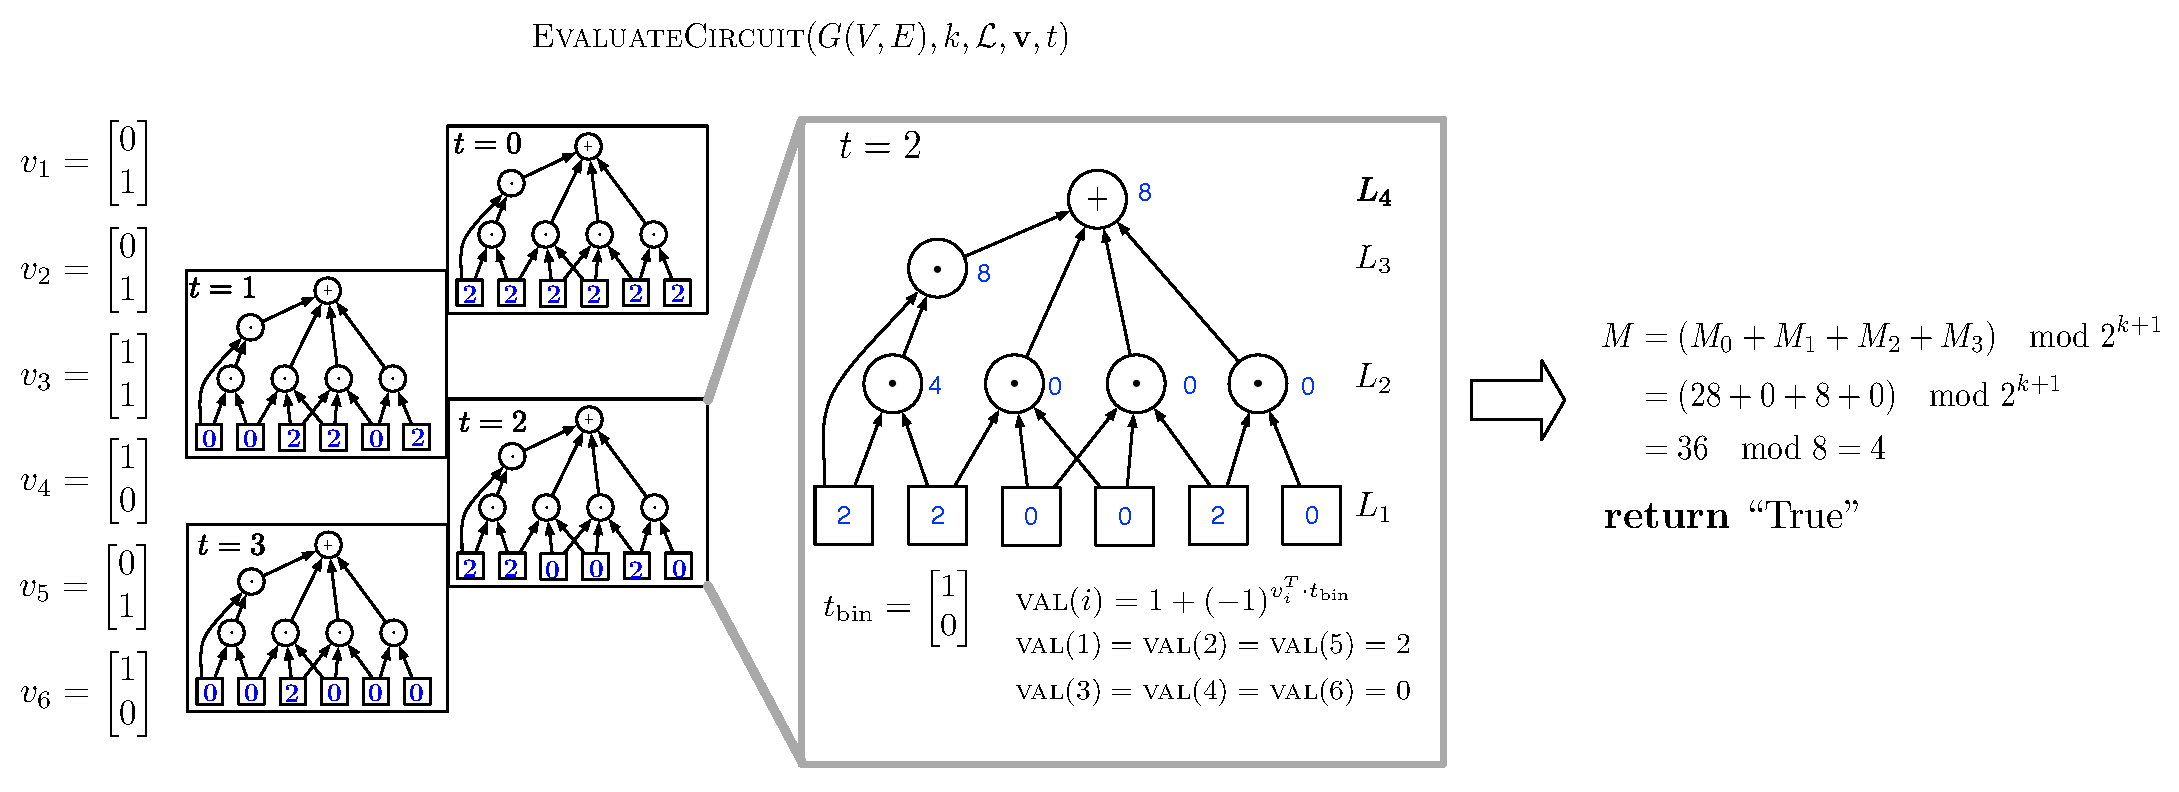
\includegraphics[width=\textwidth]{img/algorithm-example-v2_fixed.pdf}
\caption{
\small
Example of the sequential algorithm \maxwt{}. The input is the circuit $G(V,E)$ from
Figure \ref{fig:dag} with 12 nodes on four levels, $L_1$, $L_2$, $L_3$ and $L_4$, as shown.
The algorithm picks the vectors $v_1,\ldots,v_6$ from $\mathbb{Z}_2^2$, as shown in
the left of the figure. Since $k=2$, there are $2^k=4$ iterations, corresponding to
$t=0,\ldots,3$. The values of $\val(v)=1+(-1)^{v^Tt_{bin}}$ for the $t$th iteration
are shown in blue as the input values. The outputs of the circuit are $M_0, \ldots, M_3$,
with values as shown in the right of the figure. For these choices of the $v_i$'s, the
computed value $M\neq 0 (\text{mod } 2^{k+1})$, which implies the existence of a
multilinear term with $k$ variables. This is true because the term $x_5x_6$ in the
polynomial is indeed multilinear.
%---IDs are in red---$k=2$, and 3 levels. Nodes 1 through 6 are the first level---i.e., the circuit inputs. Nodes 7 through 10 are the second level, all with multiplication operation ($op(i) = \cdot$). The last level only contains the root of the circuit, with addition operation. First, the algorithm generates random vectors $v_i$ for the circuit inputs (bottom left). Then, the circuit is evaluated $2^k$ times by calling procedure \algcircuit{} (center). We show the evaluation for iteration $t=2$. First, we compute the inputs to the circuit as $1 + (-1)^{v_i^T\cdot t_{\text{bin}}}$---this will always be either 2 or 0. From there, we can evaluate the circuit by levels. Finally, back in \maxwt{}, we aggregate the value at root$(G)$ over all the iterations (right). In this case, the polynomial evaluates to $0$, so we return ``False".
%\vspace{-0.2in}
}
\label{fig:algorithm-example}
\end{figure*}

%\begin{algorithm}{}
%\small
%\caption{\maxwt{}$(G(V, E), k$.}
%\label{alg:multilinear-detect}
%\begin{algorithmic}[1]
%\STATE \textbf{Input}: Graph $G(V, E)$, parameter $k$
%\STATE\textbf{Output}: ``True" if circuit evaluation is non-zero. ``False" otherwise.
%\STATE \textbf{Initialize circuit inputs}
%\STATE \textbf{for} node $i \in L_1$ \textbf{do}
%\STATE \quad Let $v_i$ be a random vector from $\mathbb{Z}_{2}^k$
%\STATE \textbf{Initialize the polynomial}
%\STATE Let $M = \bar 0$
%\STATE \textbf{Evaluate circuit for each row of matrix representation}
%\STATE \textbf{for} $t = 0$ to $2^{k-1}$ \textbf{do}
%\STATE \quad $M_t = \algcircuit(G(V, E), k, \mathcal{L}, \mathbf{v}, t)$
%\STATE $M = \sum_{t=0}^{2^{k-1}} M_t \mod 2^{k+1}$
%\STATE \textbf{return} $M \neq 0$
%\STATE
%\STATE \textbf{procedure} \algcircuit{$(G(V, E), k, \mathcal{L}, \mathbf{v}, t)$}
%\STATE \textbf{Input}: Circuit $G(V, E)$, parameter $k$, node levels $\mathcal{L}$, random assigment $\mathbf{v}$, and iteration number $t$
%\STATE\textbf{Output}: Value at root node of $G(V,E)$
%\STATE \textbf{Initialize circuit inputs}
%\STATE \textbf{for} node $i \in L_1$ \textbf{do}
%\STATE \quad $ \val(i) = 1 + (-1)^{v_i^T \cdot t_{\text{bin}}}$
%
%\STATE \textbf{Evaluate the circuit by levels}
%\STATE \textbf{for} $s=2$ to $|\mathcal{L}|$ \textbf{do}
%\STATE \quad \textbf{for} $i \in L_s$ \textbf{do}
%\STATE \qquad \textbf{if} $\op(i) = +$ \textbf{then}
%\STATE \qquad \quad $\val(i) = 0$
%\STATE \qquad \quad \textbf{for} $j \in \pred(i)$ \textbf{do}
%\STATE \qquad \qquad $\val(i) = \val(i) + \val(j)$
%\STATE \qquad \textbf{else} 
%\STATE \qquad \quad $\val(i) = 1$
%\STATE \qquad \quad \textbf{for} $j \in \pred(i)$ \textbf{do}
%\STATE \qquad \qquad $\val(i) = \val(i) \cdot \val(j)$
%
%\STATE \textbf{return} $\val($root$(G))$
%\end{algorithmic}
%\end{algorithm}

\begin{algorithm}{}
\small
\caption{\small \textsc{MLD-ScanStat}$(G(V, E), \mathbf{w}, k, \epsilon, r)$.}
\label{alg:mld-scanstat}
\begin{algorithmic}[1]
\STATE \textbf{Input}: Instance $(G(V, E), \mathbf{w})$ and parameters $k, \epsilon, r$
\STATE\textbf{Output}: "True" if $G$ has a subgraph $S$ with size $i \leq k$ and weight $j \leq r$
\STATE Let $K=\{1,\ldots,k\}, R=\{0, \ldots, r\}$
\STATE \textbf{Initialize the polynomial}
\STATE $P(i, j) = \bar{0}$ for $i \in K$, $j \in R$
\STATE For each node $v$, pick a random vector $x_v \in Q[\mathbb{Z}_{2}^k]$
\STATE \textbf{Evaluate the circuit for each row of matrix representation}
\STATE \textbf{for} $t = 0$ to $2^{k-1}$
\STATE \quad $P_v(i, j) = \bar{0}$ for $i \in K$, $j \in R$
\STATE \quad \textbf{Initialize circuit inputs}
\STATE \quad \textbf{for} $v \in V$ \textbf{do}
\STATE \quad \quad $P_v(1, w(v)) = 1 + (-1)^{x_v^T \cdot t_{\text{bin}}}$
\STATE \quad \textbf{Evaluate circuit recursively}
\STATE \quad \textbf{for} $v \in V$, $i = 2$ to $k$, $j = 0$ to $r$ \textbf{do}
\STATE \qquad $P_v(i,j) = \sum_{u \in \nbr(v)} \sum_{i' = 1}^{i-1}\sum_{j'=0}^j (P_v(i', j') \cdot P_u(i-i', j - j'))$ 
\STATE
\STATE \textbf{return} $P \neq \bar 0$
\end{algorithmic}
\end{algorithm}

%\begin{theorem}[Koutis \cite{koutis:icalp08} and Williams \cite{williams2009finding}]
%\label{theorem:kmld2}
%Algorithm \maxwt{} correctly solves the \textsc{$k$-MLD} problem for an 
%instance $P(x_1,\ldots,x_n)$ with probability at least 1/5 in time
%$O(2^k poly(n))$ and space $O(2^k n)$.
%\end{theorem}

%We note that the success probability in Theorem \ref{theorem:kmld2} can be made very high,
%e.g., $1-\frac{1}{n}$, by running the algorithm $O(\log{n})$ times.

% !TEX root = ./multilinear.tex
\section{Proposed parallel algorithm}
\label{sec:proposed}
We propose a distributed implementation of Algorithm \ref{alg:maxwt} for the $k$-MLD problem. The computation in the recursive step has a \emph{local} structure: a vertex only needs data from its immediate neighbors in the graph. Thus, Algorithm \ref{alg:maxwt} is amenable to a vertex-centric parallelization. However, as we describe below, there are various techniques and implementation details needed to make the computation scalable and overcome high communication overheads. \comment{Someone revise the last 2 sentences, please.} 

%Both problems \ref{prob:trees} and \ref{prob:macs} can be reduced to instances of the $k$-MLD problem, as we will discuss later in Section \ref{sec:applications}; this will automatically lead to corresponding parallel algorithms for both these problems.

\subsection{Overview of the Algorithm \parmaxwt{}}
Let $N$ denote the total number of
processors or parallel units available. Quantities $N_1$ and $N_2$ are parameters for controlling the parallelism
in different parts of the algorithm.  
We assume $2^k/N_2$ and $N/N_1$ are integers, in order to avoid cluttering the
notation using ceiling and floor of these quantities, respectively.
%The algorithm involves solving a dynamic program repeatedly for a certain number of rounds. 
The algorithm involves solving a dynamic program $2^k$ times; these $2^k$ loops are independent, and we divide them into \emph{phases} of size $N_2$ each, so that a total of $2^k/N_2$ phases have to be run. These are run in $2^k/(N_2N/N_1)$ ``batches", where each batch involves running $N/N_1$ phases. A phase involves a call to the subroutine \parcircuit{}.
See Figure \ref{fig:parallel} for an illustration of this structure.

We partition the graph $G$ into $N_1$ parts, denoted by
$\mathcal{P}=\{G^1, \ldots, G^{N_1}\}$; desirable properties of the partition will be discussed later. For a partition $j$, let $\textsc{Deg}(j)$ be the \emph{degree} of $j$, defined as the number of edges connecting nodes in $j$ to nodes in some other partition:
$$
\textsc{Deg}(j) = |\{(u, v): (u, v) \in G, u \in G^i, v \not \in G^i\}|,
$$
and let \maxdeg{} $ = \max_{j} \textsc{Deg}(j)$. Also, let $\maxload{} = \max_j |G^j|$ be the maximum ``load" or number of vertices on any partition. We will analyze the performance of our algorithm in terms of $\maxload{}$ and $\maxdeg{}$.

%\begin{figure}[h]
%\centering
%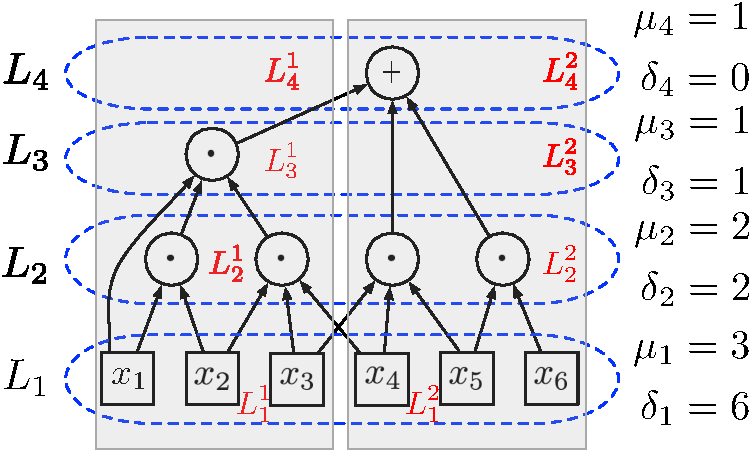
\includegraphics[width=0.4\textwidth]{img/dag4.pdf}
%\caption{
%\small
%Illustration of the level sets and associated quantities for the DAG in
%Figure \ref{fig:dag}, corresponding to a partition into two parts. 
%%\vspace{-0.2in}
%}
%\label{fig:dag4}
%\end{figure}

%\noindent
%\textbf{High level overview.}
We describe the main intuition of the steps of Algorithm \parmaxwt{} below.
\begin{enumerate}
\item
The algorithm starts with the partitioning $\mathcal{P}$ of the graph $G$.
%We discuss its complexity and implementation in Section \ref{sec:partition}.
\item
The algorithm runs $\log{1/\epsilon}\log{5/4}$ rounds, each of which involves $2^k$ iterations.
Here, $\epsilon\in(0, 1)$ is a parameter, which governs the success probability\footnote{As per Theorem \ref{theorem:kmld}, Algorithm \maxwt{} succeeds with probability 1/5, so we need to run it multiple times}. Each such round with $2^k$ iterations is partitioned into
$2^k/N_2$ phases in the while loop in lines 8--12 of \parmaxwt{}, which are completely independent of other phases.
\item
In the $t$th phase, Algorithm \parcircuit{} uses a vector of size $N_2$ to store
$\langle P(i, tN_2),\ldots, P(i, (t+1)N_2-1)\rangle$ for each node $i$; these
will be computed simultaneously using a dynamic program.
\item
In the $t$th phase, for each node $i$, we use the vector for each neighbor $u$ of $i$ to compute $\langle P(i, tN_2),\ldots, P(i, (t+1)N_2-1)\rangle$.
If $u$ is in the same partition, then its data is available on that processor. For every neighbor $u$ in a different partition, $u$ has to send a message with $\langle P(u, tN_2),\ldots, P(u, (t+1)N_2-1)\rangle$, introducing a communication overhead.
\item
We use $\rootsum^{\ell}_t = P(tN_2, k) + \ldots P((t+1)N_2-1, k)$ 
to denote the sum of the values of the root node within the phase, for round $\ell$. These are summed up
over all the phases within round $\ell$ to compute the total, denoted by $P^{\ell}$.
\end{enumerate}

\begin{figure}[h]
\centering
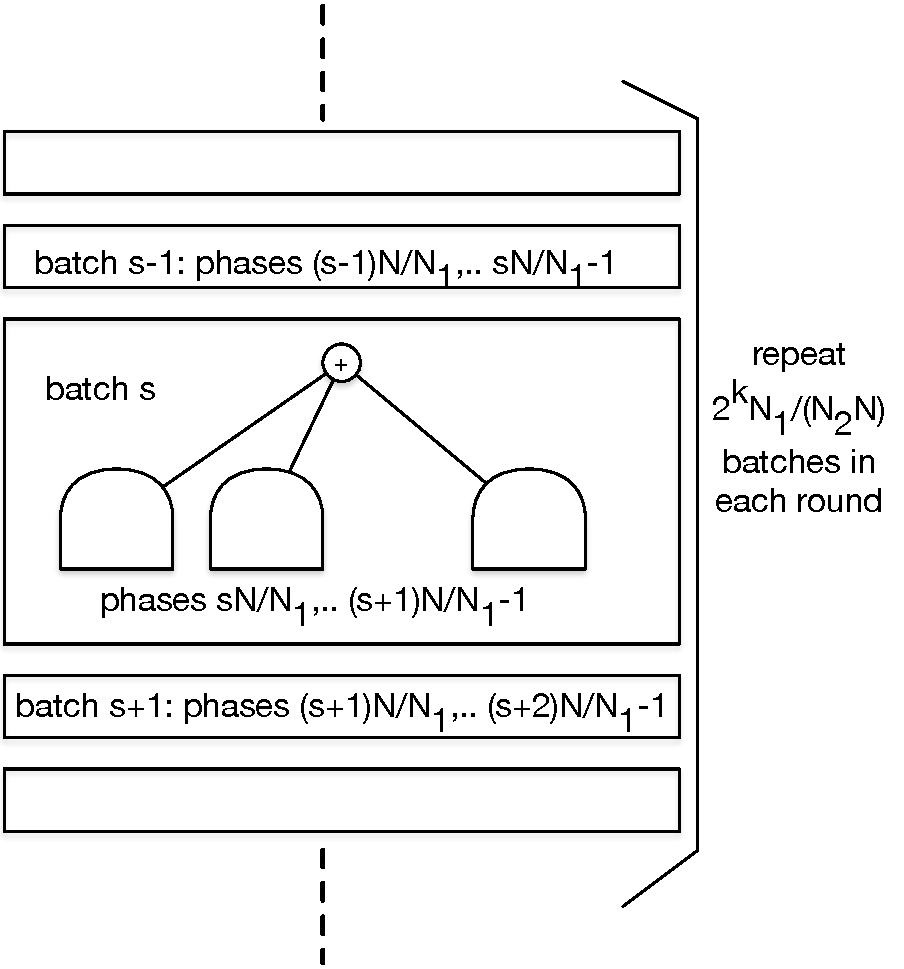
\includegraphics[width=0.3\textwidth]{img/parallel.pdf}
\caption{
\small
Schematic structure of \parmaxwt{}: we run $(\log{1/\epsilon})/(\log{5/4})$ rounds.
Each round is partitioned into $2^kN_1/(N_2N)$ batches, and each batch involves
$N/N_1$ phases being run simultaneously. Each phase involves an evaluation of the
polynomial on $N_2$ iterations in algorithm \parcircuit{}, which are then summed up.
}
\label{fig:parallel}
\end{figure}

\begin{algorithm}{}
\small
\caption{\parmaxwt{}$(G, k, \epsilon, N_1, N_2)$.}
\label{alg:parallel-kMLD} 
\begin{algorithmic}[1]
\STATE \textbf{Input}: Graph $G=(V,E)$, parameter $k$,
confidence parameter $\epsilon\in (0, 1)$, parameters $N_1$ and $N_2$, which guide the parallelism.
\STATE\textbf{Output}: ``Yes" if circuit evaluation is non-zero. ``No" otherwise.

\STATE Let $v_i \in \mathbb{Z}_2^k$ be a random vector for each node $i$
\STATE Let $P = \bar 0$ be the polynomial
\STATE Let $N_1$ denote the number of processors used for each iteration.
%Let $\mathcal{P}=\{G^1= (V^1, E^1), \ldots, G^{N_1}=(V^{N_1}, E^{N_1})\}$ denote the corresponding
Let $\mathcal{P}=\{G^1, \ldots, G^{N_1}\}$ denote the corresponding partition of the graph into $N_1$ parts.
\STATE \textbf{for} $\ell=1$ to $(\log{1/\epsilon})/(\log{5/4})$ 
\STATE \quad $P^{\ell}=0$
\STATE \quad \textbf{while} $s \leq \frac{2^k/N_2}{N/N_1}$ \textbf{do}
\STATE \quad \quad \textbf{for} $t =s N/N_1$ to $(s+ 1)N/N_1$ \textbf{do in parallel}
\STATE \quad \qquad  $\rootsum^{\ell}_{t} = \parcircuit(G, k, \mathbf{v}, t, N_2, N_1, \mathcal{P})$
\STATE \quad \quad \textsc{MpiBarrier}
\STATE \quad \quad $P^{\ell} = P^{\ell} + \sum_{t=s N/N_1}^{(s+1)N/N_1} \rootsum^{\ell}_{t} \mod 2^{k+1}$ using \textsc{MpiReduce}
\STATE \textbf{if} $P^{\ell}\neq 0$ for some $\ell$
\STATE \quad \textbf{return} \textbf{True}
\STATE \textbf{else} 
\STATE \quad \textbf{return} \textbf{False}
\end{algorithmic}
\end{algorithm}

\begin{algorithm}{}
\small
\caption{\parcircuit{$(G, k, \mathbf{v}, t, N_2, N_1, \mathcal{P})$}}
\label{alg:parEvaluate} 
\begin{algorithmic}[1]
%\STATE \textbf{Procedure} \parcircuit{$(G(V, E), k, \mathcal{L}, \mathbf{v}, t, p)$}
\STATE \textbf{Input:} Circuit $G$, parameter $k$, random assignment $\mathbf{v}$, phase number $t$, number of iterations within phase $N_2$, number of partitions $N_1$, and partitioning $\mathcal{P}$
\STATE
\STATE \textbf{for} processor $s$ \textbf{do in parallel}
\STATE \quad \textbf{Base case}
\STATE \quad \textbf{for} node $i \in G^s$ and iteration $q \in tN_2,\ldots,(t+1)N_2-1$ \textbf{do}
\STATE \qquad $ P(i, q, 1) = 1 + (-1)^{v_i^T \cdot q_{\text{bin}}}$

\STATE \quad \textbf{Recursive step}
\STATE \quad \textbf{for} $j=2$ to $k$ \textbf{do}
\STATE \qquad \textbf{for} vertex $i \in G^s$ \textbf{do}
\STATE \qquad \quad \textbf{for} all $q$ set $P(i,q,  j) = \bar 0$
\STATE \qquad \quad \textbf{for} each incoming message $\langle u, P(u, q, [1, j-1])\rangle$ \textbf{do}
\STATE \qquad \qquad $P(i, q, j)=$ $P(i, q, [1, j-1])  P(u, q, [1, j-1])$
\STATE \qquad \quad  \textbf{Send result to neighbors}
\STATE \qquad \quad \textbf{for} $u \in \nbr(i)\setminus G^s$ \textbf{do}
\STATE \qquad \qquad \textbf{Send} $\langle i, P(i, q, j)\rangle$
\STATE \textsc{MpiBarrier}
\STATE \textbf{return} $\sum_q \sum_i P(i, q, k)$
\end{algorithmic}
\end{algorithm}

Recall the definition of $\maxdeg{}$ corresponding to the partitioning $\mathcal{P}$.
Further, let $c_1$ and $c_2$ denote the time for unit computation at any node in $G$
and the unit communication along any edge, respectively, in the Algorithm \parcircuit{}.
The time and communication complexity of algorithm \parmaxwt{} is summarized below
in terms of these parameters. 

\begin{theorem}
\label{thm:parmaxwt}
For any $\epsilon\in(0, 1)$,
Algorithm \parmaxwt{} solves the \textsc{$k$-MLD} problem for an
instance $P(x_1,\ldots,x_n)$ with probability at least $1-\epsilon$. The total time for
computation and communication are $O\left(c_1\frac{2^kN_1}{N}k \maxload{}\log{1/\epsilon}\right)$ 
and $O\left(c_2\frac{2^kN_1}{N N_2}k \maxdeg{}\log{1/\epsilon}\right)$, respectively.
\end{theorem}
\begin{proof} (Sketch)
First, we argue the correctness. 
The call to \parcircuit{} evaluates the polynomial bottom up in parallel for all iterations in the
$t$th phase, namely iterations $tN_2,\ldots,(t+1)N_2-1$. The vector
$\langle P(tN_2, k),  \ldots ,P((t+1)N_2-1, k)\rangle$
is the final evaluation of the polynomial for each iteration in this phase.
Each call to \parcircuit{} in Algorithm \parmaxwt{}
returns the sum of these values for phase $t$.
Each round of Algorithm \parmaxwt{}, corresponding to the value of
$\ell$ in the outer for loop in lines 6--12, goes over all phases, and
calls \parcircuit{}. Therefore, within round $\ell$, $P^{\ell}$ denotes the
sum of the polynomial evaluation over all the $2^k$ iterations within that round.
If $P(\cdot)$ has a multilinear term,
from \cite{koutis:icalp08,williams2009finding}, $P^{\ell}\neq 0 \text{ mod }2^{k+1}$ with
probability at least $1/5$. This implies that 
$\Pr[P^{\ell} = 0,\ \forall \ell] = (\frac{4}{5})^{(\log{1/\epsilon})/(\log{5/4})}\leq\epsilon$,
so that with probability at least $1-\epsilon$, \parmaxwt{} returns true.  On the other hand,
if $P(\cdot)$ has no multilinear term, then with probability $1$, $P^{\ell}=0$ for all $\ell$.
Therefore, \parmaxwt{} correctly solves the \textsc{$k$-MLD} problem with probability
at least $1-\epsilon$.

Next, we consider the computation and communication time complexity. 
The algorithm \parcircuit{} computes the polynomial for each degree up to $k$ within each iteration.
Therefore, the computation time in a phase $t$ is 
$O(c_1 k \max_j |G^j| N_2) = O(c_1k\maxload{}N_2)$, which is the maximum time for any processor. Therefore, the total compute time over all the rounds is
$O(\frac{2^k/N_2}{N/N_1} c_1 k \maxload{} N_2)$, which corresponds to the bound in the theorem.
After any evaluation in the recursive step, the results have to be sent on all neighbors, for every pair of
processors $s, s'$. Therefore, the maximum number of messages in one iteration of the loop in lines 8--15 is $\maxdeg{}$, and the total number of messages, over all the rounds, is
$O(\frac{2^k/N_2}{N/N_1} \maxdeg{}) = O(\frac{2^kN_1}{N N_2} \maxdeg{})$.
\end{proof}

%%\subsection{Partition and Load Balancing}
%%\label{sec:partition}
%%
%%From Theorem \ref{thm:parmaxwt}, the performance of Algorithm \parmaxwt{} depends crucially
%%on the partitioning. Specifically, the partition should be ``vertical'', i.e., one which achieves
%%load balance across each level and also minimizes the edge cut, which is formalized by
%%\[
%%\text{cost}(\mathcal{P}) = \sum_s (c_1\maxload{}_s + c_2\maxdeg{}_s)
%%\]
%%
%%However, finding a partitioning $\mathcal{P}$ that minimizes the above objective
%%$\text{cost}(\mathcal{P})$ is NP-hard, in general, as summarized below. The proof
%%is omitted for brevity.
%%
%%\begin{lemma}
%%\label{lemma:partition}
%%Given a DAG $G=(V, E)$ and per-unit computation and communication costs $c_1$ and $c_2$,
%%respectively, finding a partitioning $\mathcal{P}$ with the minimum cost is NP-hard, in general.
%%\end{lemma}
%%
%%In light of Lemma \ref{lemma:partition}, we consider two heuristics: finding balanced
%%partitions in each level, and combining them, as well as METIS \cite{karypis:sijsc99}.

%We partition the circuit ``vertically"; that is, each processor gets a subset of nodes for each level in $\mathcal{L}$. Let $f(i)$ be the cost of evaluating node $v$. Then, we want to find a partition, such that
%$$
%\sum_{v \in V^p} f(i) \approx \frac{1}{p}\sum_{i \in V} f(i).
%$$

%\subsection{Analysis of Algorithm \parmaxwt{}}
%\subsubsection{Time Complexity}
%The \textbf{while} loop in lines 8--13 of \parmaxwt{} runs for at most $\frac{2^k}{P / p}$ iterations. For each iteration, each partition does work in the order $O(\frac{1}{p}\sum_{i \in V} f(i))$, so the total running time is $O(\frac{1}{p}(2^k f(V)))$.
%\subsubsection{Number of Messages}
%We assume that we have $P$ processors available and that $G$ does not fit in the memory of a single computing node. We have to use $p \leq P$ processors to store the graph in memory. We propose an MPI algorithm with roughly the following steps:

%\begin{enumerate}
%\item \parmaxwt{} Algorithm \ref{alg:parallel-kMLD}
%\item Determine $p$, the number of processors needed to store the graph.
%\item We have to run the loop from line 9 of \maxwt{}. Each of the $2^k$ iteration is independent of the others, so we can run $\lfloor{P/p}\rfloor$ iterations in parallel.
%\item \parcircuit{} Algorithm \ref{alg:parEvaluate}
%\item For each iteration $t$, we first partition the circuit into $p$ parts, and we evaluate these parts in parallel.
%\item For each partition $p'$, we evaluate the circuit by levels, as in \maxwt{}. 
%\item For each node $i$ that we evaluate, we compute $m(i)$ using the $m(j)$ value for each predecessor $j$. if a predecessor $j$ is in the same partition $p'$, then, we can simply read $m(j)$, as in the sequential algorithm. For every predecessor $j$ in a different partition, $j$ has to send a message with $m(j)$, introducing a communication overhead.
%\item We aggregate the value at root$(G)$ over all $2^{k}$ iterations to get the final solution.
%\end{enumerate}

%\noindent
%\textbf{Algorithm \ref{alg:parallel-kMLD}}: \parmaxwt{}\\
%1. Determine $p$, the number of processors needed to store the graph.\\
%2. We have to run the loop from line 9 of \maxwt{}. Each of the $2^k$ iteration is independent of the others, so we can run $\lfloor{P/p}\rfloor$ iterations in parallel.\\
%\textbf{Algorithm \ref{alg:parEvaluate}}: \parcircuit{} \\
%3. For each iteration $t$, we first partition the circuit into $p$ parts, and we evaluate these parts in parallel.\\
%4. For each partition $p'$, we evaluate the circuit by levels, as in \maxwt{}. \\
%5. For each node $i$ that we evaluate, we compute $m(i)$ using the $m(j)$ value for each predecessor $j$. If a predecessor $j$ is in the same partition $p'$, then, we can simply read $m(j)$, as in the sequential algorithm. For every predecessor $j$ in a different partition, $j$ has to send a message with $m(j)$, introducing a communication overhead.\\
%6. We aggregate the value at root$(G)$ over all $2^{k}$ iterations to get the final solution.

\section{$k$-Tree and graph scan statistics}
\label{sec:applications}
We now describe how \ouralgo{} for the $k$-path problem can be extended to 
parallel algorithms for finding trees and optimizing scan statistics. We discuss here how the corresponding polynomials are constructed recursively and evaluated in the subroutines \parcircuittree{} and \parcircuitscan{};
the main Algorithm \ouralgo{} remains unchanged.

\subsection{$k$-Tree}
\label{sec:apps-trees}
\begin{figure}[h]
\vspace{-0.2in}
\centering
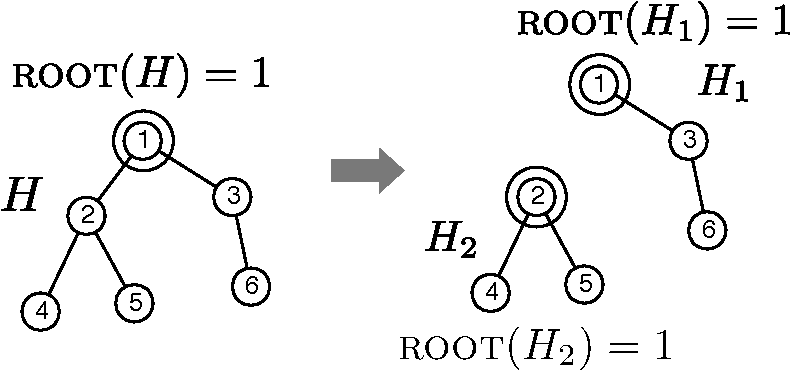
\includegraphics[width=0.37\textwidth]{img/trees.pdf}
\caption{
\small
Tree $H$ with $\myroot(H)=1$ is decomposed into trees $H_1$ and $H_2$ by
removing edge $(1, 2)$: $\myroot(H_1)=1$ and $\myroot(H_2)=2$.
%\vspace{-0.2in}
}
\label{fig:trees}
\end{figure}
We describe how an instance of $k$-Tree with graph $G=(V,E)$ and tree $H=(V^H, E^H)$
is reduced to a $k$-MLD instance. We consider the tree $H$ to be rooted,
and let $\myroot(H)$ be the root node, selected arbitrarily. We consider a hierarchical
structure among subtrees of $H$ in the following manner: consider any node $u\in\nbr(\myroot(H))$.
Let $H_1$ and $H_2$ denote the subtrees or \emph{children} obtained upon deleting the edge $(u, \myroot(H))$,
with $\myroot(H)\in H_1$ and $u\in H_2$. We set $\myroot(H_1)=\myroot(H)$ and $\myroot(H_2)=u$.
This process is illustrated in Figure \ref{fig:trees}.
The subtrees $H_1$ and $H_2$ are further partitioned in a recursive manner until
all trees have a single node.
We define the polynomials $P(i, H')$, which will correspond to all layouts (not necessarily
isomorphisms) of $H'$ with $\myroot(H')=i$ for all nodes $i \in V$, as follows:
\begin{itemize}
\item
If $H'$ consists of a single node, $P(i, H') = x_i$
\item
Else, 
$P(i, H') = \sum_{u\in\nbr(i)} P(i, H'_1)P(u, H'_2)$, where
$H'_1$ and $H'_2$ are the children of $H'$.
\item
Finally, we have
$P(x_1,\ldots, x_n)= \sum_{i \in V} P(i, H)$
\end{itemize}

By using ideas from \cite{alon2008biomolecular}, it can be verified that the tree $H$ is a subgraph of $G$ if and only if the
polynomial $P(x_1,\ldots,x_n)$ has a multilinear term. Algorithm \parcircuittree{}
evaluates this polynomial analogous to Algorithm \ref{alg:parEvaluatepath} from Section \ref{sec:proposed}. The performance of \ouralgo{} using \parcircuittree{} is summarized below.

\begin{lemma}
\label{lemma:parmaxwt-tree}
For any $\epsilon\in(0, 1)$,
Algorithm \ouralgo{}, using \parcircuittree{}, solves the \textsc{$k$-Tree} problem for an
instance $(G, H)$ with probability at least $1-\epsilon$. The total time for
computation and communication are $O\left(c_1\frac{2^kN_1}{N}|\mathcal{T}| \maxload{}\log{1/\epsilon}\right)$ 
and $O\left(c_2\frac{2^kN_1}{N N_2}|\mathcal{T}| \maxdeg{}\log{1/\epsilon}\right)$, respectively.
\end{lemma}

\begin{algorithm}{}
\small
\caption{\parcircuittree{$(G(V, E), H(V^H, E^H), \mathbf{v}, t, N_2, N_1, \mathcal{P})$}}
\label{alg:parEvaluatepath} 
\begin{algorithmic}[1]
\STATE \textbf{Input:} Graph $G(V, E)$, tree $H(V^H, E^H)$ with $k$ vertices, 
random assignment $\mathbf{v}$, phase number $t$, number of iterations within phase $N_2$,
number of partitions $N_1$, and partitioning $\mathcal{P}$
\STATE \textbf{Output:} The value of the polynomial corresponding to $k$-tree in the iterations within a phase
\STATE
\STATE Let $\mathcal{T}$ be a collection of subtrees of $H$ sorted by size
\STATE \textbf{for} each processor $s$\textbf{do in parallel}
\STATE \quad \textbf{for} each subtree $j \in \mathcal{T}$ \textbf{do}
\STATE \quad \quad \textbf{for} node $i\in G^s$ and iteration $q\in [tN_2,(t+1)N_2 - 1]$ \textbf{do}
\STATE \quad \quad \quad \textbf{if} $|j|=1$ \textbf{then}
\STATE \quad \quad \quad \quad $P(i, q, j) = 1 + (-1)^{v_i^T \cdot q_{\text{bin}}}$
\STATE \quad \quad \quad \textbf{else}
\STATE \quad \quad \quad \quad set $P(i,q, j) = 0$
\STATE \quad \quad \quad \quad let $j'$ and $j''$ be the children of subtree $j$
\STATE \quad \quad \quad \quad \quad \textbf{for} each incoming message $\langle u, P(u, q, j'')\rangle$ \textbf{do}
\STATE \quad \quad \quad \quad \quad \quad $P(i, q, j)= P(i, q, j) + P(i, q, j')  P(u, q, j'')$
\STATE \quad \quad \quad \textbf{Send result to neighbors}
\STATE \quad \quad \quad  \textbf{for} $u \in \nbr(i)\setminus G^s$ \textbf{do}
\STATE \quad \quad \quad \quad \textbf{Send} $\langle i, P(i, q, j)\rangle$
\STATE \textsc{MpiBarrier}
\STATE \textbf{return} $\sum_q \sum_i P(i, q, H)$
\end{algorithmic}
\end{algorithm}

More generally, we consider a weighted version of the problem, where the goal is to find an embedding of the maximum weight. We also note that the algorithm can be generalized to find motifs of bounded treewidth, similar to algorithms based on the color coding technique. \cite{alon1995color}.

\iffalse
\comment{move the rest of this to the supplementary}

\begin{figure}[h]
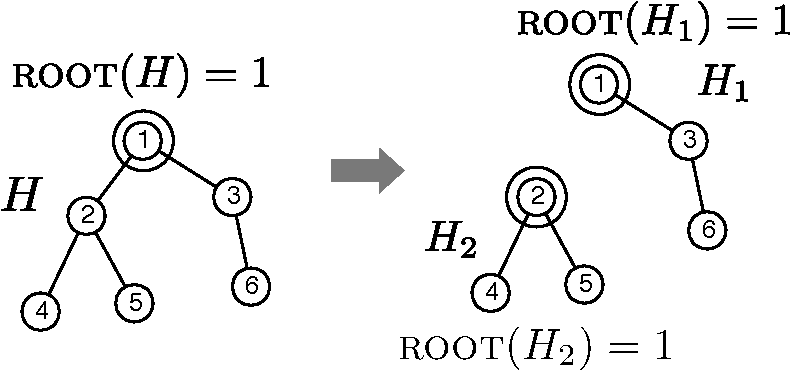
\includegraphics[width=0.4\textwidth]{img/trees.pdf}
\caption{
\small
Tree $H$ with $\myroot(H)=1$. It is decomposed into trees $H_1$ and $H_2$ by
removing the edge $(1, 2)$. $\myroot(H_1)=1$ and $\myroot(H_2)=2$.
%\vspace{-0.2in}
}
\label{fig:trees}
\end{figure}
Next, we consider the case where $H$ is a tree. We consider the tree to be rooted,
and let $\myroot(H)$ be the root node, selected arbitrarily. We consider a hierarchical
structure among subtrees of $H$ in the following manner: consider any node $u\in\nbr(\myroot(H))$.
Let $H_1$ and $H_2$ denote the subtrees obtained upon deleting the edge $(u, \myroot(H))$,
with $\myroot(H)\in H_1$ and $u\in H_2$. We set $\myroot(H_1)=\myroot(H)$ and $\myroot(H_2)=u$.
This process is illustrated i Figure \ref{fig:trees}.
The subtrees $H_1$ and $H_2$ are further partitioned in a recursive manner, till
all trees have a single node. For an intermediate tree $H'$ in this process,
let $\textsc{child}_1(H')$ and $\textsc{child}_2(H')$ denote the two child trees
resulting from the tree $H'$. Let $\textsc{parent}(H')=H''$ be the tree such that
either $\textsc{child}_1(H'')= H'$ or $\textsc{child}_2(H'') = H'$.
We define the polynomials $P_v(H')$, which will correspond to all layouts (not necessarily
isomorphisms) of $H'$ with $\myroot(H')=v$, in the following manner:
\begin{itemize}
\item
If $H'$ consists of a single node, $P_v(H') = x_v$
\item
Else, 
$P_v(H') = \sum_{u\in\nbr(v)} P_v(H'_1)P_u(H'_2)$, where
$H'_1$ and $H'_2$ denote $\textsc{child}_1(H')$ and $\textsc{child}_2(H')$, respectively.
\item
Finally, we have
$P(x_1,\ldots, x_n)= \sum_v P_v(H)$
\end{itemize}

More generally, we consider a weighted version of the problem, where the goal is to find an embedding of the maximum weight. We also note that the algorithm can be generalized to find motifs of bounded treewidth similar to algorithms based on the color coding technique. \cite{alon1995color}.
\fi 

\subsection{Scan Statistics}
\label{sec:apps-scanstat}
%For concreteness, we now show how to implement a sequential algorithm for Problem \ref{prob:macs} based on the Multilinear Detection technique. We start by describing how to recursively construct and evaluate a circuit for this problem.
Let $W(V) = \sum_{i\in V}{w(i)}$ be the total weight of the nodes in $G$. For each node $i$, we define a variable $x_i$, and we construct a polynomial over the set of variables $\{x_i: i \in V\}$. Every term---i.e., monomial---in this polynomial will represent a connected subgraph of size at most $k$ and weight at most $W(V)$.
For $j \leq k$ and $z \leq W(V)$, let $P(i,j,z)$ be the polynomial corresponding to a subgraph (1) containing node $i$, (2) of size $j$, and (3) total weight $z$. The following recurrence relations describe how the polynomials $P(i, j, z)$ are computed:
\begin{itemize}
\item
$P(i, 1, z) = x_i$ for all $i \in V$, $z = w(v)$
\item
For $i \in V$, $j = 2$ to $k$, $z = 0$ to $W(V)$, 
$P(i,j, z) = \sum_{u \in \nbr(i)} \sum_{j' = 1}^{j-1}\sum_{z'=0}^z (P(i, j', z') \cdot P(u, j - j', z-z'))$
\item
$P(j, z) = \sum_i P(i,j, z)$ for $j \leq k$, $z \leq W(V)$
\end{itemize}
Algorithm \ref{alg:parEvaluateScanStat} maintains variables $P(i, q, j, z)$ for every node $i$, $j\leq k$, $z \leq W(V)$, and iteration $q$ within phase $t$. It can be verified \cite{cadena:bigdata17} that the input graph $G$ has a connected subgraph $S$ of size $j$ and weight $z$ if and only if the corresponding polynomial $P(j, z)$ has a multilinear term.
We have the following lemma.
%The performance of \ouralgo{}, using \parcircuittree{} is summarized below.

\begin{lemma}
\label{lemma:parmaxwt-scan}
For any $\epsilon\in(0, 1)$,
Algorithm \ouralgo{}, using \parcircuitscan{}, solves the \textsc{Scan Statistics} problem for an
instance $(G, k, \mathbf{w})$, with probability at least $1-\epsilon$. The total time for
computation and communication are $O\left(c_1\frac{2^kN_1}{N}W(V)^2k^2 \maxload{}\log{1/\epsilon}\right)$ 
and $O\left(c_2\frac{2^kN_1}{N N_2}W(V)^2k^2 \maxdeg{}\log{1/\epsilon}\right)$, respectively.
\end{lemma}

We note that the performance for scan statistics can be improved significantly by rounding the weights, using a standard technique as in the Knapsack problem \cite{cadena:bigdata17}.

%\noindent
%\subsubsection{High level idea of \textsc{MLD-ScanStat} (Algorithm \ref{alg:mld-scanstat})}
%After selecting random vectors from $\mathbb{Z}_2^k$ for each circuit input (line 6), 
%we compute the polynomial by performing $2^k$ evaluations of the circuit (lines 8--24). 
%The $t$-{th} evaluation gives us the value of the $(t + 1)$-th row in the matrix 
%representation, as discussed in Section \ref{sec:prelim}. We evaluate the circuit following its recursive definition. First, we initialize the circuit inputs in the base case (lines 11--13) 
%to be the $t$-th eigenvalue of their respective matrix representation, which is computed 
%as $1 + (-1)^{x_v^T\cdot t_{\text{bin}}}$, where $x_v$ is the random vector assigned to node 
%$i$ and $t_{\text{bin}}$ is the $k$-bit binary representation of $t$. 
%Then, for each $i \leq k$, we evaluate the circuit by aggregating values from nodes of the form $P_v(i')$, for some $i' < i$, which have already been computed in 
%a previous iteration of the \textbf{for} loop. 
%We show an example of this algorithm in Figure \ref{fig:algorithm-example}.

%%%\begin{figure*}[!htbp]
%%%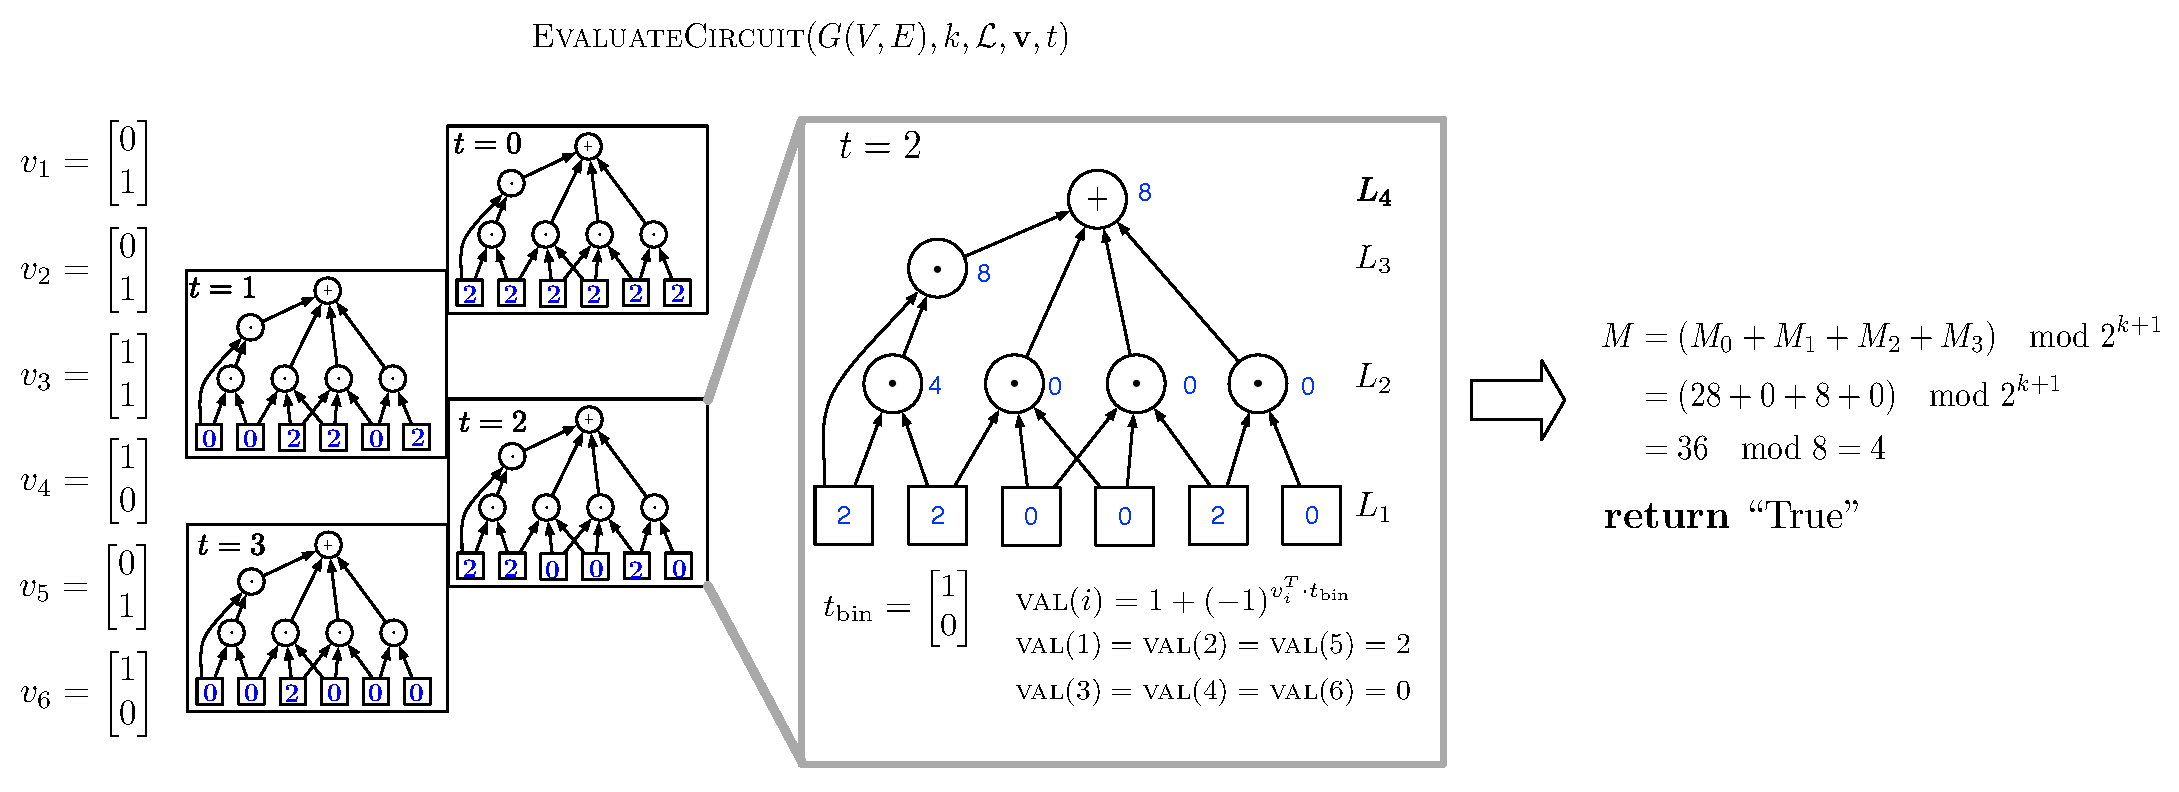
\includegraphics[width=\textwidth]{img/algorithm-example-v2_fixed.pdf}
%%%\caption{
%%%\small
%%%Example of the sequential algorithm \maxwt{}. The input is the circuit $G(V,E)$ from
%%%Figure \ref{fig:dag} with 12 nodes on four levels, $L_1$, $L_2$, $L_3$ and $L_4$, as shown.
%%%The algorithm picks the vectors $v_1,\ldots,v_6$ from $\mathbb{Z}_2^2$, as shown in
%%%the left of the figure. Since $k=2$, there are $2^k=4$ iterations, corresponding to
%%%$t=0,\ldots,3$. The values of $\val(v)=1+(-1)^{v^Tt_{bin}}$ for the $t$th iteration
%%%are shown in blue as the input values. The outputs of the circuit are $M_0, \ldots, M_3$,
%%%with values as shown in the right of the figure. For these choices of the $v_i$'s, the
%%%computed value $M\neq 0 (\text{mod } 2^{k+1})$, which implies the existence of a
%%%multilinear term with $k$ variables. This is true because the term $x_5x_6$ in the
%%%polynomial is indeed multilinear.
%%%%---IDs are in red---$k=2$, and 3 levels. Nodes 1 through 6 are the first level---i.e., the circuit inputs. Nodes 7 through 10 are the second level, all with multiplication operation ($op(i) = \cdot$). The last level only contains the root of the circuit, with addition operation. First, the algorithm generates random vectors $v_i$ for the circuit inputs (bottom left). Then, the circuit is evaluated $2^k$ times by calling procedure \algcircuit{} (center). We show the evaluation for iteration $t=2$. First, we compute the inputs to the circuit as $1 + (-1)^{v_i^T\cdot t_{\text{bin}}}$---this will always be either 2 or 0. From there, we can evaluate the circuit by levels. Finally, back in \maxwt{}, we aggregate the value at root$(G)$ over all the iterations (right). In this case, the polynomial evaluates to $0$, so we return ``False".
%%%%\vspace{-0.2in}
%%%}
%%%\label{fig:algorithm-example}
%%%\end{figure*}

%\begin{algorithm}{}
%\small
%\caption{\maxwt{}$(G(V, E), k$.}
%\label{alg:multilinear-detect}
%\begin{algorithmic}[1]
%\STATE \textbf{Input}: Graph $G(V, E)$, parameter $k$
%\STATE\textbf{Output}: ``True" if circuit evaluation is non-zero. ``False" otherwise.
%\STATE \textbf{Initialize circuit inputs}
%\STATE \textbf{for} node $i \in L_1$ \textbf{do}
%\STATE \quad Let $v_i$ be a random vector from $\mathbb{Z}_{2}^k$
%\STATE \textbf{Initialize the polynomial}
%\STATE Let $M = \bar 0$
%\STATE \textbf{Evaluate circuit for each row of matrix representation}
%\STATE \textbf{for} $t = 0$ to $2^{k-1}$ \textbf{do}
%\STATE \quad $M_t = \algcircuit(G(V, E), k, \mathcal{L}, \mathbf{v}, t)$
%\STATE $M = \sum_{t=0}^{2^{k-1}} M_t \mod 2^{k+1}$
%\STATE \textbf{return} $M \neq 0$
%\STATE
%\STATE \textbf{procedure} \algcircuit{$(G(V, E), k, \mathcal{L}, \mathbf{v}, t)$}
%\STATE \textbf{Input}: Circuit $G(V, E)$, parameter $k$, node levels $\mathcal{L}$, random assigment $\mathbf{v}$, and iteration number $t$
%\STATE\textbf{Output}: Value at root node of $G(V,E)$
%\STATE \textbf{Initialize circuit inputs}
%\STATE \textbf{for} node $i \in L_1$ \textbf{do}
%\STATE \quad $ \val(i) = 1 + (-1)^{v_i^T \cdot t_{\text{bin}}}$
%
%\STATE \textbf{Evaluate the circuit by levels}
%\STATE \textbf{for} $s=2$ to $|\mathcal{L}|$ \textbf{do}
%\STATE \quad \textbf{for} $i \in L_s$ \textbf{do}
%\STATE \qquad \textbf{if} $\op(i) = +$ \textbf{then}
%\STATE \qquad \quad $\val(i) = 0$
%\STATE \qquad \quad \textbf{for} $j \in \pred(i)$ \textbf{do}
%\STATE \qquad \qquad $\val(i) = \val(i) + \val(j)$
%\STATE \qquad \textbf{else} 
%\STATE \qquad \quad $\val(i) = 1$
%\STATE \qquad \quad \textbf{for} $j \in \pred(i)$ \textbf{do}
%\STATE \qquad \qquad $\val(i) = \val(i) \cdot \val(j)$
%
%\STATE \textbf{return} $\val($root$(G))$
%\end{algorithmic}
%\end{algorithm}

%\begin{algorithm}{}
%\small
%\caption{\small \textsc{MLD-ScanStat}$(G(V, E), \mathbf{w}, k, \epsilon, r)$.}
%\label{alg:mld-scanstat}
%\begin{algorithmic}[1]
%\STATE \textbf{Input}: Instance $(G(V, E), \mathbf{w})$ and parameters $k, \epsilon, r$
%\STATE\textbf{Output}: "True" if $G$ has a subgraph $S$ with size $i \leq k$ and weight $j \leq r$
%\STATE Let $K=\{1,\ldots,k\}, R=\{0, \ldots, r\}$
%\STATE \textbf{Initialize the polynomial}
%\STATE $P(i, j) = \bar{0}$ for $i \in K$, $j \in R$
%\STATE For each node $v$, pick a random vector $x_v \in Q[\mathbb{Z}_{2}^k]$
%\STATE \textbf{Evaluate the circuit for each row of matrix representation}
%\STATE \textbf{for} $t = 0$ to $2^{k-1}$
%\STATE \quad $P_v(i, j) = \bar{0}$ for $i \in K$, $j \in R$
%\STATE \quad \textbf{Initialize circuit inputs}
%\STATE \quad \textbf{for} $v \in V$ \textbf{do}
%\STATE \quad \quad $P_v(1, w(v)) = 1 + (-1)^{x_v^T \cdot t_{\text{bin}}}$
%\STATE \quad \textbf{Evaluate circuit recursively}
%\STATE \quad \textbf{for} $v \in V$, $i = 2$ to $k$, $j = 0$ to $r$ \textbf{do}
%\STATE \qquad $P_v(i,j) = \sum_{u \in \nbr(v)} \sum_{i' = 1}^{i-1}\sum_{j'=0}^j (P_v(i', j') \cdot P_u(i-i', j - j'))$ 
%\STATE
%\STATE \textbf{return} $P \neq \bar 0$
%\end{algorithmic}
%\end{algorithm}

\begin{algorithm}{}
\small
\caption{\parcircuitscan{$(G(V, E), k, \textbf{w}, \mathbf{v}, t, N_2, N_1, \mathcal{P})$}}
\label{alg:parEvaluateScanStat} 
\begin{algorithmic}[1]
\STATE \textbf{Input:} Graph $G(V, E)$, parameter $k$, node weights $\mathbf{w}$, 
random assignment $\mathbf{v}$, phase number $t$, number of iterations within phase $N_2$,
number of partitions $N_1$, and partitioning $\mathcal{P}$
\STATE \textbf{Output:} The value of the polynomial corresponding to the scan statistics in the iterations within a phase
\STATE
\STATE \textbf{for} each processor $s$ \textbf{do in parallel}
\STATE \quad \textbf{for} node $i \in G^s$ and iteration $q \in [tN_2,(t+1)N_2-1]$ \textbf{do}
\STATE \qquad $ P(i, q, 1, w(v)) = 1 + (-1)^{v_i^T \cdot q_{\text{bin}}}$
\STATE \quad \textbf{for} $j=2$ to $k$ and $z=0$ to $W(V)$ \textbf{do}
\STATE \qquad \textbf{for} node $i \in G^s$ \textbf{do}
\STATE \qquad \quad \textbf{for} all $q$ set $P(i,q, j, z) = 0$
\STATE \qquad \quad \textbf{for} each incoming message $\langle u, P(u, q, j-j', z-z')\rangle$ \textbf{do}
\STATE \qquad \qquad $P(i, q, j, z)= P(i, q, j, z) + P(i, q, j', z')  P(u, q, j-j', z-z')$
\STATE \qquad \quad  \textbf{Send result to neighbors}
\STATE \qquad \quad \textbf{for} $u \in \nbr(i)\setminus G^s$ \textbf{do}
\STATE \qquad \qquad \textbf{Send} $\langle i, P(i, q, j, z)\rangle$
\STATE \textsc{MpiBarrier}
\STATE \textbf{return} $\sum_q \sum_i P(i, q, k, z)$ for all $z \leq W(V)$
\end{algorithmic}
\end{algorithm}
% !TEX root = ./multilinear.tex
\section{Experiments}
\label{sec:experiments}
The experimental study of the proposed parallel algorithms covers the following topics.

\begin{itemize}
\item
\textbf{Effect of partition size.} We analyze performance with partition size as $N_1$ is varied (Section~\ref{sec:perf-part-size}).

\item
\textbf{Scalability with subgraph size.} We depict the total runtime as subgraph size is increased (Section \ref{sec:perf-subgraph-size}).

\item 
\textbf{Strong scaling.} We show the total runtime as the number of parallel processors is increased, thereby reducing the computing workload per process (Section \ref{sec:perf-strong-scaling}).

\item
\textbf{\ouralgo{} vs. FASCIA.} We present the runtime of our implementation compared to FASCIA (Section~\ref{sec:perf-vsfasci}).

\item
\textbf{Scan Statistics and its applications.} We provide performance results for the parallel scan statistics algorithm and present an application (Section \ref{sec:perf-scan-stat}).

\end{itemize}

\subsection{Experimental Setup}
\subsubsection{Hardware}
Experiments were conducted on Juliet, an Intel Haswell HPC cluster. Up to 32 nodes were used for the evaluation, where each node has 36 cores (2 sockets $\times$ 18 cores each). A node consists of 128GB of main memory and 56Gbps Infiniband interconnect. We also tested on another HPC cluster, Shadowfax-Haswell, where we used 32 nodes each with 32 cores (2 sockets $\times$ 16 cores each). Memory and interconnect of this cluster are similar to those of Juliet.

\subsubsection{Datasets}
We evaluate our algorithms on two large graphs: 1) a social contact network of Miami, commonly used in agent-based simulation studies \cite{barrett2009generation}, and 2) a snapshot of the Orkut social network\footnote{\url{https://snap.stanford.edu/data/com-Orkut.html}}. In addition, we perform experiments in two Erdos-Renyi networks of 1 and 10 million nodes with an expected number of edges of $n\log n$, where $n$ is the number of nodes. A summary of the datasets is provided in Table \ref{table:datasets}.

\begin{table}[ht]
\centering \caption{\small Datasets used in our experiments}
\vspace{-.1in}
\label{table:datasets}
%\resizebox{\columnwidth}{!}{
%\begin{scriptsize}
\begin{tabular}{|l|r|r|}
\hline
\textbf{Dataset}  & \textbf{Nodes ($\times 10^6$)} & \textbf{Edges ($\times 10^6$)} \\
\hline
miami & 2.1 & 51.5\\
\hline
com-Orkut  & 3.1 & 234.3\\
\hline
random-1e6 & 1 & 13.8\\
\hline
random-1e7 & 10 & 161.8\\
\hline
\end{tabular}
%\end{scriptsize}
%}
\end{table}

\begin{figure*}[!htb]
    \centering
    \begin{minipage}{0.32\textwidth}
        \centering        
        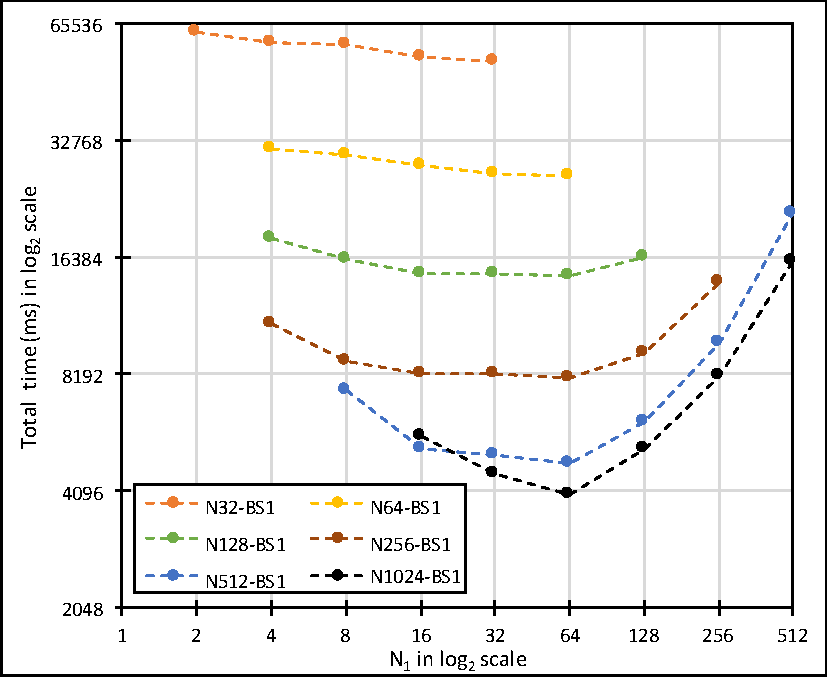
\includegraphics[width=1\columnwidth]{img/kpath-N1N/fig-perf-kpath-1mil-k6-bs1.pdf}
        \caption{$k$-path total runtime for random-1e6 and varying $N_1$. Note. $BS1=N_2=1$}
        \label{fig:fig-perf-kpath-1mil-k6-bs1.pdf}
    \end{minipage}
    \hspace{0mm}
    \begin{minipage}{0.32\textwidth}
        \centering
        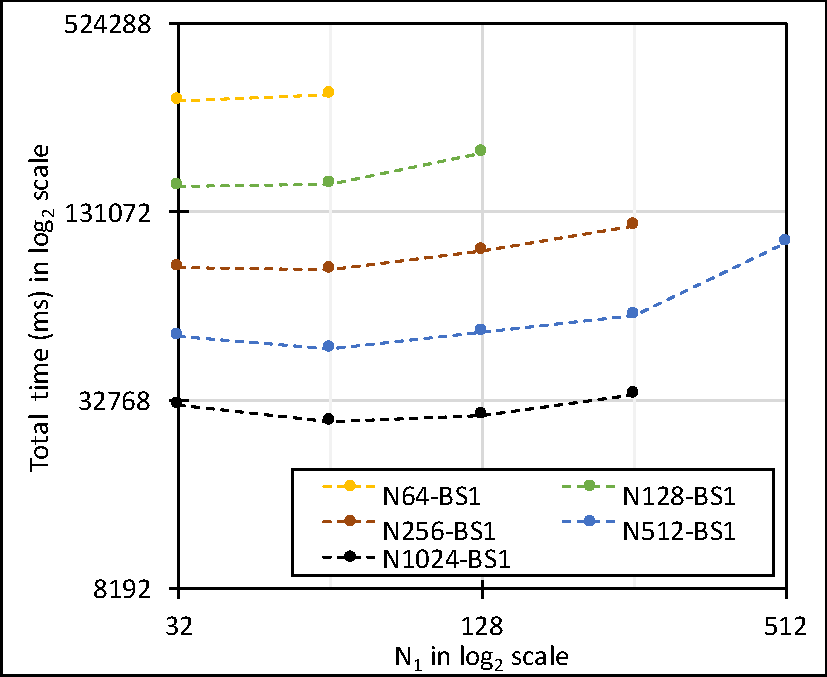
\includegraphics[width=1\columnwidth]{img/kpath-N1N/fig-perf-kpath-orkut-k6-bs1.pdf}
        \caption{$k$-path total runtime for com-Orkut and varying $N_1$. Note. $BS1=N_2=1$}
        \label{fig:fig-perf-kpath-orkut-k6-bs1.pdf}
    \end{minipage}  
    \hspace{0mm}
    \begin{minipage}{0.33\textwidth}
        \centering
        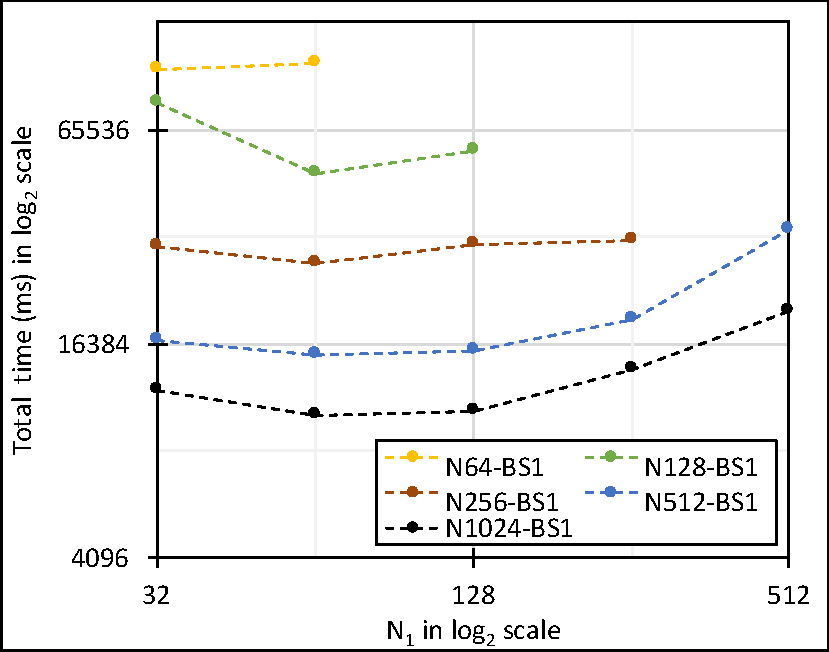
\includegraphics[width=1\columnwidth]{img/kpath-N1N/fig-perf-kpath-miami-k6-bs1.pdf}
        \caption{$k$-path total runtime for miami and varying $N_1$. Note. $BS1=N_2=1$}
        \label{fig:fig-perf-kpath-miami-k6-bs1.pdf}
    \end{minipage}  
\end{figure*}

\begin{figure*}[!htb]
    \centering
    \begin{minipage}{0.32\textwidth}
        \centering        
        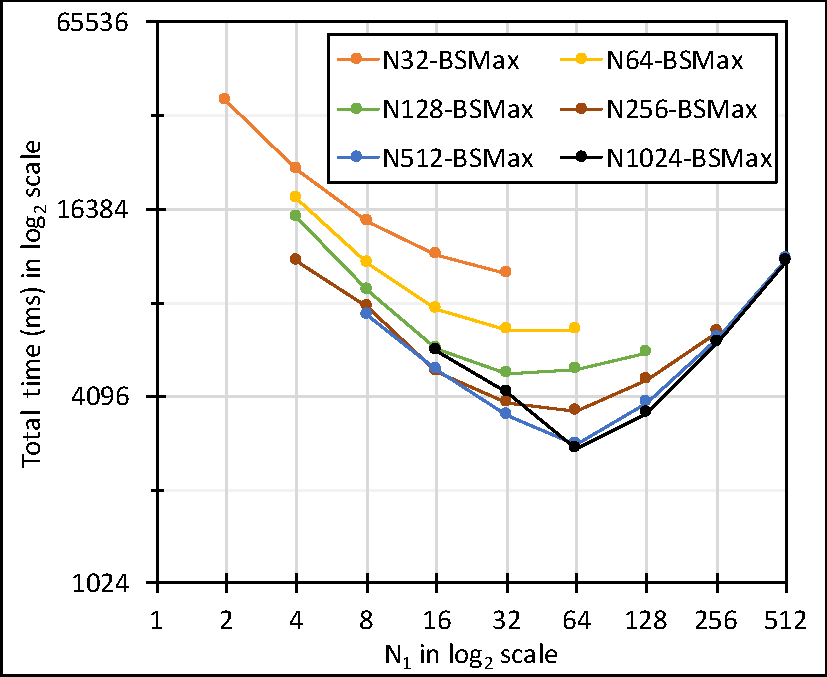
\includegraphics[width=1\columnwidth]{img/kpath-N1N/fig-perf-kpath-1mil-k6-bsmax.pdf}
        \caption{$k$-path total runtime for random-1e6 and varying $N_1$. Note. $BSMax=N_2=2^kN_1/N$}
        \label{fig:fig-perf-kpath-1mil-k6-bsmax.pdf}
    \end{minipage}
    \hspace{0mm}
    \begin{minipage}{0.32\textwidth}
        \centering
        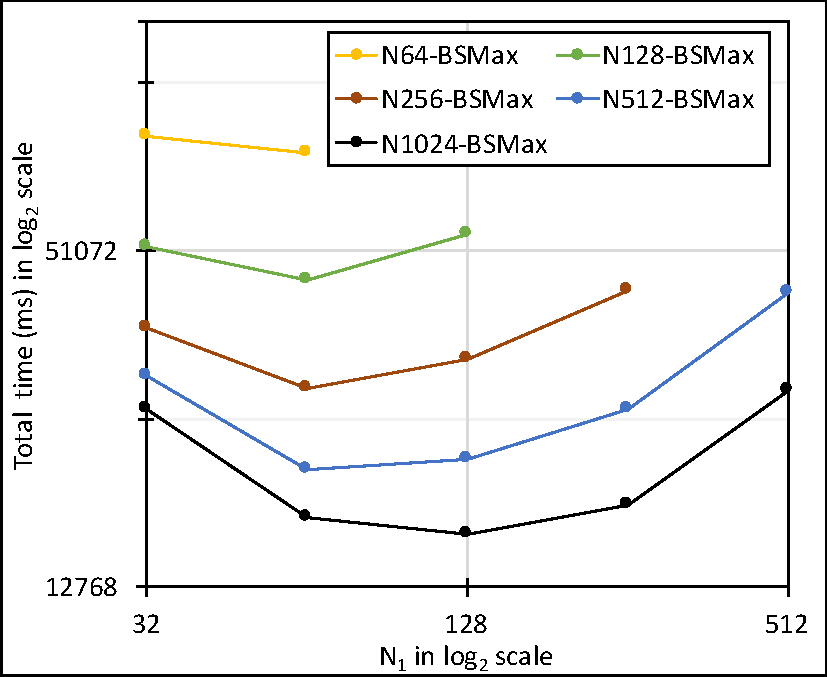
\includegraphics[width=1\columnwidth]{img/kpath-N1N/fig-perf-kpath-orkut-k6-bsmax.pdf}
        \caption{$k$-path total runtime for com-Orkut and varying $N_1$. Note. $BSMax=N_2=2^kN_1/N$}
        \label{fig:fig-perf-kpath-orkut-k6-bsmax.pdf}
    \end{minipage}  
    \hspace{0mm}
    \begin{minipage}{0.32\textwidth}
        \centering
        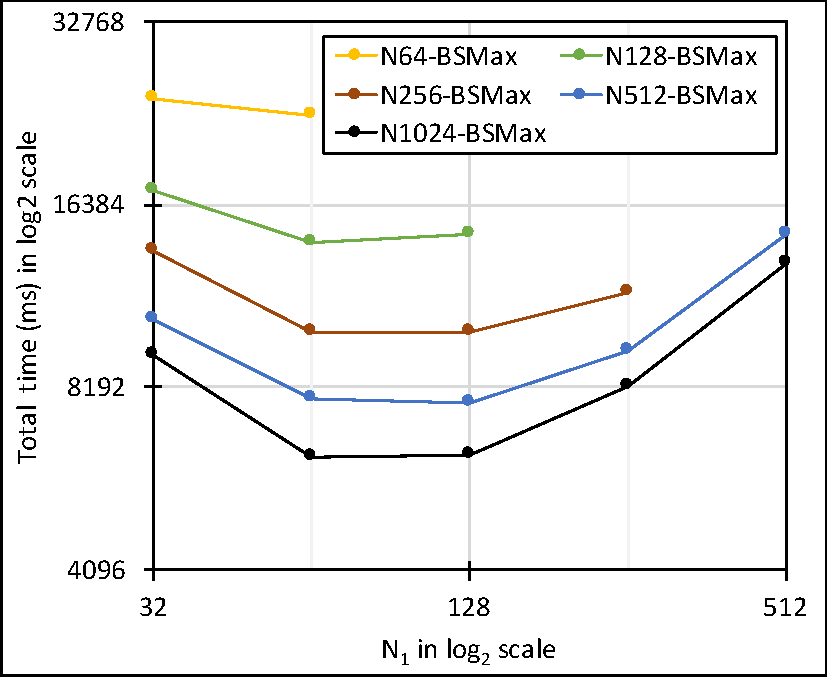
\includegraphics[width=1\columnwidth]{img/kpath-N1N/fig-perf-kpath-miami-k6-bsmax.pdf}
        \caption{$k$-path total runtime for miami and varying $N_1$. Note. $BSMax=N_2=2^kN_1/N$}
        \label{fig:fig-perf-kpath-miami-k6-bsmax.pdf}
    \end{minipage}  
\end{figure*}

% [Saliya] I think we don't need this section on
% independence of iterations because now we don't
% run these as separate instances. Everything is 
% automatically done within the program.
% \subsection{Independence of Iterations}
% \label{sec:independence}
% First, we examine the extent to which the $2^k$ iterations of the outer loop in
% Algorithm \parmaxwt{} are independent and take the same time. Figure \ref{fig:indep} shows the running time as the number of processors $N$ is increased for the random network of 1 million nodes. This figure implies that the running time is almost invariant with the
% number of parallel iterations that are run simultaneously. We observed similar results with com-Orkut graph as shown in Figure~\ref{fig:indep-orkut}. We use this insight to estimate the total running time for other settings. 

% \begin{figure}[!htpb]
% 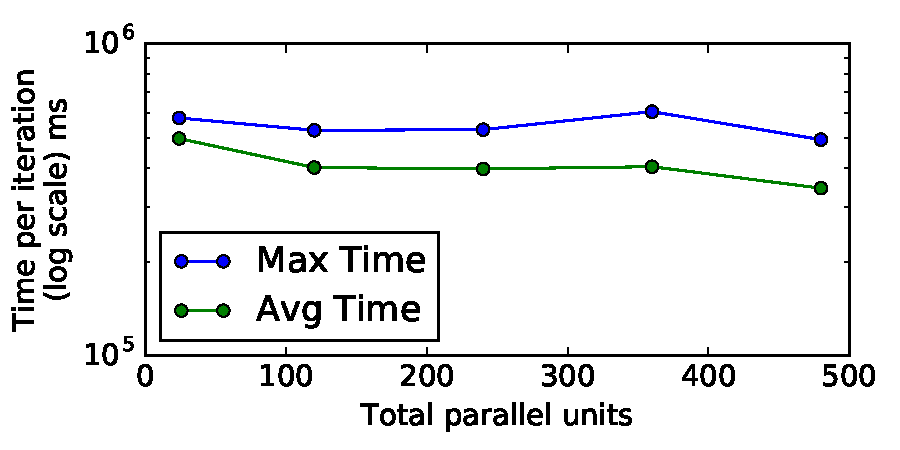
\includegraphics[width=0.4\textwidth]{img/fig-random-1mil-timeperiteration.pdf}
% \caption{Time per iteration with varying parallel units for random 1 million nodes network.}
% \label{fig:indep}
% \end{figure}

% \begin{figure}[!htpb]
% 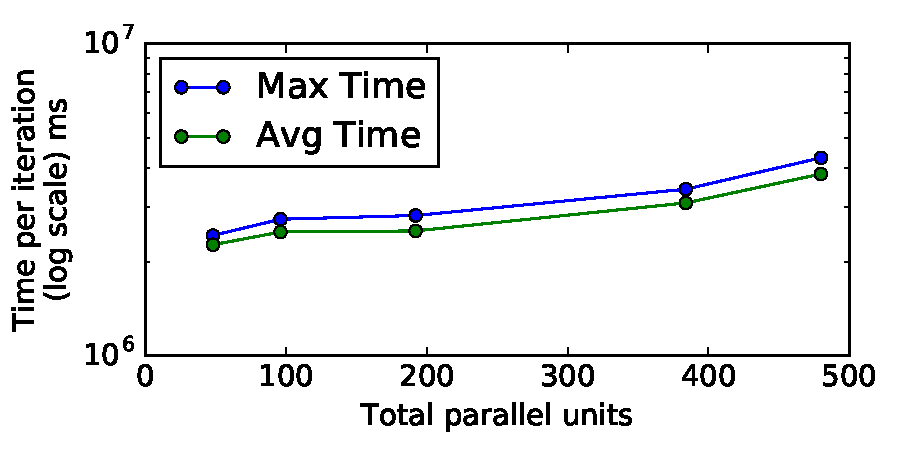
\includegraphics[width=0.4\textwidth]{img/fig-orkut-timeperiteration.pdf}
% \caption{Time per iteration with varying parallel units for Orkut network.}
% \label{fig:indep-orkut}
% \end{figure}

\subsection{Effect of partition size}
\label{sec:perf-part-size}
Our parallel $k$-Path algorithm exhibits two levels of parallelism: vertex and iterations. On one hand, the $2^k$ iterations are pleasingly parallel except for a global reduction at the end. The parallel vertex computation within each iteration, on the other hand, requires message passing between neighbors for $k-1$ steps---in the case of trees, this would be the number of sub-templates instead of $k-1$. 

% \textcolor{blue}{TODO - change bs to N2}

Given these two levels of parallelism and a total of $N$ processes, we can split the $2^k$ iterations among $a=N/N_1$  parallel phases. Each phase decomposes the graph across $N_1$ processes and performs the $k$-Path computation in parallel for $2^k/a$. To reduce the communication over computation cost, the algorithm packs a user defined $N_2$ number of iterations into one computation step, so each parallel phase only has to perform $ 2^k/(a*N_2)$ compute and communication phases. 
To illustrate this with an example, consider the case of $k=6$, $N=128$, $N_1=32$, and $N_2=8$. The total number of iterations is $2^k = 64$. The number of parallel phases corresponding to $N_1=32$ is $128/32 = 4$. Each phase only needs to run $64/4 = 16$ iterations. Since $N_2=8$, the $16$ iterations can be completed in just $16/8 = 2$ batches.

Increasing $N_2$, for example $N_2=16$ in the previous case, would allow us to finish the entire program in one compute and communicate batch. This results in higher parallel efficiency as the overhead of communication to computation is reduced. However, it increases the message size by a factor of $N_2$\footnote{Increasing message size for a communication step is not necessarily bad. Reducing the number of small messages in communication may lead to increased network performance\cite{smallmessagecoalasce}.}. Depending on the number of total processes, MPI may fail to accommodate very large message sizes requiring to reduce $N_2$, so that some form of chunking method may be required. 

%We evaluate the total time to complete for $k$-Path and scan statistics as a function of $N_1$, the number of processes used to run 
%each of the $2^k$ circuit evaluations. Figure \ref{fig:time-with-p} shows the total time for both applications varying $N$ and $N_1$. First, we note that, as $N$ becomes larger, the total running time decreases for all values of $N_1$, which is expected. Second, we obtain the best performance by assigning around 8 parallel units to process an iteration, regardless of the total parallel units.

% Figure 3 and Figure 6 --> As N1 increase message parallalization of compute regions increase, but this also increase number of communication steps. 
% For N2 = 1
Figures~\ref{fig:fig-perf-kpath-1mil-k6-bs1.pdf}, \ref{fig:fig-perf-kpath-orkut-k6-bs1.pdf}, \ref{fig:fig-perf-kpath-miami-k6-bs1.pdf} show the performance of \ouralgo{} on three different datasets when $N_2=1$. We observe that running times of \ouralgo{} when $N_2$ is scaled for a fixed value of $N$ for each problem size---this effectively tested our parallel algorithm for a large range of configurations. Our observations confirm the existence of an optimal point (i.e., a minimum) between the two levels of parallelism discussed before. The communication cost gradually increases when moving from one extreme end of parallelism to the other because of the increase in number of messages exchanged \footnote{Number of messages exchanged can be approximated to $O(\log{N_1})$ for small message sizes where $N_1$ ranges from $N_1=1$ to $N_1\rightarrow N$}. However, at the optimal point, the cost of communication can be sufficiently amortized by the amount of parallelism gained. In other words, the optimal setting for \ouralgo{} can be found in a point between vertex level and iteration based parallelism. 

The observed speedup (1x to 2x) is due to cache affinity effects on the main loop and reduction of communication phases by increasing the message size.
Interestingly, when $N_2$ is increased (Figures~\ref{fig:fig-perf-kpath-1mil-k6-bsmax.pdf}, \ref{fig:fig-perf-kpath-orkut-k6-bsmax.pdf}, \ref{fig:fig-perf-kpath-miami-k6-bsmax.pdf}) we observe further relative performance gains on the same set of experiments. Furthermore, speedups are evident for each experiment instance of the $k$-path problem when problem size is scaled. As a general guideline, we find that keeping $N_1$ close to the number of cores in one or two machines lead to better performance. A more formal characterization of the trade-off between $N_1$ and $N_2$ is a topic for future work.


\begin{figure*}[!htb]
    \centering
    \begin{minipage}{0.29\textwidth}
        \centering        
        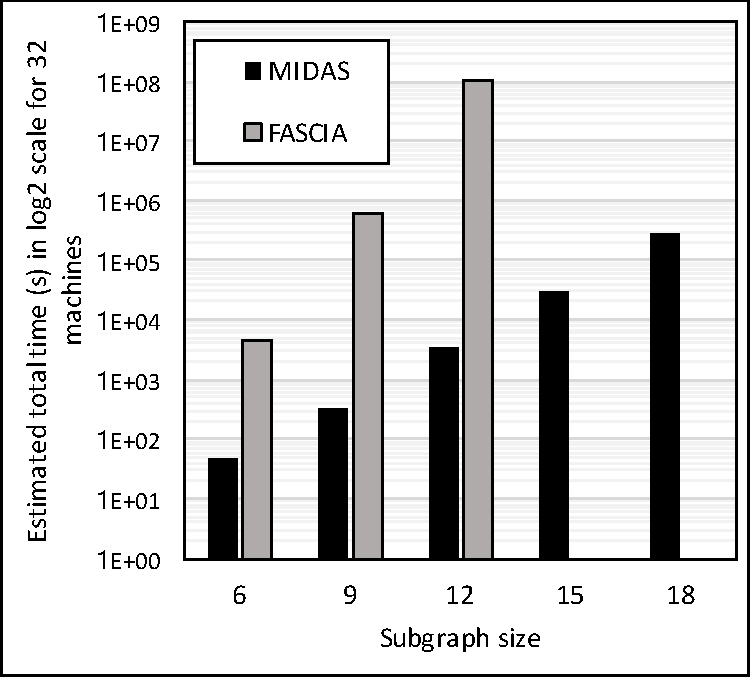
\includegraphics[width=1\columnwidth]{img/fig-perf-vsfascia.pdf}
        \caption{\ouralgo{} runtime compared to FASCIA for varying subgraph sizes in the $k$-path problem}
        \label{fig:fig-perf-vsfascia.pdf}
    \end{minipage}
    \hspace{0mm}
    \begin{minipage}{0.32\textwidth}
        \centering        
        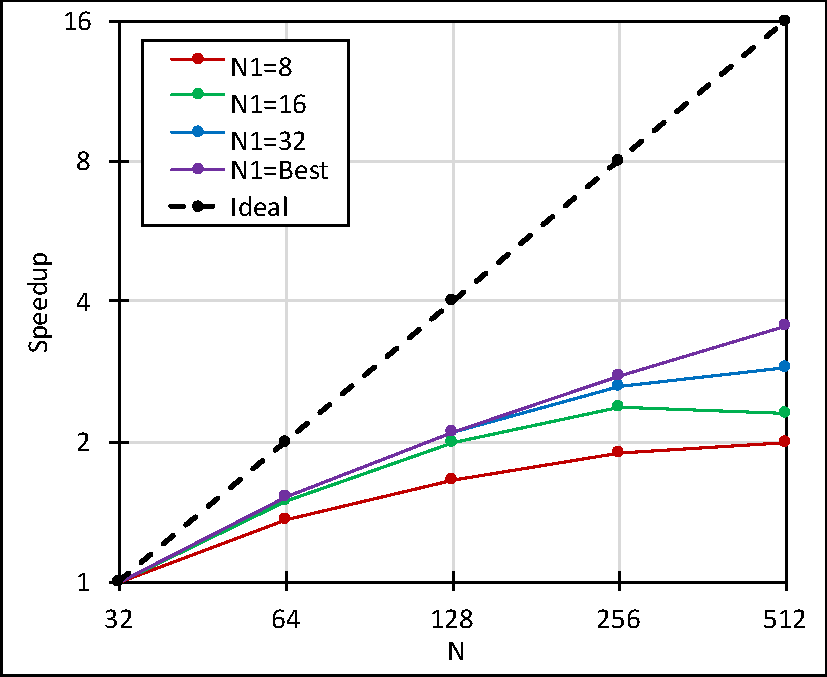
\includegraphics[width=1\columnwidth]{img/kpath-N1N/fig-perf-kpath-1mil-speedup-N1fixed.pdf}
        \caption{\ouralgo{} strong scaling for the $k$-path problem with increasing $N$, while $N_1$ is fixed.}
        \label{fig-perf-kpath-1mil-speedup-N1fixed.pdf}
    \end{minipage}
    \hspace{0mm}
    \begin{minipage}{0.32\textwidth}
        \centering        
        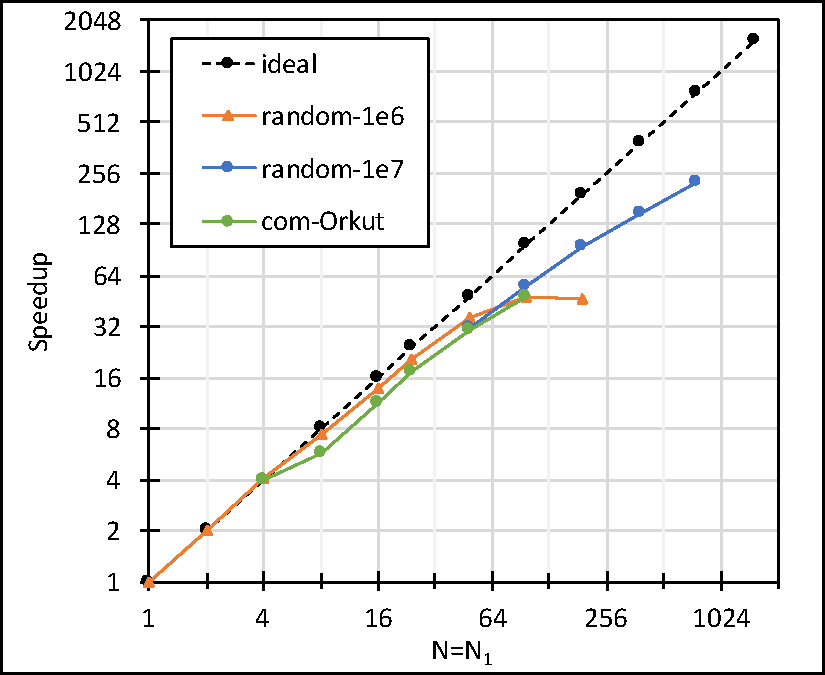
\includegraphics[width=1\columnwidth]{img/kpath-N1N/fig-perf-kpath-speedup-N=N1.pdf}
        \caption{\ouralgo{} strong scaling for the $k$-path problem with increasing $N$ and $N_1=N$}
        \label{fig:fig-perf-kpath-speedup-N=N1.pdf}
    \end{minipage}
\end{figure*}

\begin{figure*}[!htb]
    \centering
    \begin{minipage}{0.32\textwidth}
        \centering        
        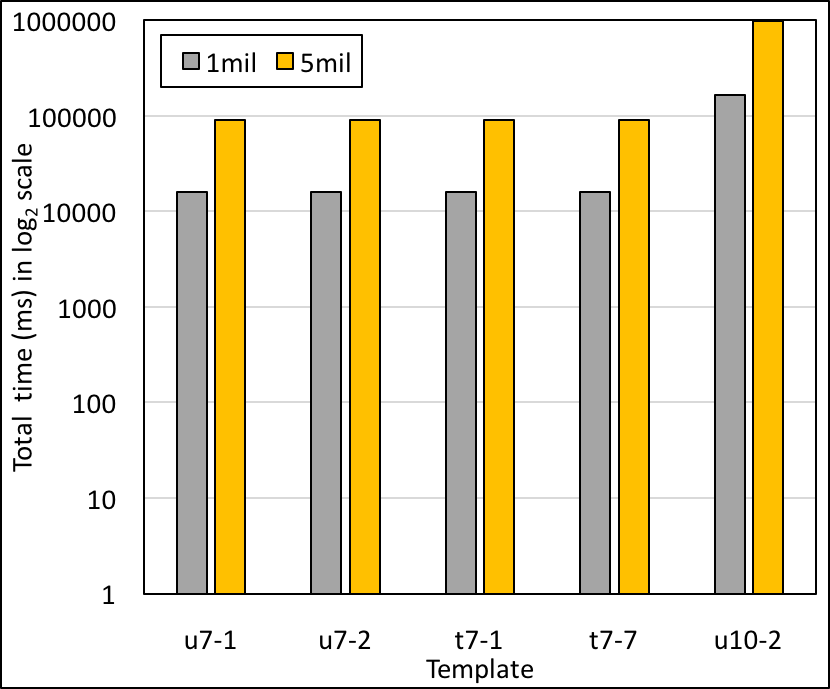
\includegraphics[width=1\columnwidth]{img/ktree/ktree-1mil-5mil-16nodes.png}
        \caption{$k$-tree total runtime for random 1e6 and 5e6 for different templates. Note. $N=16$}
        \label{fig:ktree-1mil-5mil-16nodes.png}
    \end{minipage}
    \hspace{0mm}
    \begin{minipage}{0.32\textwidth}
        \centering        
        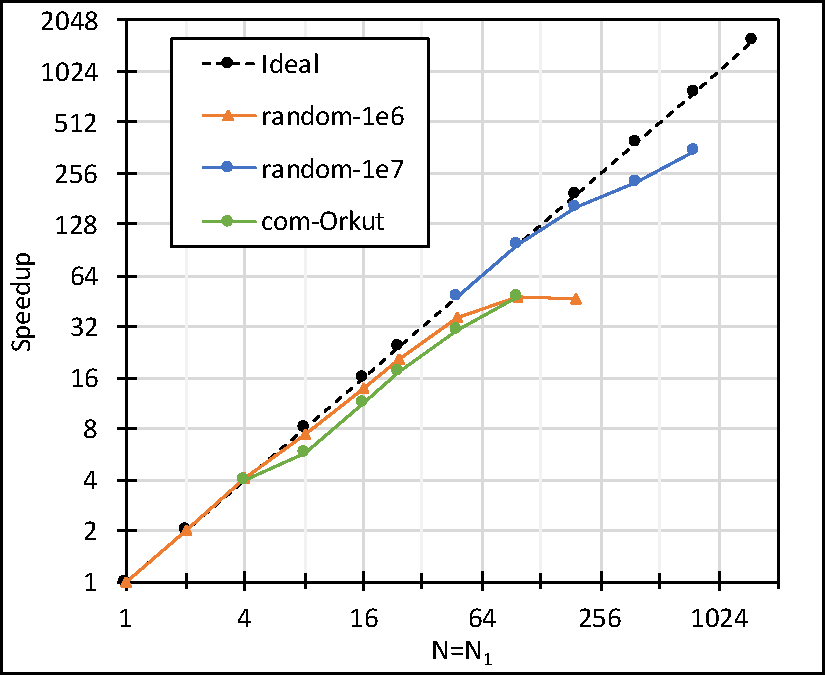
\includegraphics[width=1\textwidth]{img/fig-perf-scan-speedup-N=N1.pdf}
        \caption{\ouralgo{} strong scaling for the scan statistics problem with increasing $N$ and $N_1=N$}
        \label{fig:fig-perf-scan-speedup-N=N1.pdf}
    \end{minipage}  
    \hspace{0mm}
    \begin{minipage}{0.32\textwidth}
        \centering
        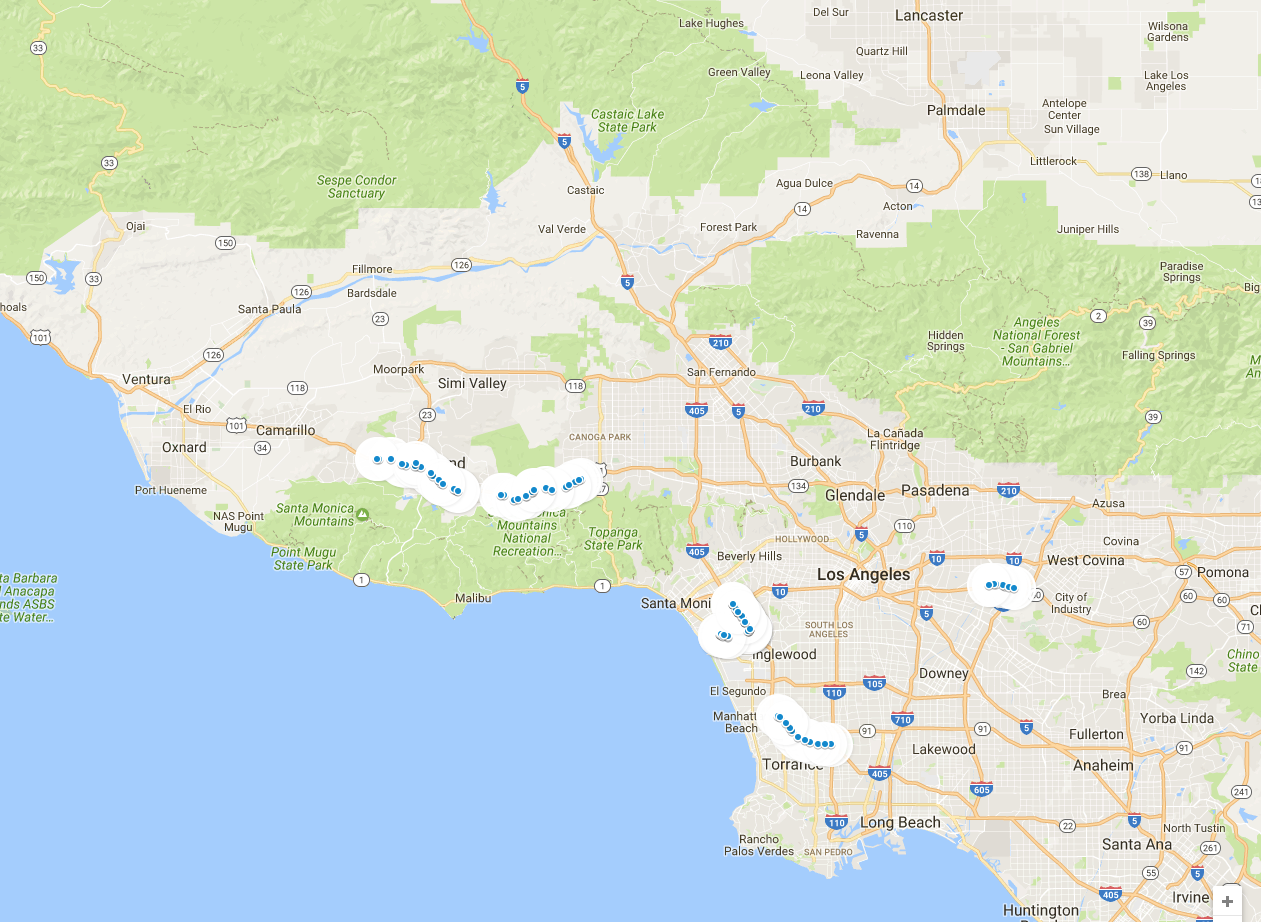
\includegraphics[width=1\textwidth]{img/traffic-example.png}
        \caption{Discovering highway segments with unexpected congestion in the Los Angeles road network.}
        \label{fig:traffic}
    \end{minipage}  
\end{figure*}

% \begin{figure*}[!htb]
%     % \centering
%     \begin{minipage}{0.2\textwidth}
%         \centering        
%         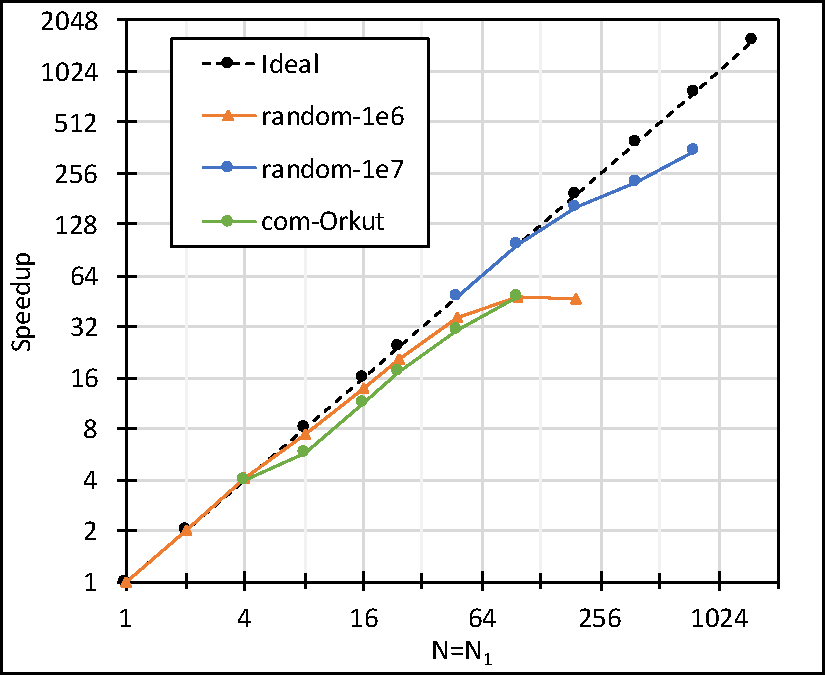
\includegraphics[width=1\columnwidth]{img/fig-perf-scan-speedup-N=N1.pdf}
%         \caption{\ouralgo{} strong scaling for the Scan Statistics problem with increasing $N$ and $N_1=N$}
%         \label{fig:fig-perf-scan-speedup-N=N1.pdf}
%     \end{minipage}
%     \hspace{0mm}
%     \begin{minipage}{0.2\textwidth}
%         \centering
%         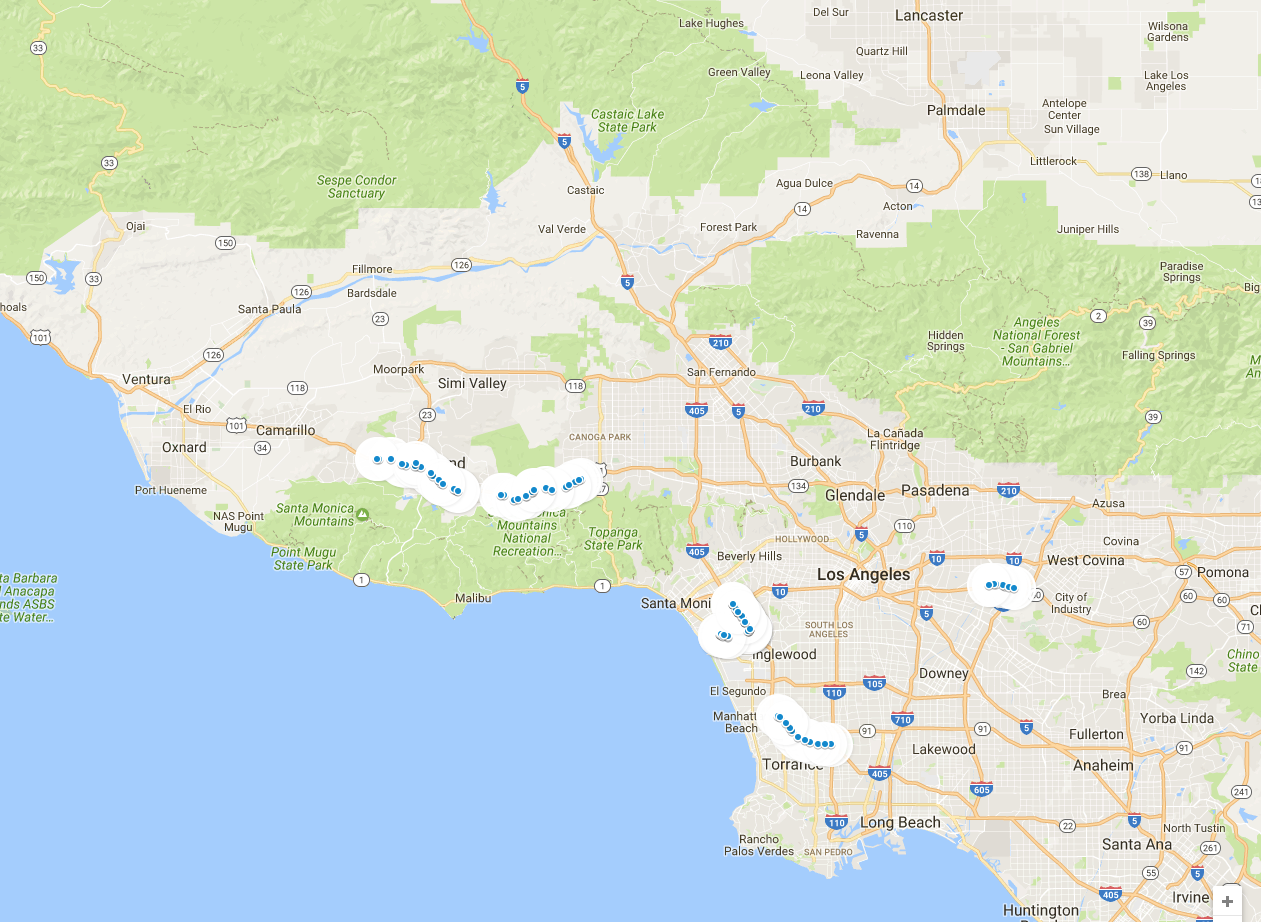
\includegraphics[width=1\columnwidth]{img/traffic-example.png}
%         \caption{Discovering highway segments with unexpected congesion in the Los Angeles road network.}
%         \label{fig:traffic}
%     \end{minipage}
% \end{figure*}

% \begin{figure}
%     \centering        
%     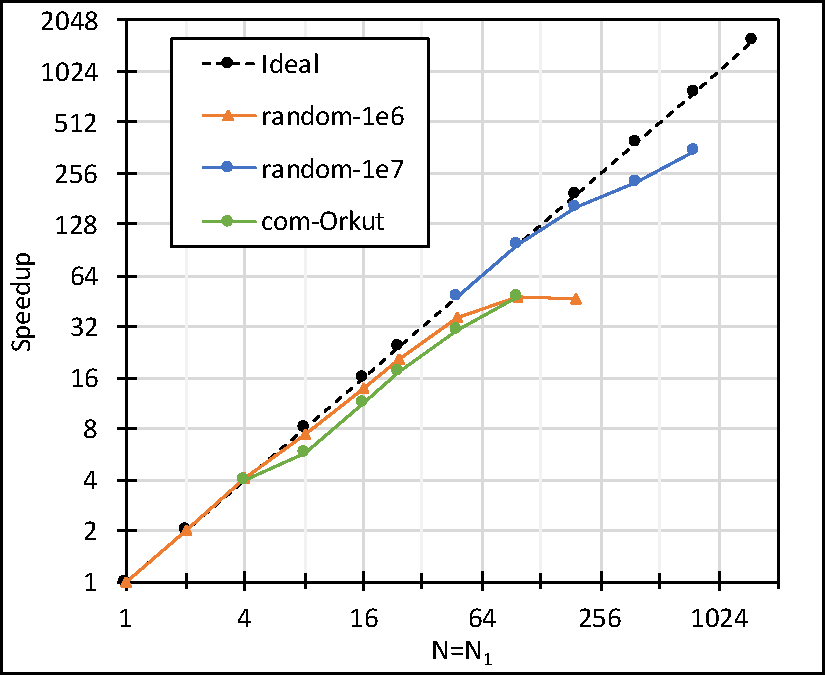
\includegraphics[width=0.6\columnwidth]{img/fig-perf-scan-speedup-N=N1.pdf}
%     \caption{\ouralgo{} strong scaling for the Scan Statistics problem with increasing $N$ and $N_1=N$}
%     \label{fig:fig-perf-scan-speedup-N=N1.pdf}
% \end{figure}

% \begin{figure}
%     \centering
%     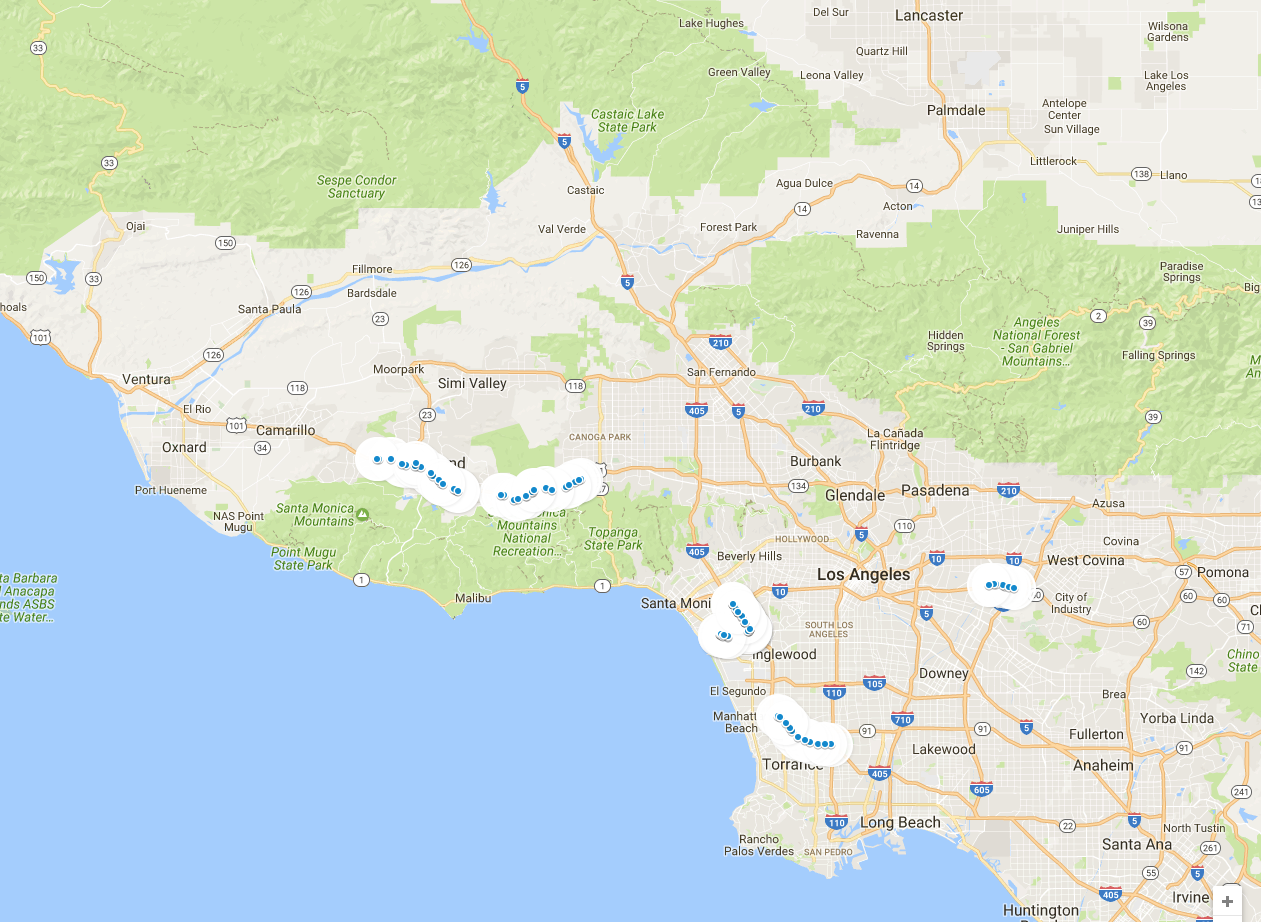
\includegraphics[width=0.6\columnwidth]{img/traffic-example.png}
%     \caption{Discovering highway segments with unexpected congesion in the Los Angeles road network.}
%     \label{fig:traffic}
% \end{figure}


\subsection{Scalability with subgraph size}
\label{sec:perf-subgraph-size}
In Figure~\ref{fig:fig-perf-vsfascia.pdf}, we increase the subgraph size, $k$, in both FASCIA and \ouralgo{}, while keeping $N$ and $N_1$ fixed. Figures~\ref{fig:fig-perf-kpath-1mil-k6-bsmax.pdf}--\ref{fig:fig-perf-kpath-miami-k6-bsmax.pdf} suggest it is best to keep $N_2$ as high as possible to leverage the cache locality benefits discussed above. However, the total message size communicated out of a process increases with $N_2$ leading to diminishing returns. Therefore, we've kept $N_2<1024$. %The results in Figure~\ref{fig:fig-perf-scan-speedup-N=N1.pdf} verifies the total runtime grows exponentially with subgraph size, $k$ in this case.

\subsection{Strong  scaling}
\label{sec:perf-strong-scaling}
The strong scaling of \ouralgo{} can be investigated in two ways. The first is to fix $N_1$ and change $N$, thereby increasing the parallel phases to split the $2^k$ iterations. We could observe the effect of this behavior by examining the values along a fixed $N_1$ value in Figures~\ref{fig:fig-perf-kpath-1mil-k6-bs1.pdf}--\ref{fig:fig-perf-kpath-miami-k6-bsmax.pdf}. Dividing the runtime corresponding to the minimum $N$ (the top most line) by the given $N$ gives speedup indicating the strong scalability of \ouralgo{}. 

Figure~\ref{fig-perf-kpath-1mil-speedup-N1fixed.pdf} presents such speedup for a set of $N_1$ values over varying $N$. We observe the results do not necessarily scale linearly due to the fact that communication within a phase is dominant. We get the best speedup by going along points in Figures~\ref{fig:fig-perf-kpath-1mil-k6-bs1.pdf}--\ref{fig:fig-perf-kpath-miami-k6-bsmax.pdf} that gave the minimum runtime. This is shown as the $N1=\text{Best}$ line in Figure~\ref{fig-perf-kpath-1mil-speedup-N1fixed.pdf}.

The other form of strong scalability we can test is by setting $N1=N$. This produces a single phase and is the classic strong scaling of parallel graph algorithms. Figure~\ref{fig:fig-perf-kpath-speedup-N=N1.pdf} presents the speedup values for different datasets. Even though the speedups are less than ideal, we still observe good performance up to a considerable number of processes.

\subsection{\ouralgo{} vs.\ FASCIA}
\label{sec:perf-vsfasci}
Figure~\ref{fig:fig-perf-vsfascia.pdf} compares the running time of FASCIA to \ouralgo{} for varying subgraph sizes. We see FASCIA fails to support beyond subgraphs of size 12 on the random-1e6 graph, whereas \ouralgo{} scales to well over 18. Also, \ouralgo{} shows a significant improvement over FASCIA in runtime. Figure~\ref{fig:ktree-1mil-5mil-16nodes.png} shows \ouralgo{} performance for different tree templates of random-1e6 and random-5e6. The details of the templates can be found in the FASCIA papers~\cite{slota:icpp13, slota:ipdps14}.

\subsection{Scan statistics optimization}
\label{sec:perf-scan-stat}
In Figure~\ref{fig:fig-perf-scan-speedup-N=N1.pdf}, we present strong scaling results for the scan statistics problem where $N_1$ is set to $N$. We do this for multiple datasets and observe considerable strong scalability similar to the $k$-Path problem in Figure~\ref{fig:fig-perf-kpath-speedup-N=N1.pdf}.

We apply our algorithm for scan statistics to find clusters with unexpectedly low-moving traffic in the highway network of Los Angeles County\footnote{\url{http://pems.dot.ca.gov/}}. Nodes in the graph are sensors next to the road that record the average speed and the number of vehicles passing through. We have 30-minute snapshots for May 2014. We assume that the average speed recorded by each sensor follows a normal distribution. Then, the $p$-value of a node $i$ is the cumulative distribution function of a normal distribution with mean  $\mu_i^{[1,t-1]}$ and standard deviation $\sigma_i^{[1,t-1]}$, where $\mu_i^{[1,t-1]}$ and $\sigma_i^{[1,t-1]}$ are, respectively, the sample mean and standard deviation for node $i$ from snapshots $1$ to $t-1$.

We use our algorithm with $k=12$ on this dataset. In Figure \ref{fig:traffic}, we show with blue dots highway segments that our algorithm identifies as having \emph{unexpectedly} low average speed during rush hour (16:00 to 19:00) on Friday May 9, 2014. These segments are not necessarily the ones with most congestion. For instance, the center of Los Angeles city has higher congestion; however, such activity is normal on Friday afternoons according to the previous snapshots. The clusters shown in the map are selected because they have significantly lower average speeds than in previous observations.  

% \subsection{Strong Scaling and Speedup}
% \label{sec:perf-strong-scaling}
% In Figure \ref{fig:scaling}, we show the speed up and strong scaling achieved by increasing the total parallelism. We obtain higher speed up for $k$-Path, possibly because the communication overhead for this program is lower than for Multilinear Scan. In both cases, we the scaling factor is better for the LiveJournal network.

% \begin{figure*}[ht]
%   \centering
%   \begin{subfigure}[b]{\textwidth}
%     \centering
%     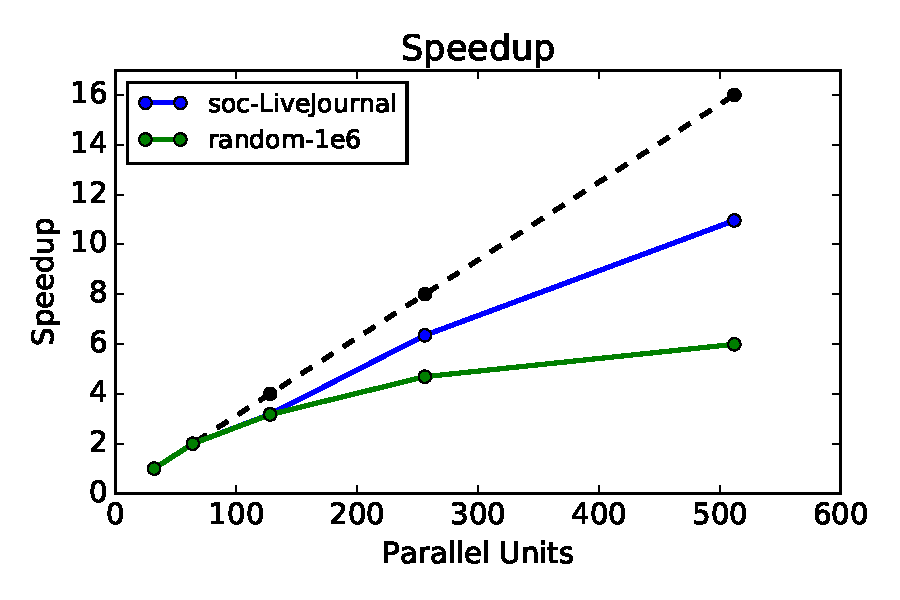
\includegraphics[width=0.45\textwidth]{img/speedup-kpath.pdf}
%     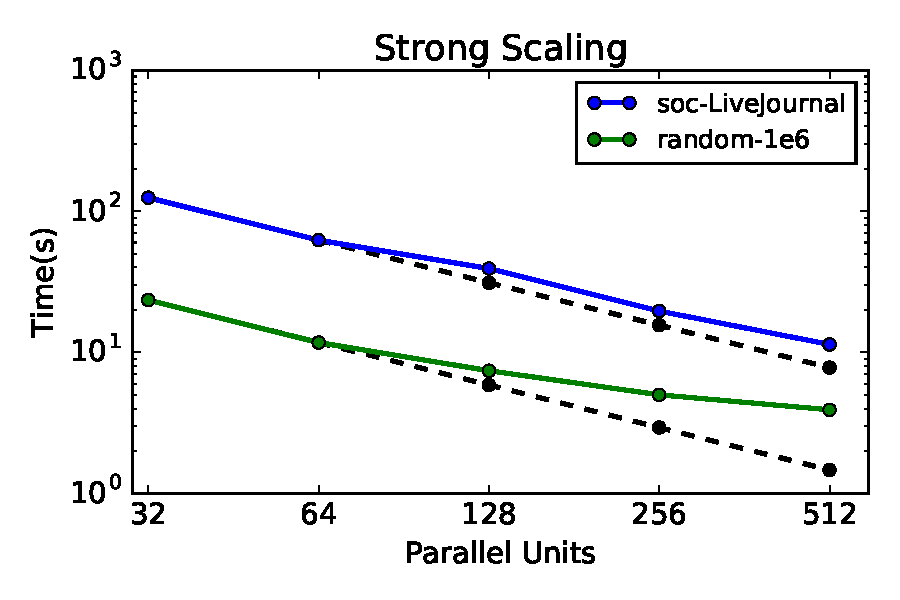
\includegraphics[width=0.45\textwidth]{img/strong-scaling-kpath.pdf}
%     \caption{\label{fig:scale-kpath} k-Path}
%   \end{subfigure}\\
  
%   \begin{subfigure}[b]{\textwidth}
%     \centering
%     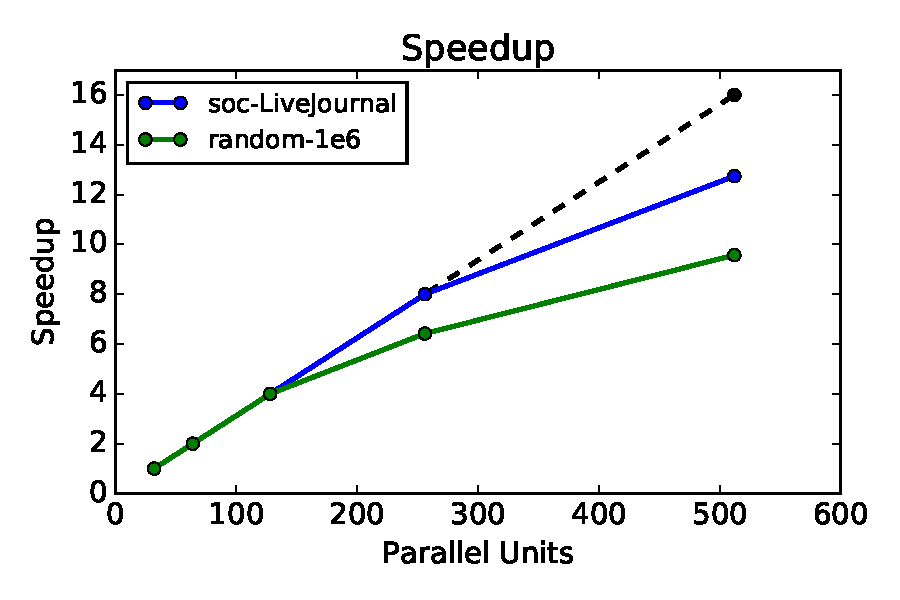
\includegraphics[width=0.45\textwidth]{img/speedup-multilinear.pdf}
%     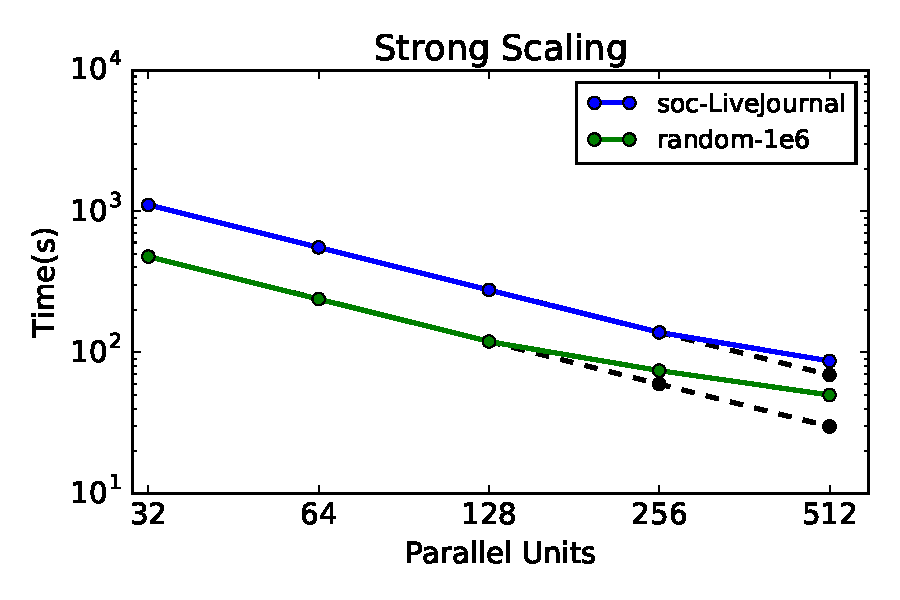
\includegraphics[width=0.45\textwidth]{img/strong-scaling-multilinear.pdf}
%     \caption{\label{fig:scale-multilinear} Multilinear Scan}
%   \end{subfigure}%
%   \caption{Speedup and strong scaling of our MPI algorithms for $k$-Path (\ref{fig:scale-kpath}) and Multilinear Scan (\ref{fig:scale-multilinear}).}
%  \label{fig:scaling}
% \end{figure*}

% \subsection{Comparision with Giraph}
% \label{sec:compare-giraph}
% %Performance for varying k=1 to k=16 in increments of 2
% %This can include both random-er and snap graphs
% We now compare our \parmaxwt{} with an implementation of Algorithm \ref{alg:multilinear-detect} in Giraph, which is a ``think like a vertex" computation framework. In Figure \ref{fig:giraph-comparison}, we show the running time of \parmaxwt{} and the Giraph implementation as a function of $k$. Giraph uses all the available parallel units for each of the $2^k$ circuit evaluation. Therefore, for a fair comparison, we report the time per iteration of both implementations---even though \parmaxwt{} runs multiple evaluations in parallel. Our MPI algorithm shows much better scalability with $k$, giving as much as 5x speed up  over Giraph in the LiveJournal network. We also implemented a version using Spark's GraphX library, but the communication cost associated with the dataflow model in Spark was prohibitively expensive for this algorithm. Giraph, on the other hand, follows a peer-to-peer communication model, similar to MPI, making it a better choice than GraphX.

% \begin{figure}[!htpb]
% 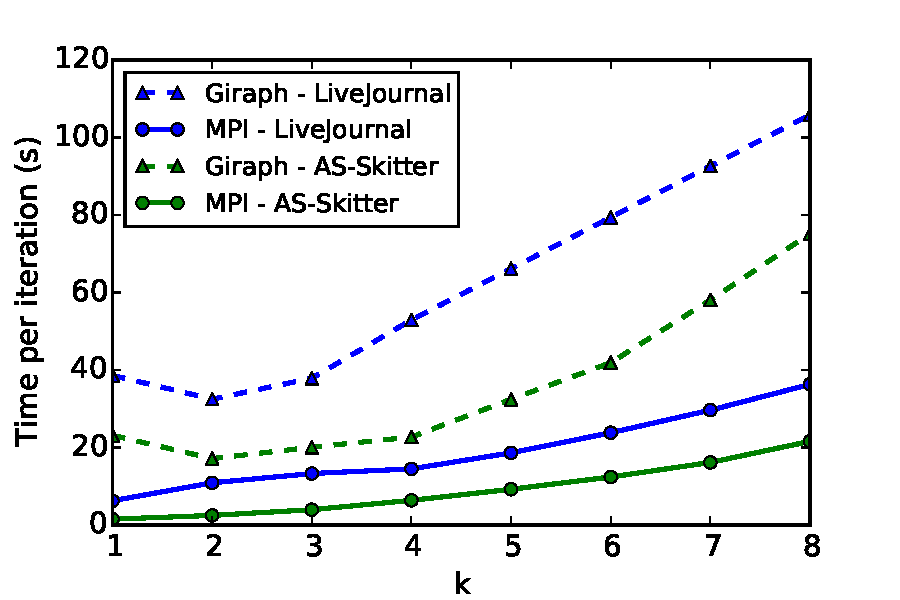
\includegraphics[width=0.4\textwidth]{img/giraph-comparison.pdf}
% \caption{Running time of \parmaxwt{} as a function of $k$ compared to a Giraph implementation.}
% \label{fig:giraph-comparison}
% \end{figure}



% \begin{figure}[!htpb]
% %\frame{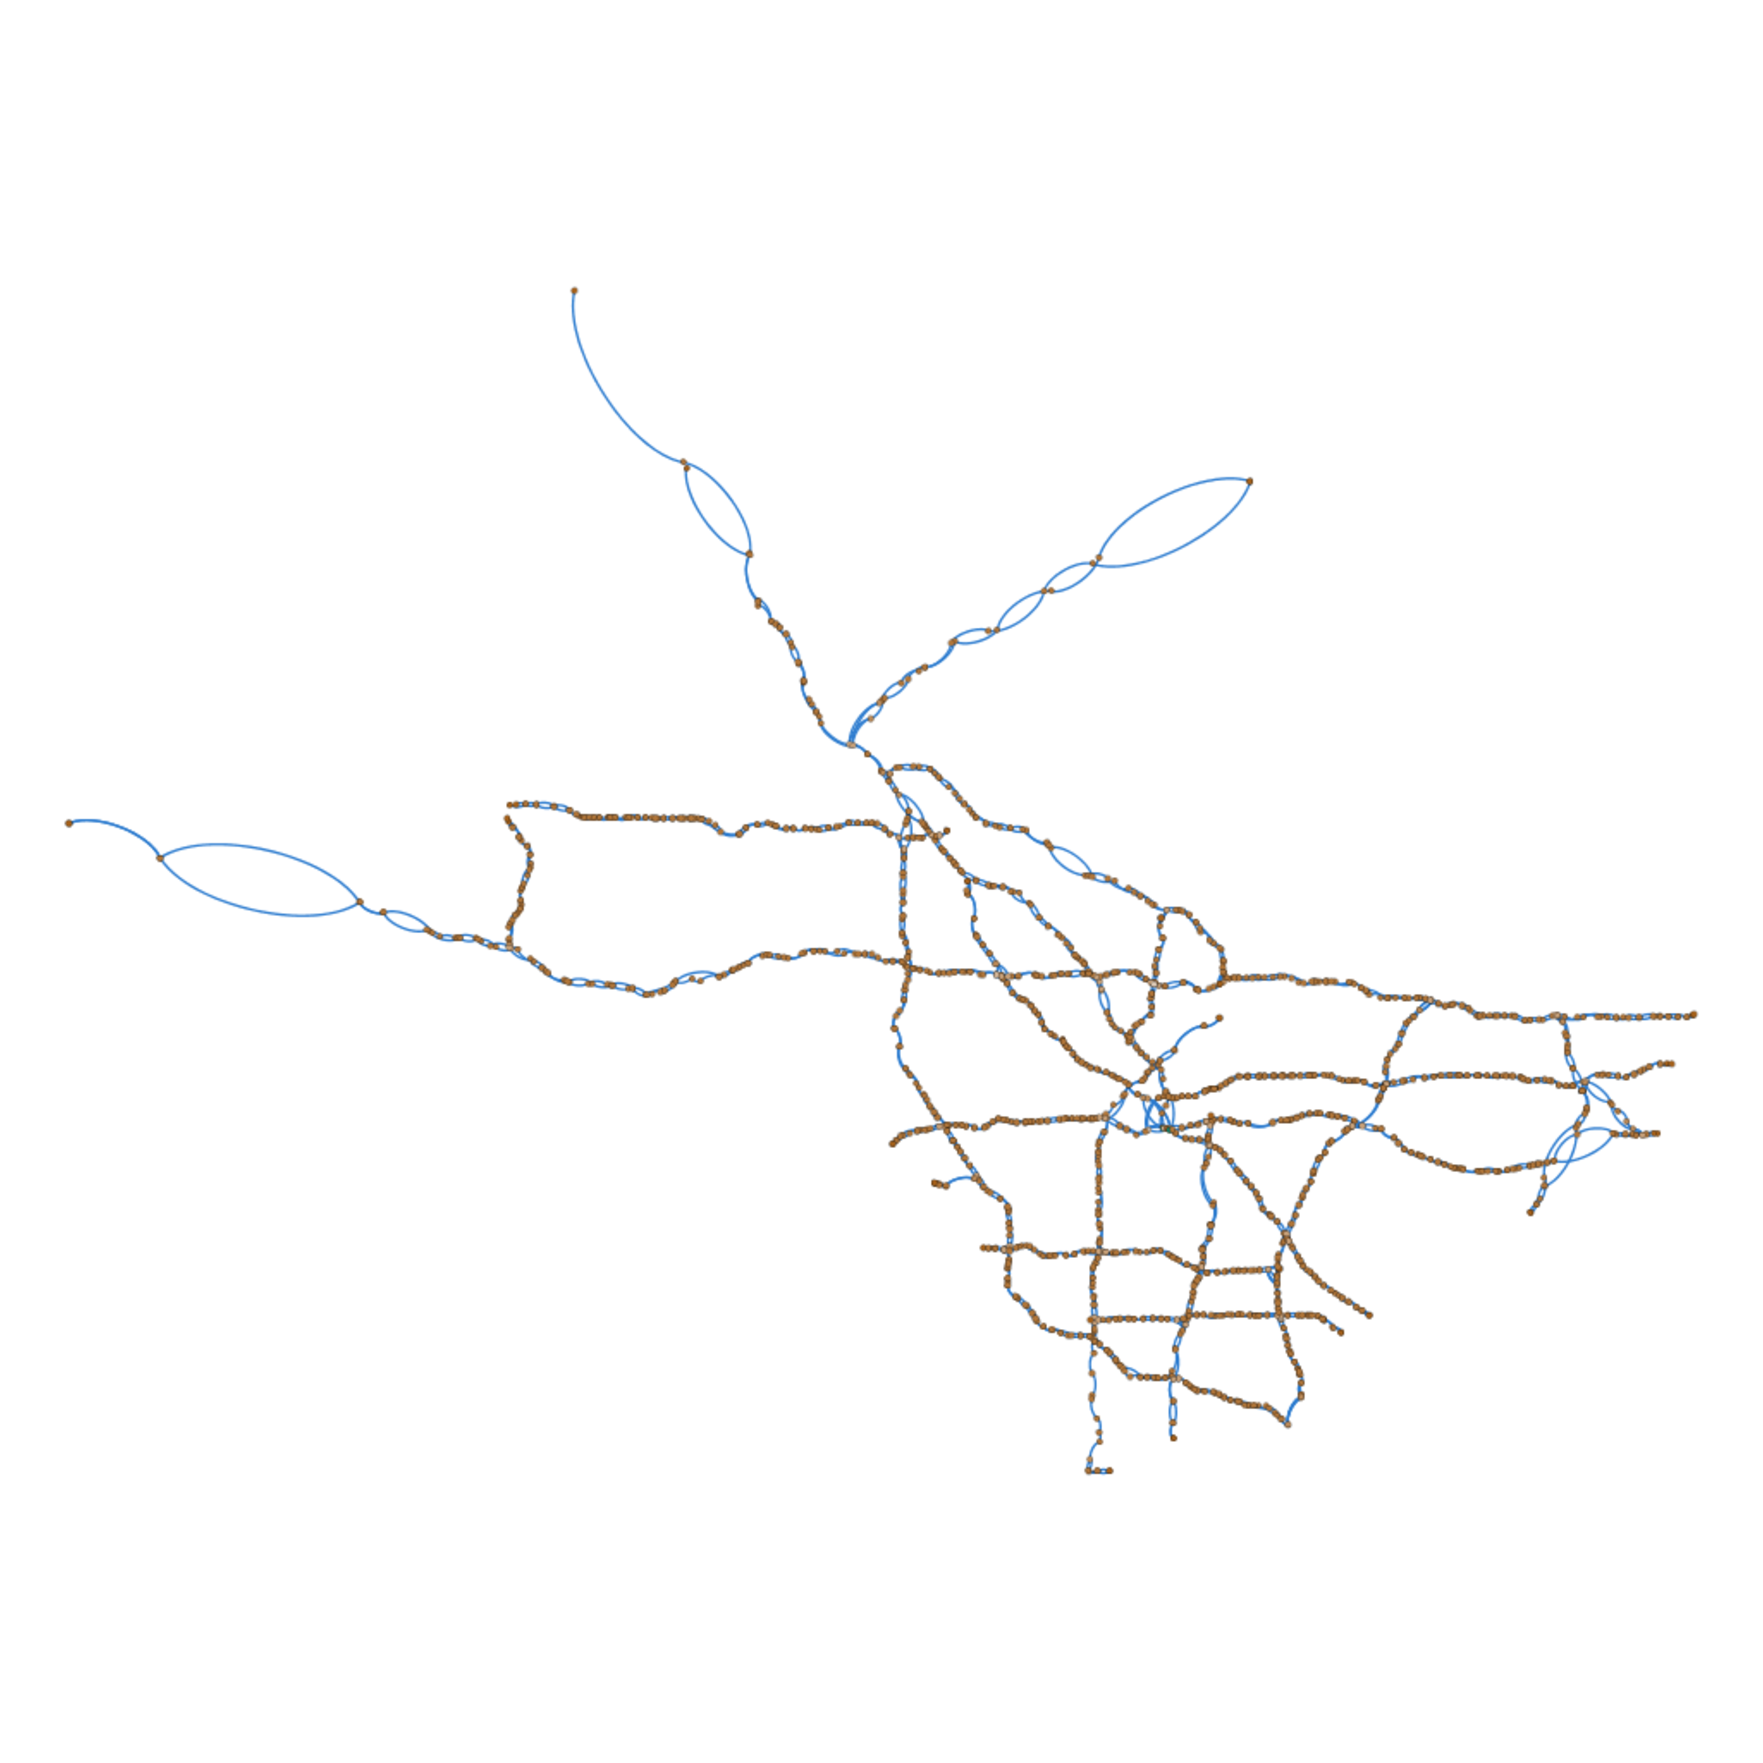
\includegraphics[width=0.48\textwidth,trim={0 4cm 0 4cm},clip]{img/traffic-network.pdf}}
% 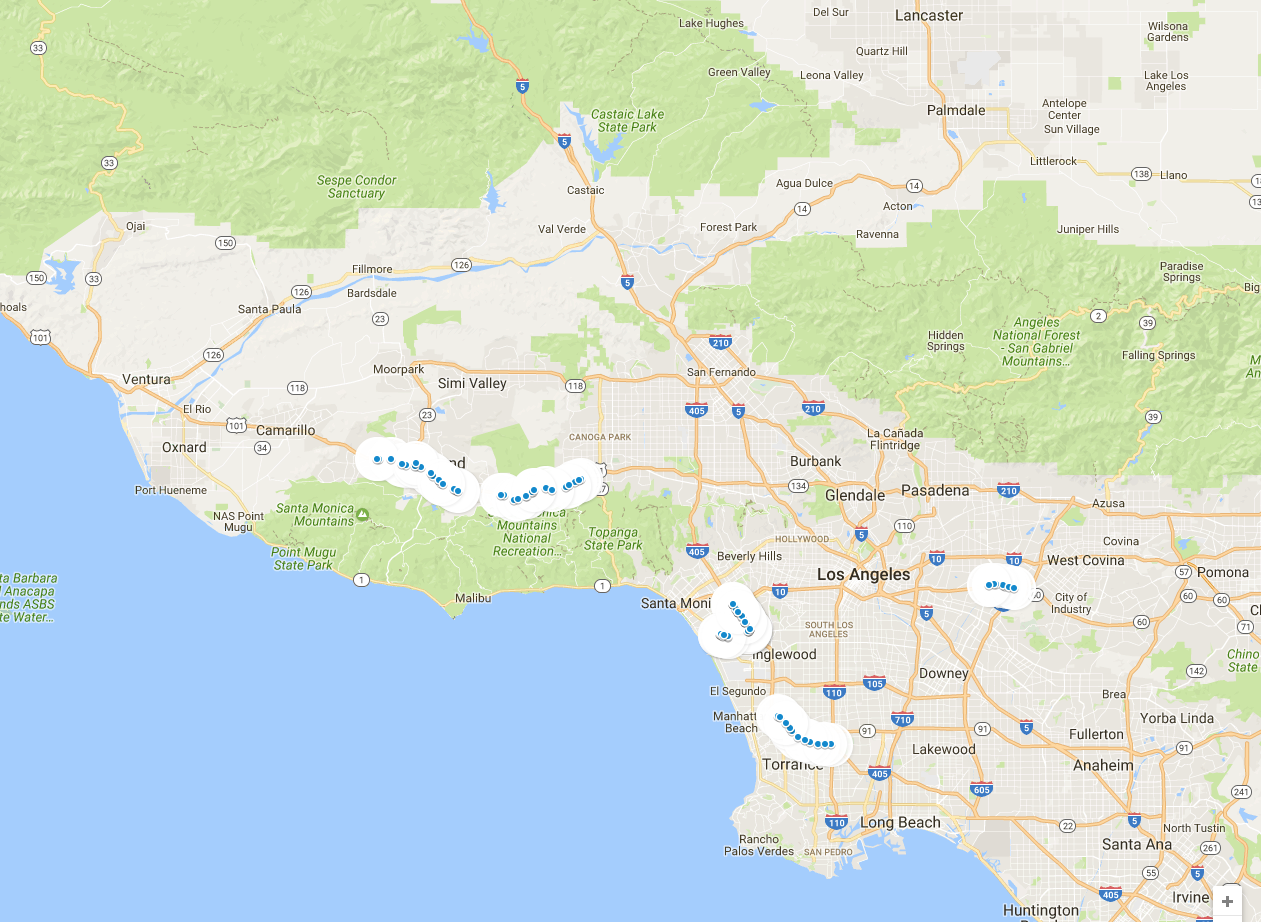
\includegraphics[width=0.48\textwidth]{img/traffic-example.png}
% \caption{Discovering highway segments with unexpected congesion in the Los Angeles road network.}
% \label{fig:traffic}
% \end{figure}



% !TEX root = ./multilinear.tex
\section{Related Work}
\label{sec:related}
There is a vast literature on a variety of subgraph analysis problems, arising
out of a number of applications, such as bioinformatics, security,
social network analysis, epidemiology and finance (see  \cite{akoglu2014graph} for a survey).
We discuss two main directions here: 
subgraph isomorphism and clique
enumeration---for which parallel algorithms exist---and anomaly detection---for which
there has been limited work on parallel algorithms.

% Given a graph $G=(V, E)$ with $n=|V|$, $m=|E|$, and a subgraph $H=(V_H, E_H)$, with $k=|V_H|$,
% the basic subgraph isomorphism problem involves finding a mapping $f:V_H\rightarrow V$
% such that $(i, j)\in E_H$ if and only if $(f(i), f(j))\in E$. This is
% a very computationally challenging problem. 
The basic frequent subgraph detection
problem involves finding subgraphs having  frequency higher than a threshold.
Parallel approaches for this problem involve a ``bottom-up'' candidate generation approach,
combined with careful pruning, which builds embeddings of larger subgraphs using all possible
embeddings of smaller subgraphs\cite{hamid2016scalemine, elsidy:vldb14}. While these results
allow scaling to very large networks with millions of nodes, they give no guarantees on
the performance. Our work is more closely related to the use of the color coding technique
for finding tree-like subgraphs \cite{alon2008biomolecular, huffner2008algorithm}, which
guarantees a fully polynomial time approximation to the number of embeddings with
running time and space of $O(2^ke^km\log{n})$ and $O(2^km)$, respectively.
This has been parallelized using MapReduce \cite{zhao2012sahad} and 
OpenMP \cite{slota:icpp13, slota:ipdps14}, enabling subgraph counting in graphs with
tens of millions of nodes with rigorous guarantees. Slota et al. \cite{slota:icpp13, slota:ipdps14}
use threading and techniques for reducing the memory footprint of the color coding
dynamic programming tables in order to scale. 
% Our approach uses algebraic methods
% for which the memory scales as $O(k)$ instead of $O(2^k)$, and the worst case
% running time scales as $O(2^k)$ instead of $O(2^ke^k)$, which gives the improved performance.
Another area where parallel algorithms have been developed is for dense subgraph enumeration.
% This is a very challenging problem, since finding the largest clique is NP-hard to
% approximate even within an $O(n^{1-\epsilon})$ factor for any $\epsilon>0$.
There are several implementations for finding maximal cliques in parallel by
careful partitioning, pruning and backtracking heuristics
\cite{schmidt2009scalable, zhao2016parallel, aparicio:ispa14, cheng:kdd12, du:mcd09}.
Our results do not extend to the clique enumeration problem.

Finally, there are only two prior works on parallel graph scan statistics \cite{cadena:bigdata17, zhao2016parallel}. However, these do not scale to very large instances.

% Finally, anomaly detection is a broad topic, and there has been some work
% on parallel algorithms, e.g., \cite{shanbhag:icccn08}. Our work is most related to
% the approach known as graph scan statistics, which involves finding connected subgraphs
% that optimize specific functions that model underlying processes about the data.
% While there exist a number of heuristics, the work of \cite{cadena:sdm17} gives the
% first rigorous methods for optimizing most scan statistics using the color coding technique.
% However, all these methods are sequential.

% !TEX root = ./multilinear.tex
\section{Conclusions}
\label{sec:conc}
State of the art parallel algorithms for various subgraph detection problems are based on the color coding technique, which yields algorithms with running time and space complexity proportional exponential on a solution size $k$. Here, we have presented algorithms based on a more recent technique from the parameterized complexity literature, multilinear detection. This methodology gives us improved bounds on memory and time over color coding. We propose an MPI algorithm for multilinear detection for general polynomials, and we show applications to two important problems, $k$-path and anomaly detection via scan statistics. We also show that finding a partitioning with minimum cost for the problem discussed here is NP-Hard, and we leave the development of partitioning heuristics as a topic of future work.

\bibliographystyle{IEEEtran}
\bibliography{refs}
%\newpage
%\input{appendix.tex}

% that's all folks
\end{document}